\documentclass{article} % For LaTeX2e
\usepackage{iclr2026_conference,times}

%--------------------------------------------------
% Standard packages
%--------------------------------------------------
\usepackage{amsmath,amssymb,amsthm,mathtools}
\usepackage{tikz}
\usetikzlibrary{fadings,patterns,shadows.blur,shapes,shapes.geometric}
\usepackage{array,booktabs,multirow,tabularx}
\usepackage{yhmath,mathdots,extarrows}
\usepackage{siunitx,gensymb}
\usepackage{physics,cancel,color,xcolor,xspace}
\usepackage{mdframed,thmtools}
\usepackage{pifont}
\usepackage[normalem]{ulem} % strikeout text
\usepackage{bbold}          % for \mathbb{1}
\usepackage{enumitem}
\usepackage{wrapfig}
\usepackage{algorithm}      % floating algorithm environment
\usepackage{algpseudocode}  % pseudocode macros (from algorithmicx package)

%--------------------------------------------------
% Hyperref setup
%--------------------------------------------------
\usepackage{hyperref}
\hypersetup{
    colorlinks=true,
    linkcolor=blue,
    citecolor=teal,
    urlcolor=magenta,
    pdfauthor={Your Name},
    pdftitle={Paper Title},
    pdfborder={0 0 0}
}
\usepackage{url}
\usepackage[sort&compress,capitalize,nameinlink]{cleveref}		% for cleveref formatting

%--------------------------------------------------
% Colors
%--------------------------------------------------
\definecolor{darkgreen}{RGB}{110,192,19}
\definecolor{shadecolor}{gray}{0.9}

%--------------------------------------------------
% Theorem styles
%--------------------------------------------------
\newtheoremstyle{informal}
  {3pt}{3pt}{\itshape}{}{\bfseries}{.}{ }
    {Main Result (Informal Theorem)}
%  {Main Result (Informal Theorem)~\thmnumber{#2}}

\theoremstyle{informal}
\newtheorem*{maininformal}{}
%\newtheorem{maininformal}{}

\newtheoremstyle{remark}
  {3pt}{3pt}{\itshape}{}{\bfseries}{.}{ }
%    {Main Result (Informal Theorem)}
  {Remark~\thmnumber{#2}}
\theoremstyle{remark}
\newtheorem{draftremark}{}

\declaretheoremstyle[
  headfont=\normalfont\bfseries,
  notefont=\mdseries, notebraces={(}{)},
  bodyfont=\normalfont,
  postheadspace=0.5em,
  spaceabove=1pt,
  mdframed={
    skipabove=8pt, skipbelow=8pt,
    hidealllines=true,
    backgroundcolor={shadecolor},
    innerleftmargin=4pt,
    innerrightmargin=4pt}
]{shaded}

\declaretheorem[style=shaded,within=section]{definition}
\declaretheorem[style=shaded,sibling=definition]{theorem}
\declaretheorem[style=shaded,sibling=definition]{proposition}
\declaretheorem[style=shaded,sibling=definition]{assumption}
\declaretheorem[style=shaded,sibling=definition]{corollary}
\declaretheorem[style=shaded,sibling=definition]{lemma}
\declaretheorem[style=shaded,sibling=definition]{example}


%--------------------------------------------------
% Editing / debugging helpers
%--------------------------------------------------
\newcommand{\debug}[1]{#1}
\newcommand{\kostas}[1]{\textcolor{blue}{[Kostas: #1]}}

%--------------------------------------------------
% Handy wrappers for operators/macros
%--------------------------------------------------
\newcommand{\textbrac}[1]{\textup[#1\textup]}
\newcommand{\textpar}[1]{\textup(#1\textup)}
\newcommand{\newmacro}[2]{\newcommand{#1}{\debug{#2}}}
\newcommand{\newop}[2]{\DeclareMathOperator{#1}{\debug{#2}}}

%--------------------------------------------------
% Custom macros (RR, noise, prob, expectations, etc.)
%--------------------------------------------------
\newcommand{\RRresh}{\texttt{RR}\textsubscript{1}} % Random Reshuffling
\newcommand{\RRrom}{\texttt{RR}\textsubscript{2}}  % Richardson–Romberg
\newcommand{\gammaub}{\min\left\{\frac{1}{3nL_{max}}, \frac{\sqrt{1+6 \mu^2 L_{max}^2} -1}{12nL_{max}^2}\right\}}
\newcommand{\gammaubmoments}{\min\left\{\frac{\mu}{3nL_{max}^2}, \frac{\sqrt{1+6 \mu^2 L_{max}^2} -1}{12nL_{max}^2}, \frac{\mu^{3/5}}{8nL_{max}^{3/5}}\right\}}
\newcommand{\gammaubbothrr}{\min\left\{\frac{\mu}{3nL_{max}^2}, \frac{\sqrt{1+6 \mu^2 L_{max}^2} -1}{12nL_{max}^2}, \frac{\mu^{3/5}}{8nL_{max}^{3/5}}\right\}}
\newcommand{\as}{\debug{\textpar{a.s.}}\xspace}

%% Math commands 
\newcommand{\R}{\mathbb{R}}
\newcommand{\Var}{\operatorname{\textrm{Var}}}
\newcommand{\goto}{\rightarrow}
\newcommand{\sgn}{\mathop\mathrm{sgn}}
\newcommand{\N}{\mathcal{N}}
\newcommand{\A}{\mathcal{A}}
\newcommand{\F}{\mathcal{F}}
\renewcommand{\P}{\operatorname{\mathbb{P}}}
\newcommand{\E}{\operatorname{\mathbb{E}}}
\newcommand{\e}{\mathrm{e}}
\renewcommand\d{\operatorname{\mathrm{d}}}
\newcommand{\deq}{\overset{\mathrm{d}}{=}}
\newcommand{\EE}{\operatorname{\mathbb{E}}}
% \newcommand{\eps}{{\epsilon}}
\newcommand{\cO}{\operatorname{\mathcal{O}}}
\newcommand{\RR}{\operatorname{\mathbb{R}}}

\newcommand{\nullspace}{{\mathcal N}}
\newcommand{\range}{{\mathcal R}}
\newcommand{\Rank}{\mathop{\bf Rank}}
% \newcommand{\diag}{\mathop{\bf diag}}
% \newcommand{\card}{\mathop{\bf card}}
% \newcommand{\rank}{\mathop{\bf rank}}
% \newcommand{\conv}{\mathop{\bf conv}}
% \newcommand{\prox}{\mathbf{prox}}
% \newcommand{\proj}{\mathbf{proj}}

\newop{\ex}{\mathbb{E}}     % expectation
\newop{\prob}{\mathbb{P}}   % probability
\newop{\simplex}{\hull}

\newmacro{\noise}{U}
\newmacro{\filter}{\mathcal{F}}
\newmacro{\sgda}{\text{SGDA}}
\newmacro{\seg}{\text{SEG}}
\newcommand{\Expep}[1]{\ex\left[#1 \Big| \filter_k\right]}
\newcommand{\Expepgamma}[1]{\ex_{\pi_{\gamma}}\left[#1 \right]}
\newcommand{\ie}{i.e.,\xspace}

%--------------------------------------------------
% Geometry / sets / points
%--------------------------------------------------
\newmacro{\point}{x}
\newmacro{\pointalt}{\alt\point}
\newmacro{\pointaltalt}{\altalt\point}
\newmacro{\points}{\mathcal{X}}
\newmacro{\intpoints}{\relint\points}
\newmacro{\base}{p}
\newmacro{\basealt}{q}
\newmacro{\basealtalt}{u}
\newmacro{\open}{\mathcal{U}}
\newmacro{\closed}{\mathcal{C}}
\newmacro{\cpt}{\mathcal{K}}
\newmacro{\nhd}{\mathcal{U}}
\newmacro{\gmat}{g}
\newmacro{\gdist}{\dist_{\gmat}}
\newmacro{\mfld}{M}
\newmacro{\form}{\omega}
\newmacro{\tvec}{z}
\newmacro{\uvec}{u}
\newmacro{\basin}{\mathbb{B}}
\newmacro{\ball}{\basin}
\newmacro{\sphere}{\mathbb{S}}


%----------------------------------------------------------------------
%% Dynamical systems
%----------------------------------------------------------------------
\newmacro{\tstart}{0}		% for time start
\renewcommand{\time}{\debug{t}}		% for continuous time
\newmacro{\timealt}{s}		% for dummy continuous time
\newmacro{\horizon}{T}		% for horizon

\newmacro{\traj}{x}		% for trajectory
\newmacro{\trajalt}{y}		% for variant trajectory
\newmacro{\trajaltalt}{z}		% for second variant

\newmacro{\flowmap}{\Theta}		% for (semi)flow map
\DeclarePairedDelimiterXPP{\flowof}[2]{\flowmap_{#1}}{(}{)}{}{#2}		% for flow



%----------------------------------------------------------------------
%% Optimization (basics)
%----------------------------------------------------------------------
\newop{\Opt}{Opt}		% for value of problem
\newop{\Sol}{Sol}		% for solution of problem
\newop{\gap}{Gap}	
\newop{\dualitygap}{Duality-Gap}		% for gap function
% for gap function
\newop{\orcl}{Or}		% for oracle

\newmacro{\tfun}{f}		% for test function
\newmacro{\obj}{f}		% for objective function
\newmacro{\objalt}{g}		% for variant objective (smooth etc.)
\newmacro{\sobj}{F}		% for stochastic objective

\newmacro{\gvec}{g}		% for gradient vector
\newmacro{\oper}{A}		% for operator
\newmacro{\vecfield}{v}		% for vector field (selection etc.)
%\newmacro{\payfield}{v}		% for payoff field (selection etc.)

\newcommand{\sol}[1][\point]{#1^{\ast}}		% for solution point (x by default)
\newcommand{\sols}{\sol[\points]}		% for set of solutions
\newmacro{\solvec}{\vecfield(\sol)}		% for vector at a solution
\newmacro{\solpay}{\eq[\payv]}		% for vector at a solution

\newcommand{\test}[1][\point]{\hat#1}		% for test point (x by default)

\newmacro{\signal}{V}		% for signal
\newmacro{\step}{\gamma}		% for step-size
\newmacro{\learn}{\eta}		% for learning rate

\newmacro{\vbound}{G}		% for vector bound
\newmacro{\lips}{\ell}		% for Lipschitz modulus
\newmacro{\strong}{\mu}		% for strong convexity modulus
\newmacro{\smooth}{\beta}		% for strong smoothness modulus


%----------------------------------------------------------------------
%% Optimization (convex analysis)
%----------------------------------------------------------------------
\newop{\tspace}{T}		% for tangent space
\newop{\tcone}{TC}		% for tangent cone
\newop{\dcone}{\tcone^{\ast}}		% for dual cone
\newop{\ncone}{NC}		% for normal cone
\newop{\pcone}{PC}		% for polar cone
\newop{\hull}{\Delta}		% for hull

\newmacro{\cvx}{\mathcal{C}}		% for generic convex set
\newmacro{\subd}{\partial}		% for subdifferential
\newcommand{\subsel}{\nabla}		% for subdifferential


%----------------------------------------------------------------------
%% Optimization (min-max)
%----------------------------------------------------------------------
\newmacro{\minmax}{\mathcal{L}}		% for minmax objective

\newmacro{\minvar}{{\point_{1}}}		% for minimization variable
\newmacro{\minvaralt}{\alt\minvar}		% for variant minvar
\newmacro{\minvars}{\points_{1}}		% for set of minvars
\newmacro{\minsol}{\sol[\minvar]}		% for min solution

\newmacro{\maxvar}{\point_{2}}		% for maximization variable
\newmacro{\maxvaaltr}{\alt\maxvar}		% for variant maxvar
\newmacro{\maxvars}{\points_{2}}		% for set of maxvars
\newmacro{\maxsol}{\sol[\maxvar]}		% for max solution


%----------------------------------------------------------------------
%% Optimization (mirror descent)
%----------------------------------------------------------------------
\newop{\Eucl}{\Pi}		% for Euclidean projection
\newop{\logit}{\Lambda}		% for logit map
\newop{\dkl}{KL}		% for Kullback Leibler

\newmacro{\hreg}{h}		% for regularizer
\newmacro{\hconj}{\hreg^{\ast}}		% for regularizer
\newmacro{\breg}{D}		% for Bregman divergence
\newmacro{\mprox}{P}		% for Bregman prox-mapping
\newmacro{\mirror}{Q}		% for mirror map
\newmacro{\fench}{F}		% for Fenchel coupling
\newmacro{\depth}{H}		% for regularizer depth
\newmacro{\hstr}{K}		% for strong convexity constant
\newmacro{\hker}{\theta}		% for regularizer kernel

\newmacro{\proxdom}{\points_{\hreg}}		% for prox-domain
\newmacro{\proxdomi}{\points_{\hreg_{\play}}}		% for prox-domain of player i
\newmacro{\zone}{\mathbb{D}}		% for Bregman zone

\DeclarePairedDelimiterXPP{\proxof}[2]{\mprox_{#1}}{(}{)}{}{#2}		% for Bregman prox step

\newcommand{\lazy}[1]{#1^{\textup{lazy}}}		% for lazy iterate
\newcommand{\eager}[1]{#1^{\textup{eager}}}		% for eager iterate



%--------------------------------------------------
% Algorithms / states
%--------------------------------------------------
\newmacro{\state}{x}
\newmacro{\statealt}{y}
\newmacro{\statealtalt}{z}
\newmacro{\solb}{\mathrm{R}}
\newmacro{\growth}{L}
\newmacro{\wqsmscale}{\mu}
\newmacro{\wqsmshift}{\lambda}
\newcommand{\steps}[1]{\gamma^{\text{\tiny #1}}}
\newcommand{\stepsalt}[1]{\alpha^{\text{\tiny #1}}}
\newmacro{\stepalt}{\alpha}
\newcommand{\deltaminor}[1]{\delta^{\braces{\text{\tiny #1}}}}
\newcommand{\cnstminor}[1]{c_1^{\braces{\text{\tiny #1}}}}
\newcommand{\cnstminoralt}[1]{c_2^{\braces{\text{\tiny #1}}}}
\newcommand{\cnstsminor}[1]{(c_1,c_2)^{\braces{\text{\tiny {#1}}}}}
\newmacro{\rvar}{g}
\newmacro{\kyrt}{\delta_{\text{\tiny{KYRT}}}}
\newmacro{\energy}{\mathcal{E}}
\newcommand{\meas}[1]{\nu^{\text{\tiny #1}}}
\newmacro{\irr}{\psi}
\newcommand{\distr}[2]{\pi_{#2}^{\braces{\text{\tiny #1}}}}
\newmacro{\set}{C}
\newmacro{\tf}{\phi}
\newcommand{\tconst}[1]{\rho^{\braces{\text{\tiny #1}}}}
\newcommand{\tconstalt}[1]{\kappa^{\braces{\text{\tiny #1}}}}
\newcommand{\law}{\text{law}}
\newmacro{\normal}{\mathcal{N}}
\newmacro{\thres}{\theta}
\newmacro{\borel}{\mathcal{B}}
\newcommand{\snorm}{\norm{\state_\time-\state^*}}
\newcommand{\ssnorm}{\norm{\state-\state^*}}

%--------------------------------------------------
% Delimiters
%--------------------------------------------------
\DeclarePairedDelimiter{\ourbraces}{\{}{\}}
\DeclarePairedDelimiter{\bracks}{[}{]}
\DeclarePairedDelimiter{\parens}{(}{)}
\DeclarePairedDelimiter{\clip}{[}{]}
\DeclarePairedDelimiter{\negpart}{[}{]_{-}}
\DeclarePairedDelimiter{\pospart}{[}{]_{+}}
\DeclarePairedDelimiter{\setof}{\lbrace}{\rbrace}
\DeclarePairedDelimiterX{\setdef}[2]{\lbrace}{\rbrace}{#1:#2}
\DeclarePairedDelimiterX{\inner}[2]{\langle}{\rangle}{#1,#2}
\DeclarePairedDelimiterXPP{\exclude}[1]{\mathopen{}\setminus}{\lbrace}{\rbrace}{}{#1}

\providecommand\given{} % empty for conditional bar
\DeclarePairedDelimiterXPP{\exof}[1]{\ex}{\Big[}{\Big]}{}{%
  \renewcommand\given{\nonscript\,\delimsize\vert\nonscript\,\mathopen{}} #1}
\DeclarePairedDelimiterXPP{\probof}[1]{\prob}{(}{)}{}{%
  \renewcommand\given{\nonscript\:\delimsize\vert\nonscript\:\mathopen{}} #1}
\DeclarePairedDelimiterXPP{\oneof}[1]{\one}{\lbrace}{\rbrace}{}{%
  \renewcommand\given{\nonscript\,\delimsize\vert\nonscript\,\mathopen{}} #1}

\newcommand{\Expe}[1]{\exof{#1}}

%--------------------------------------------------
% Operators
%--------------------------------------------------
\DeclareMathOperator*{\intersect}{\bigcap}
\DeclareMathOperator*{\union}{\bigcup}
\DeclareMathOperator{\aff}{aff}
\DeclareMathOperator{\lspan}{span}
\DeclareMathOperator{\bd}{bd}
\DeclareMathOperator{\littleoh}{o}
\DeclareMathOperator{\bigoh}{\mathcal{O}}
\DeclareMathOperator{\card}{card}
\DeclareMathOperator{\cl}{cl}
\DeclareMathOperator{\conv}{conv}
\DeclareMathOperator{\crit}{crit}
\DeclareMathOperator{\diam}{diam}
\DeclareMathOperator{\dist}{dist}
\DeclareMathOperator{\eig}{eig}
\DeclareMathOperator{\ess}{ess}
\DeclareMathOperator{\Hess}{Hess}
\DeclareMathOperator{\ind}{ind}
\DeclareMathOperator{\im}{im}
\DeclareMathOperator{\intr}{int}
\DeclareMathOperator{\Jac}{Jac}
\DeclareMathOperator{\one}{\mathbb{1}} % indicator
\DeclareMathOperator{\proj}{pr}
\DeclareMathOperator{\prox}{prox}
\DeclareMathOperator{\relint}{ri}
\DeclareMathOperator{\supp}{supp}
\DeclareMathOperator{\Sym}{Sym}
\DeclareMathOperator{\unif}{unif}
\DeclareMathOperator{\vol}{vol}

%%%%%%%%%
%%%%%%%%%\documentclass{article} % For LaTeX2e
%%%%%%%%%\usepackage{iclr2026_conference,times}
%%%%%%%%%
%%%%%%%%%% Optional math commands from https://github.com/goodfeli/dlbook_notation.
%%%%%%%%%\input{math_commands.tex}
%%%%%%%%%
%%%%%%%%%\usepackage{hyperref}
%%%%%%%%%% --- Hyperref setup ---
%%%%%%%%%\hypersetup{
%%%%%%%%%    colorlinks=true,
%%%%%%%%%    linkcolor=blue,
%%%%%%%%%    citecolor=teal,
%%%%%%%%%    urlcolor=magenta,
%%%%%%%%%    pdfauthor={Your Name},
%%%%%%%%%    pdftitle={Paper Title},
%%%%%%%%%    pdfborder={0 0 0}
%%%%%%%%%}
%%%%%%%%%\usepackage{url}
%%%%%%%%%\usepackage{cancel}
%%%%%%%%%\usepackage{physics}
%%%%%%%%%\usepackage{amsmath}
%%%%%%%%%\usepackage{tikz}
%%%%%%%%%\usepackage{mathdots}
%%%%%%%%%\usepackage{yhmath}
%%%%%%%%%\usepackage{cancel}
%%%%%%%%%\usepackage{color}
%%%%%%%%%\usepackage{siunitx}
%%%%%%%%%\usepackage{array}
%%%%%%%%%\usepackage{multirow}
%%%%%%%%%\usepackage{amssymb}
%%%%%%%%%\usepackage{gensymb}
%%%%%%%%%\usepackage{tabularx}
%%%%%%%%%\usepackage{extarrows}
%%%%%%%%%\usepackage{booktabs}
%%%%%%%%%\usetikzlibrary{fadings}
%%%%%%%%%\usetikzlibrary{patterns}
%%%%%%%%%\usetikzlibrary{shadows.blur}
%%%%%%%%%\usetikzlibrary{shapes}
%%%%%%%%%\usetikzlibrary{shapes.geometric}
%%%%%%%%%
%%%%%%%%%\usepackage{xcolor}
%%%%%%%%%
%%%%%%%%%% Define the dark green color
%%%%%%%%%\definecolor{darkgreen}{RGB}{110,192,19}
%%%%%%%%%
%%%%%%%%%\usepackage{amsthm}
%%%%%%%%%
%%%%%%%%%\newtheoremstyle{informal}   % name
%%%%%%%%%  {3pt}                      % Space above
%%%%%%%%%  {3pt}                      % Space below
%%%%%%%%%  {\itshape}                 % Body font
%%%%%%%%%  {}                         % Indent amount
%%%%%%%%%  {\bfseries}                % Theorem head font
%%%%%%%%%  {.}                        % Punctuation after theorem head
%%%%%%%%%  { }                        % Space after theorem head
%%%%%%%%%  {Main Result (Informal Theorem)~\thmnumber{#2}} % Theorem head spec
%%%%%%%%%
%%%%%%%%%\theoremstyle{informal}
%%%%%%%%%\newtheorem{maininformal}{}
%%%%%%%%%%%%%%%%%%% SHADED COLORS %%%%%%%%%%%%%%%%
%%%%%%%%%% \let\proof\undefined
%%%%%%%%%\usepackage{mdframed}
%%%%%%%%%\usepackage{thmtools}
%%%%%%%%%
%%%%%%%%%\definecolor{shadecolor}{gray}{0.9}
%%%%%%%%%\declaretheoremstyle[
%%%%%%%%%headfont=\normalfont\bfseries,
%%%%%%%%%notefont=\mdseries, notebraces={(}{)},
%%%%%%%%%bodyfont=\normalfont,
%%%%%%%%%postheadspace=0.5em,
%%%%%%%%%spaceabove=1pt,
%%%%%%%%%mdframed={
%%%%%%%%%  skipabove=8pt,
%%%%%%%%%  skipbelow=8pt,
%%%%%%%%%  hidealllines=true,
%%%%%%%%%  backgroundcolor={shadecolor},
%%%%%%%%%  innerleftmargin=4pt,
%%%%%%%%%  innerrightmargin=4pt}
%%%%%%%%%]{shaded}
%%%%%%%%%
%%%%%%%%%\declaretheorem[style=shaded,within=section]{definition}
%%%%%%%%%\declaretheorem[style=shaded,sibling=definition]{theorem}
%%%%%%%%%\declaretheorem[style=shaded,sibling=definition]{proposition}
%%%%%%%%%\declaretheorem[style=shaded,sibling=definition]{assumption}
%%%%%%%%%\declaretheorem[style=shaded,sibling=definition]{corollary}
%%%%%%%%%% \declaretheorem[style=shaded,sibling=definition]{conjecture}
%%%%%%%%%\declaretheorem[style=shaded,sibling=definition]{lemma}
%%%%%%%%%% \declaretheorem[style=shaded,sibling=definition]{remark}
%%%%%%%%%\declaretheorem[style=shaded,sibling=definition]{example}
%%%%%%%%%
%%%%%%%%%\usepackage{pifont}
%%%%%%%%%\usepackage[normalem]{ulem}		% for strikeout text
%%%%%%%%%\usepackage{xspace}
%%%%%%%%%
%%%%%%%%%%\usepackage[suppress]{color-edits}		% for editing macros / use [suppress] for final
%%%%%%%%%
%%%%%%%%%% \newcommand{\debug}[1]{{\color{RevColor}#1}}		% for macro coloring
%%%%%%%%%\newcommand{\debug}[1]{#1}		% for removing macro coloring
%%%%%%%%%\newcommand{\textbrac}[1]{\textup[#1\textup]}		% for upshape brackets
%%%%%%%%%\newcommand{\textpar}[1]{\textup(#1\textup)}		% for upshape parentheses
%%%%%%%%%\newcommand{\newmacro}[2]{\newcommand{#1}{\debug{#2}}}		% for shorthand definitions
%%%%%%%%%\newcommand{\newop}[2]{\DeclareMathOperator{#1}{\debug{#2}}}		% for shorthand definitions
%%%%%%%%%\newcommand{\RRresh}{\texttt{RR}\textsubscript{1}} % Random Reshuffling
%%%%%%%%%\newcommand{\RRrom}{\texttt{RR}\textsubscript{2}}  % Richardson–Romberg
%%%%%%%%%\newcommand{\gammaub}{\frac{1}{3nL_{max}}}
%%%%%%%%%\newcommand{\as}{\debug{\textpar{a.s.}}\xspace}		% for almost surely
%%%%%%%%%\newop{\ex}{\mathbb{E}}		% for expectations
%%%%%%%%%\newop{\prob}{\mathbb{P}}		% for probability
%%%%%%%%%\newop{\simplex}{\hull}
%%%%%%%%%\newmacro{\noise}{U}		% for noise
%%%%%%%%%\newmacro{\filter}{\mathcal{F}}	
%%%%%%%%%\newmacro{\sgda}{\text{SGDA}}
%%%%%%%%%\newmacro{\seg}{\text{SEG}}	% for filtration
%%%%%%%%%\newcommand{\Expep}[1]{\ex\left[#1 \Big| \filter_k\right]}
%%%%%%%%%\newcommand{\Expepgamma}[1]{\ex_{\pi_{\gamma}}\left[#1 \Big| \filter_k\right]}
%%%%%%%%%\newcommand{\ie}{i.e.,\xspace}		% for consistency
%%%%%%%%%
%%%%%%%%%
%%%%%%%%%%----------------------------------------------------------------------
%%%%%%%%%%% Points and sets
%%%%%%%%%%----------------------------------------------------------------------
%%%%%%%%%\newmacro{\point}{x}		% for generic point
%%%%%%%%%\newmacro{\pointalt}{\alt\point}		% for variant point
%%%%%%%%%\newmacro{\pointaltalt}{\altalt\point}		% for second variant
%%%%%%%%%\newmacro{\points}{\mathcal{X}}		% for set of points
%%%%%%%%%\newmacro{\intpoints}{\relint\points}		%for point set interior
%%%%%%%%%
%%%%%%%%%\newmacro{\base}{p}		% for reference point
%%%%%%%%%\newmacro{\basealt}{q}		% for variant reference point
%%%%%%%%%\newmacro{\basealtalt}{u}		% for second variant
%%%%%%%%%
%%%%%%%%%\newmacro{\open}{\mathcal{U}}		% for open sets
%%%%%%%%%\newmacro{\closed}{\mathcal{C}}		% for closed sets
%%%%%%%%%\newmacro{\cpt}{\mathcal{K}}		% for compact sets
%%%%%%%%%\newmacro{\nhd}{\mathcal{U}}		% for neighborhoods
%%%%%%%%%
%%%%%%%%%
%%%%%%%%%
%%%%%%%%%%----------------------------------------------------------------------
%%%%%%%%%%% Geometry
%%%%%%%%%%----------------------------------------------------------------------
%%%%%%%%%\newmacro{\gmat}{g}		% for metric tensor
%%%%%%%%%\newmacro{\gdist}{\dist_{\gmat}}
%%%%%%%%%\newmacro{\mfld}{M}		% for manifold
%%%%%%%%%\newmacro{\form}{\omega}		% for generic form
%%%%%%%%%
%%%%%%%%%\newmacro{\tvec}{z}		% for tangent vector
%%%%%%%%%\newmacro{\uvec}{u}		% for unit vector
%%%%%%%%%\newmacro{\basin}{\mathbb{B}}
%%%%%%%%%\newmacro{\ball}{\basin}		% for ball
%%%%%%%%%\newmacro{\sphere}{\mathbb{S}}		% for sphere
%%%%%%%%%
%%%%%%%%%
%%%%%%%%%
%%%%%%%%%%----------------------------------------------------------------------
%%%%%%%%%%% Algorithms (states and recursions)
%%%%%%%%%%----------------------------------------------------------------------
%%%%%%%%%\newmacro{\state}{x}		% for main iterate
%%%%%%%%%\newmacro{\statealt}{y}		% for variant state
%%%%%%%%%\newmacro{\statealtalt}{z}		% for second variant
%%%%%%%%%
%%%%%%%%%
%%%%%%%%%
%%%%%%%%%\newmacro{\solb}{\mathrm{R}} %for bound of the solution
%%%%%%%%%\newmacro{\growth}{L} %for the linear growth
%%%%%%%%%\newmacro{\wqsmscale}{\mu} %for the scaling parameter of wqsm
%%%%%%%%%\newmacro{\wqsmshift}{\lambda} %for the shifting parameter of wqsm
%%%%%%%%%\newcommand{\steps}[1]{\gamma^{\text{\tiny #1}}}
%%%%%%%%%\newcommand{\stepsalt}[1]{\alpha^{\text{\tiny #1}}}
%%%%%%%%%\newmacro{\stepalt}{\alpha}
%%%%%%%%%\newcommand{\deltaminor}[1]{\delta^{\braces{\text{\tiny #1}}}}
%%%%%%%%%\newcommand{\cnstminor}[1]{c_1^{\braces{\text{\tiny #1}}}} %constant for minorization
%%%%%%%%%\newcommand{\cnstminoralt}[1]{c_2^{\braces{\text{\tiny #1}}}} %constant for minorization
%%%%%%%%%\newcommand{\cnstsminor}[1]{(c_1,c_2)^{\braces{\text{\tiny {#1}}}}} %for pair of constants in minor
%%%%%%%%%\newmacro{\rvar}{g}
%%%%%%%%%\newmacro{\kyrt}{\delta_{\text{\tiny{ KYRT}}}}
%%%%%%%%%\newmacro{\energy}{\mathcal{E}}
%%%%%%%%%\newcommand{\meas}[1]{\nu^{\text{\tiny #1}}}
%%%%%%%%%\newmacro{\irr}{\psi}
%%%%%%%%%\newcommand{\distr}[2]{\pi_{#2}^{\braces{\text{\tiny #1}}}}
%%%%%%%%%\newmacro{\set}{C}
%%%%%%%%%\newmacro{\tf}{\phi}
%%%%%%%%%\newcommand{\tconst}[1]{\rho^{\braces{\text{\tiny #1}}}}
%%%%%%%%%\newcommand{\tconstalt}[1]{\kappa^{\braces{\text{\tiny #1}}}}
%%%%%%%%%\newcommand{\law}{\text{law}}
%%%%%%%%%\newmacro{\normal}{\mathcal{N}}
%%%%%%%%%\newmacro{\thres}{\theta}
%%%%%%%%%\newmacro{\borel}{\mathcal{B}}
%%%%%%%%%\newcommand{\snorm}{\norm{\state_\time-\state^*}}
%%%%%%%%%\newcommand{\ssnorm}{\norm{\state-\state^*}}
%%%%%%%%%
%%%%%%%%%% \newop{\Var}{Var}		% for variance
%%%%%%%%%
%%%%%%%%%%----------------------------------------------------------------------
%%%%%%%%%%% Delimiters
%%%%%%%%%%----------------------------------------------------------------------
%%%%%%%%%\usepackage{mathtools} % στο preamble
%%%%%%%%%
%%%%%%%%%%\RenewPairedDelimiter{\braces}{\lbrace}{\rbrace}
%%%%%%%%%\DeclarePairedDelimiter{\bracks}{[}{]}		% for brackets
%%%%%%%%%\DeclarePairedDelimiter{\parens}{(}{)}		% for parentheses
%%%%%%%%%\DeclarePairedDelimiter{\clip}{[}{]}		% for clipping
%%%%%%%%%\DeclarePairedDelimiter{\negpart}{[}{]_{-}}		% for negative part
%%%%%%%%%\DeclarePairedDelimiter{\pospart}{[}{]_{+}}		% for positive part
%%%%%%%%%
%%%%%%%%%\DeclarePairedDelimiter{\setof}{\{}{\}}		% for sets
%%%%%%%%%\DeclarePairedDelimiterX{\setdef}[2]{\{}{\}}{#1:#2}		% for set builder notation
%%%%%%%%%\DeclarePairedDelimiterX{\inner}[2]{\langle}{\rangle}{#1,#2}		% for scalar product
%%%%%%%%%\DeclarePairedDelimiterXPP{\exclude}[1]{\mathopen{}\setminus}{\{}{\}}{}{#1}		% for exclusion
%%%%%%%%%
%%%%%%%%%\providecommand\given{}		% empty command for conditionals
%%%%%%%%%\DeclarePairedDelimiterXPP{\exof}[1]{\ex}{\Big[}{\Big]}{}{%		% for conditional expectations
%%%%%%%%%\renewcommand\given{\nonscript\,\delimsize\vert\nonscript\,\mathopen{}} #1}	
%%%%%%%%%\DeclarePairedDelimiterXPP{\probof}[1]{\prob}{(}{)}{}{%		% for conditional probabilities
%%%%%%%%%\renewcommand\given{\nonscript\:\delimsize\vert\nonscript\:\mathopen{}} #1}
%%%%%%%%%\DeclarePairedDelimiterXPP{\oneof}[1]{\one}{\{}{\}}{}{%		% for conditional expectations
%%%%%%%%%\renewcommand\given{\nonscript\,\delimsize\vert\nonscript\,\mathopen{}} #1}
%%%%%%%%%\newcommand{\Expe}[1]{\exof{#1}}
%%%%%%%%%
%%%%%%%%%
%%%%%%%%%
%%%%%%%%%
%%%%%%%%%%----------------------------------------------------------------------
%%%%%%%%%%% Operators
%%%%%%%%%%----------------------------------------------------------------------
%%%%%%%%%% \DeclareMathOperator*{\argmax}{arg\,max}		% for argmax
%%%%%%%%%% \DeclareMathOperator*{\argmin}{arg\,min}		% for argmin
%%%%%%%%%\DeclareMathOperator*{\intersect}{\bigcap}		% for intersections
%%%%%%%%%\DeclareMathOperator*{\union}{\bigcup}		% for unions
%%%%%%%%%
%%%%%%%%%\DeclareMathOperator{\aff}{aff}		% for affine hull
%%%%%%%%%\DeclareMathOperator{\lspan}{span}		% for linear span
%%%%%%%%%\DeclareMathOperator{\bd}{bd}		% for boundary
%%%%%%%%%\DeclareMathOperator{\littleoh}{o}		% for Landau o
%%%%%%%%%\DeclareMathOperator{\bigoh}{\mathcal{O}}		% for Landau O
%%%%%%%%%\DeclareMathOperator{\card}{card}		% for cardinality
%%%%%%%%%\DeclareMathOperator{\cl}{cl}		% for closure
%%%%%%%%%\DeclareMathOperator{\conv}{conv}		% for convex hull (but see also \simplex)
%%%%%%%%%\DeclareMathOperator{\crit}{crit}		% for critical set
%%%%%%%%%% \DeclareMathOperator{\diag}{diag}		% for diagonal matrices
%%%%%%%%%\DeclareMathOperator{\diam}{diam}		% for diameter
%%%%%%%%%\DeclareMathOperator{\dist}{dist}		% for distance
%%%%%%%%%% \DeclareMathOperator{\dom}{dom}		% for domain
%%%%%%%%%\DeclareMathOperator{\eig}{eig}		% for eigenvalues
%%%%%%%%%\DeclareMathOperator{\ess}{ess}		% for essential
%%%%%%%%%\DeclareMathOperator{\Hess}{Hess}		% for Hessian
%%%%%%%%%\DeclareMathOperator{\ind}{ind}		% for index
%%%%%%%%%\DeclareMathOperator{\im}{im}		% for image
%%%%%%%%%\DeclareMathOperator{\intr}{int}		% for interior
%%%%%%%%%\DeclareMathOperator{\Jac}{Jac}		% for Jacobian
%%%%%%%%%\usepackage{bbold}
%%%%%%%%%\DeclareMathOperator{\one}{\mathbb{1}}		% for indicator
%%%%%%%%%\DeclareMathOperator{\proj}{pr}		% for projection
%%%%%%%%%\DeclareMathOperator{\prox}{prox}		% for prox
%%%%%%%%%% \DeclareMathOperator{\rank}{rank}		% for rank
%%%%%%%%%\DeclareMathOperator{\relint}{ri}		% for relative interior
%%%%%%%%%\DeclareMathOperator{\supp}{supp}		% for support
%%%%%%%%%\DeclareMathOperator{\Sym}{Sym}		% for symmetric
%%%%%%%%%\DeclareMathOperator{\unif}{unif}		% for uniform distribution
%%%%%%%%%\DeclareMathOperator{\vol}{vol}		% for volume
%%%%%%%%%
%%%%%%%%%\newcommand{\kostas}[1]{\textcolor{blue}{[Kostas: #1]}}

\makeatletter
% Disable writing to .toc
\newcommand{\onlyappendixintoc}{%
  \let\oldaddcontentsline\addcontentsline
  \renewcommand{\addcontentsline}[3]{}%
}
% Restore writing to .toc
\newcommand{\restoreaddcontentsline}{%
  \let\addcontentsline\oldaddcontentsline
}
\makeatother


% \title{Extrapolate the Past, Reshuffle the Future: Bias-Reducing Heuristics in Unity
% }

 % \title{When Reshuffling Meets Extrapolation: Two Heuristics are Better than One in Optimization}

% \title{  Reshuffling Meets Richardson Extrapolation: A Bias-Driven Route to Faster Convergence in VIs.}

% \title{On the Synergy of  Reshuffling and Richardson Extrapolation in  Variational Inequalities}

% \title{Composing Bias Improvements: Two Heuristics, One Accelerated Algorithm}

% \title{Bias-Driven Optimization Heuristics in Unity\\ Reshuffling Meets Richardson Extrapolation
% }

% \title{When Reshuffling Meets Extrapolation: Two Heuristics are Better than One in Optimization}


% \title{Improved Bias Reduction in Optimization: Reshuffling and Extrapolation in Action}

% \title{Bias-Driven Acceleration in VIs: Reshuffling Meets Richardson Extrapolation
% }


% \title{Two Heuristics Are Better than One: Accelerating Gradient Methods in  VIs}


% \title{Shuffling the Data, Stretching the Step-Size: Compositional Bias Reduction in Finite-Sum VIs
% }


% \title{Shuffling the Data, Stretching the Step-Size: Multiplying the Gains  in Finite-Sum Optimization
% }

% \title{Composing Bias-Reducing Heuristics: Reshuffling and Extrapolation Yield $\mathcal{O}({\gamma}^3)$ Bias}

% \title{Synergistic Bias Reduction: How Reshuffling and Extrapolation Accelerate Together in VIs}


% \title{Shuffling the Data, Extrapolating the Step: Two Heuristics, One Accelerated Algorithm}

% \title{Shuffling the Data, Extrapolating the Steps
% When Two Heuristics are Better than One\\
% }
% \title{Shuffling the Data, Extrapolating the Steps
% Cubic Acceleration in Stochastic Optimization
% }

% \title{Improved Bias of Extrapolated Shuffling Gradient Methods for Variational Inequalities}


% \title{When Bias Reductions Multiply: From Simple Heuristics to $\mathcal{O}({\gamma}^3)$ Bias}

% \title{Shuffling the Data, Extrapolating the Steps: Compositional Bias Reduction in Finite-Sums}

% \title{Shuffling the Data, Stretching the Step-Size: Provable Compositional Bias Reduction in VIs }

% \title{Shuffling the Data, Stretching the Step-Size: Compositional Bias Reduction in VIs is Possible }

% \title{Reshuffling Meets Richardson Extrapolation: A Bias-Driven Route to Faster Convergence}
% \title{Reshuffling Meets Richardson Extrapolation: Compositional Bias-Driven Acceleration in VIs}



% Kostas' titles shortlist
% \title{Shuffling the Data, Stretching the Step-Size: Compositional Bias-Driven Acceleration in VIs}
% \title{Reshuffling Meets Richardson Extrapolation: A Bias-Driven Route to Faster Convergence in VIs.}
\title{Shuffling the Data, Extrapolating the Step: Two Heuristics, One Accelerated Algorithm}

% Authors must not appear in the submitted version. They should be hidden
% as long as the \iclrfinalcopy macro remains commented out below.
% Non-anonymous submissions will be rejected without review.

\author{Konstantinos Emmanouilidis$^*$,  Emmanouil-Vasileios Vlatakis-Gkaragkounis$^\#$, Ren\'{e} Vidal$^*$ 
% \thanks{ Use footnote for providing further information
% about author (webpage, alternative address)---\emph{not} for acknowledging
% funding agencies.  Funding acknowledgements go at the end of the paper.} 
\\
Department of Computer Science\\
$^*$University of Pennsylvania, $^\#$University of Wisconsin-Madison\\
% Department of ESE, Radiology \& IDEAS, University of Pennsylvania
%Pittsburgh, PA 15213, USA \\
% \texttt{\{hippo,brain,jen\}@cs.cranberry-lemon.edu} \\
% \And
% Ji Q. Ren \& Yevgeny LeNet \\
% Department of Computational Neuroscience \\
% University of the Witwatersrand \\
% Joburg, South Africa \\
% \texttt{\{robot,net\}@wits.ac.za} 
% \AND
% Coauthor \\
% Affiliation \\
% Address \\
% \texttt{email}
}

% The \author macro works with any number of authors. There are two commands
% used to separate the names and addresses of multiple authors: \And and \AND.
%
% Using \And between authors leaves it to \LaTeX{} to determine where to break
% the lines. Using \AND forces a linebreak at that point. So, if \LaTeX{}
% puts 3 of 4 authors names on the first line, and the last on the second
% line, try using \AND instead of \And before the third author name.

\newcommand{\fix}{\marginpar{FIX}}
\newcommand{\new}{\marginpar{NEW}}

\iclrfinalcopy % Uncomment for camera-ready version, but NOT for submission.
\begin{document}
\onlyappendixintoc        % <-- main sections won't be recorded in .toc


\maketitle


\begin{abstract}
From adversarial robustness to multi-agent learning, many machine learning tasks can be cast as finite-sum min–max optimization  or, more generally, as variational inequality problems (VIPs). Owing to their simplicity and scalability, stochastic gradient methods with constant step size are widely used, despite the fact that they converge only up to a bias term. Among the many heuristics adopted in practice, two classical techniques have recently attracted attention to mitigate this issue: \emph{Random Reshuffling} of data and \emph{Richardson–Romberg extrapolation} across iterates. In this work, we show that their composition not only cancels the leading linear bias term, but also yields an asymptotic cubic refinement. To the best of our knowledge, our work provides the first theoretical guarantees for such a synergy in structured non-monotone VIPs. Our analysis proceeds in two steps: (i)
we smooth the discrete noise induced by reshuffling
to leverage tools from continuous-state Markov chain theory establishing a novel law of large numbers and a central limit theorem for its iterates; and (ii) we employ spectral tensor techniques to prove that extrapolation 
debiases and sharpens the asymptotic behavior %accelerates convergence 
even under the biased gradient oracle induced by reshuffling. Finally, extensive experiments validate our theory, consistently demonstrating substantial speedups in practice.
\end{abstract}
\section{Introduction}
Mathematical optimization is one of the pillars of modern machine learning (ML), equipping us with the numerical tools needed to compute parameters for large-scale decision systems. In this work, we focus on \emph{variational inequality problems (VIPs)}—a unifying framework that extends beyond classical loss minimization to encompass min–max optimization, complementarity problems \cite{CottleDantzig1968}, equilibrium computation in games, and general fixed-point formulations. In recent years, VIPs have gained significant traction in ML and data science, especially due to their broad potential applicability in domains where minimizing a single empirical loss is insufficient, with notable examples including generative adversarial networks \cite{goodfellow2014}, multi-agent and robust reinforcement learning \cite{pmlr-v97-zhang19k,rajput2020}, and auction theory \cite{roughgarden2016}.

In practice, many of these tasks reduce to finite-sum formulations, where the objective depends on a large collection of data samples or agents. In such settings, \emph{stochastic gradient methods} have become the workhorse of large-scale learning \cite{Bottou2012,JohnsonZhang2013}. By exploiting the finite-sum structure, stochastic gradient descent (SGD) and its variants replace expensive full-gradient computations with inexpensive updates on a few components, enabling scalability to massive datasets. 

While the theoretical underpinnings of SGD have been extensively studied \cite{Rakhlin2012,ShamirZhang2013,Reddi2018}, much of its practical success can be traced to a handful of seemingly “low-level” heuristics: step-size schedules (constant vs.\ decaying), data ordering (with vs.\ without resampling), and iterate selection (average vs.\ last iterate). To facilitate analysis, the community has typically adopted a \emph{ceteris paribus} perspective—isolating one design choice at a time while holding the rest fixed—an approach that clarifies individual effects but obscures their interaction.

A particularly important example is the use of a \emph{constant step size}. This choice is extremely popular in practice: it makes the algorithm easy to tune, quickly diminishes dependence on initialization, and yields substantial early progress \cite{polyak1992}. Yet it comes with a fundamental limitation: convergence halts at a non-vanishing bias. Even in the simple case of strongly convex problems with a unique solution $x^*$, one typically has
\(
\|x_k - x_*\|^2 = e^{-\rho k}\|x_0 - x_*\|^2 + \text{bias}(\gamma),
\)
where the first term decays exponentially while the residual satisfies $\text{bias}(\gamma) = O(\gamma)$. Thus, in the long run, the iterates stabilize at a point whose distance from the optimum remains on the order of the step size.

To address this issue, practitioners often turn to debiasing heuristics. One such technique, widely adopted in stochastic optimization, is \emph{random reshuffling} (\RRresh), or \emph{without-replacement} sampling, where each data point is used exactly once per epoch. Unlike classical \emph{with-replacement} SGD, which may revisit or skip samples, \RRresh enforces a random full pass that mirrors practical large-scale training \cite{Bottou2012}. Despite the dependence it induces across samples, recent work has established faster convergence guarantees for \RRresh in both minimization and VIPs \cite{Ahn2020,Gurbuzbalaban2021,Mishchenko2020a,Cai2023}, and even bias reduction from $O(\gamma)$ to $O(\gamma^2)$ under suitable conditions.

Orthogonal to reshuffling, another classical idea from numerical analysis has recently re-emerged in stochastic optimization: \emph{Richardson–Romberg} (\RRrom) \emph{extrapolation}. Its principle is simple yet powerful: run the algorithm at two different step sizes and combine their outputs so that the leading bias term cancels. Concretely, whenever the bias admits an expansion of the form $\text{bias}(\gamma) = \Delta \gamma + O(\gamma^{\kappa})$ with $\kappa>1$, running the stochastic approximation at two step sizes gives:
\vspace{-0.5em}\[\text{$x_{\infty}^{\gamma} - x^* = \Delta \gamma + O(\gamma^{\kappa})$ and $x_{\infty}^{2\gamma} - x^* = 2\Delta \gamma + O(\gamma^{\kappa})$.}\vspace{-0.5em}\] 
Extrapolating these iterates then yields \vspace{-0.5em} 
\[
x_{\text{extr}}
= 2x_{\infty}^{\gamma} - x_{\infty}^{2\gamma} - x^*
= \cancel{2\Delta \gamma} - \cancel{2\Delta \gamma} + O(\gamma^{\kappa})
= O(\gamma^{\kappa}). \vspace{-0.5em}
\]
Originally introduced for accelerating discretization schemes in stochastic differential equations \cite{Hildebrand1987,TalayTubaro1990,BallyTalay1996}, \RRrom\ has since been applied to optimization, improving constant-step methods from SGD \cite{Durmus2016,Dieuleveut2020} to Q-learning and two-timescale stochastic approximation \cite{AllmeierGast2024,ZhangXie2024,Huo2024a,Kwon2024}. Despite its conceptual simplicity and empirical success, its theoretical foundations for stochastic VIPs remain nascent \cite{vlatakis2024stochastic}. This raises a fundamental question: 
\begin{equation}
\parbox{35em}{\centering
\textit{What new phenomena arise when these heuristics\\—
\emph{constant step sizes, random reshuffling, and Richardson extrapolation }—\\
interact simultaneously? }
}
\tag{$\bigstar$}
\label{central-question}
\end{equation}
Addressing this question is non-trivial: \RRresh\ produces a biased stochastic oracle whose discrete noise structure lies outside the scope of existing analyses for mainly unbiased \RRrom\ methods \cite{Bach1,Bach2,Mouilines, Vlatakis}. 
\subsection{Our contributions.}
Motivated by this gap, we undertake in this work what is, to the best of our knowledge, the first systematic study demonstrating that these heuristics can be synthesized into a principled algorithmic framework, yielding a composite bias reduction unattainable by any of them in isolation.

\begin{maininformal}
For quasi-strongly monotone smooth VIPs, our combined method (\RRrom$\oplus$\RRresh, Algorithm~X) cancels all lower-order terms in the bias expansion, yielding an asymptotic bias of order $O(\gamma^3)$.
\end{maininformal}

\begin{figure}[ht]
    \centering
    % Left image
    \begin{minipage}{0.48\linewidth}
        \centering
        \includegraphics[width=0.8\linewidth]{iclr2026/placeholder.pdf}
        %\caption*{(a) Bias trajectories for a toy VIP example.}
    \end{minipage}
    \hfill
    % Right image
    \begin{minipage}{0.48\linewidth}
        \centering
        \scalebox{0.45}{% !TEX root = ./iclr2026_conference.tex

\tikzset{every picture/.style={line width=0.75pt}}        

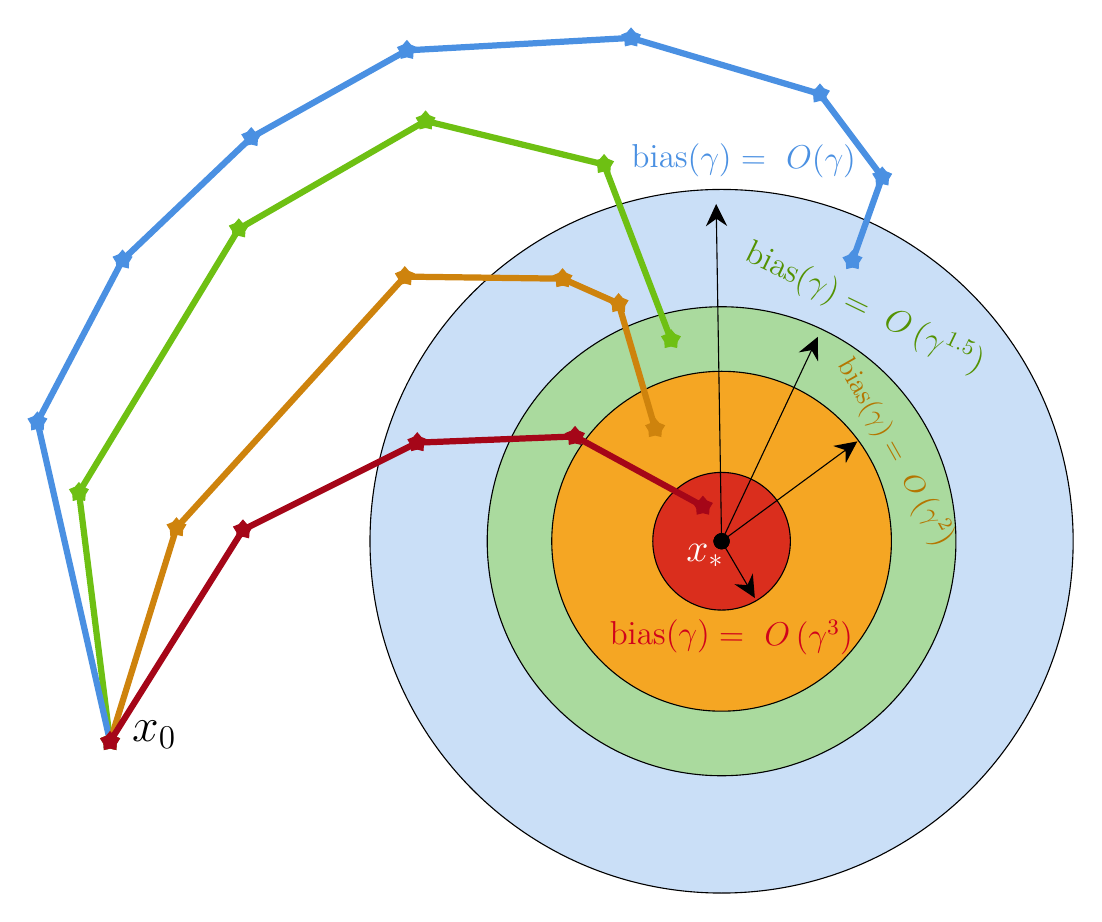
\begin{tikzpicture}[x=0.75pt,y=0.75pt,yscale=-1,xscale=1]


%Shape: Ellipse [id:dp7329906304802944] 
\draw  [fill={rgb, 255:red, 74; green, 144; blue, 226 }  ,fill opacity=0.29 ] (481.22,393.5) .. controls (481.22,299.89) and (557.06,224) .. (650.61,224) .. controls (744.16,224) and (820,299.89) .. (820,393.5) .. controls (820,487.11) and (744.16,563) .. (650.61,563) .. controls (557.06,563) and (481.22,487.11) .. (481.22,393.5) -- cycle ;
%Shape: Ellipse [id:dp14673386188875415] 
\draw  [fill={rgb, 255:red, 126; green, 211; blue, 33 }  ,fill opacity=0.41 ] (537.7,393.5) .. controls (537.7,331.1) and (588.25,280.52) .. (650.61,280.52) .. controls (712.97,280.52) and (763.52,331.1) .. (763.52,393.5) .. controls (763.52,455.9) and (712.97,506.48) .. (650.61,506.48) .. controls (588.25,506.48) and (537.7,455.9) .. (537.7,393.5) -- cycle ;
%Shape: Ellipse [id:dp3138874134344609] 
\draw  [fill={rgb, 255:red, 245; green, 166; blue, 35 }  ,fill opacity=1 ] (568.79,393.5) .. controls (568.79,348.28) and (605.42,311.62) .. (650.61,311.62) .. controls (695.8,311.62) and (732.44,348.28) .. (732.44,393.5) .. controls (732.44,438.72) and (695.8,475.38) .. (650.61,475.38) .. controls (605.42,475.38) and (568.79,438.72) .. (568.79,393.5) -- cycle ;
%Shape: Ellipse [id:dp6951380714624634] 
\draw  [fill={rgb, 255:red, 208; green, 2; blue, 27 }  ,fill opacity=0.73 ] (617.47,393.5) .. controls (617.47,375.18) and (632.31,360.34) .. (650.61,360.34) .. controls (668.91,360.34) and (683.75,375.18) .. (683.75,393.5) .. controls (683.75,411.82) and (668.91,426.66) .. (650.61,426.66) .. controls (632.31,426.66) and (617.47,411.82) .. (617.47,393.5) -- cycle ;

% =============== COLORED POLYLINES WITH STARS ===============

% Green path
\draw [color={rgb, 255:red, 110; green, 192; blue, 19 }, line width=2.25]
  (356,490) -- (341,370) -- (418,243) -- (508,191) -- (594,212) -- (626.22,296.33);
\foreach \p in {(356,490),(341,370),(418,243),(508,191),(594,212),(626.22,296.33)}{
  \node[star, star points=5, draw={rgb,255:red,110; green,192; blue,19},
        fill={rgb,255:red,110; green,192; blue,19}, minimum size=7pt, inner sep=0pt] at \p {};
}

% Blue path
\draw [color={rgb, 255:red, 74; green, 144; blue, 226 }, line width=2.25]
  (356,490) -- (321,336) -- (362,258) -- (424,199) -- (499,157) -- (607,151)
  -- (698,178) -- (728,218) -- (713.68,258.29);
\foreach \p in {  (356,490) , (321,336) , (362,258) , (424,199) , (499,157) , (607,151)
  , (698,178) , (728,218) , (713.68,258.29)}{
  \node[star, star points=5, draw={rgb,255:red,74; green,144; blue,226},
        fill={rgb,255:red,74; green,144; blue,226}, minimum size=7pt, inner sep=0pt] at \p {};
}

% Orange path
\draw [color={rgb, 255:red, 206; green, 131; blue, 13 }, line width=2.25]
  (356,490) -- (388,387) -- (498,266) -- (574,267) -- (601,279) -- (618.6,339.2);
\foreach \p in {(356,490),(388,387),(498,266),(574,267),(601,279),(618.6,339.2)}{
  \node[star, star points=5, draw={rgb,255:red,206; green,131; blue,13},
        fill={rgb,255:red,206; green,131; blue,13}, minimum size=7pt, inner sep=0pt] at \p {};
}

% Red path
\draw [color={rgb, 255:red, 165; green, 6; blue, 24 }, line width=2.25]
  (356,490) -- (420,388) -- (504,346) -- (580,343) -- (641.61,376.61);
\foreach \p in {(356,490),(420,388),(504,346),(580,343),(641.61,376.61)}{
  \node[star, star points=5, draw={rgb,255:red,165; green,6; blue,24},
        fill={rgb,255:red,165; green,6; blue,24}, minimum size=7pt, inner sep=0pt] at \p {};
}

% =============================================================
%
%% Text Node
%\draw (632.38,393.8) node [anchor=north west][inner sep=0.75pt]  [font=\Large,color={rgb, 255:red, 255; green, 255; blue, 255 }  ,opacity=1 ]  {$x_{*}$};
%% Text Node
%\draw (606.03,200.22) node [anchor=north west][inner sep=0.75pt]  [font=\Large,color={rgb, 255:red, 74; green, 144; blue, 226 }  ,opacity=1 ,rotate=-0.45]  {$\mathrm{bias}( \gamma ) =\ \mathcal{O}\left( \gamma \right)$};
%% Text Node
%\draw (671.93,254.71) node [anchor=north west][inner sep=0.75pt]  [font=\Large,color={rgb, 255:red, 100; green, 172; blue, 43 },opacity=1 ,rotate=-25.81]  {$\mathrm{bias}( \gamma ) =\ \mathcal{O}\left( \gamma ^{1.5}\right)$};
%% Text Node
%\draw (598.56,429.08) node [anchor=north west][inner sep=0.75pt]  [font=\Large,color={rgb, 255:red, 208; green, 2; blue, 27 }  ,opacity=1 ,rotate=-0.61]  {$\mathrm{bias}( \gamma ) =\ \mathcal{O}\left( \gamma ^{3}\right)$};
%% Text Node
%\draw (720.43,309.21) node [anchor=north west][inner sep=0.75pt]  [font=\large,color={rgb, 255:red, 231; green, 151; blue, 19 }  ,opacity=1 ,rotate=-60.58]  {$\mathrm{bias}( \gamma ) =\ \mathcal{O}\left( \gamma ^{2}\right)$};
%% Text Node
%\draw (372.38,478.8) node [anchor=north west][inner sep=0.75pt]  [font=\Large,color={rgb, 255:red, 0; green, 0; blue, 0 }  ,opacity=1 ]  {$x_{0}$};

% Text Node
\draw (632.38,393.8) node [anchor=north west][inner sep=0.75pt]  [font=\Large,color={rgb, 255:red, 255; green, 255; blue, 255 }  ,opacity=1 ]  {$x_{*}$};
% Text Node
\draw (606.03,200.22) node [anchor=north west][inner sep=0.75pt]  [font=\large,color={rgb, 255:red, 74; green, 144; blue, 226 }  ,opacity=1 ,rotate=-0.45]  {$\mathrm{bias}( \gamma ) =\ O( \gamma )$};
% Text Node
\draw (665.93,244.71) node [anchor=north west][inner sep=0.75pt]  [font=\large,color={rgb, 255:red, 83; green, 146; blue, 2 }  ,opacity=1 ,rotate=-25.81]  {$\mathrm{bias}( \gamma ) =\ O\left( \gamma ^{1.5}\right)$};
% Text Node
\draw (595.56,429.08) node [anchor=north west][inner sep=0.75pt]  [font=\large,color={rgb, 255:red, 208; green, 2; blue, 27 }  ,opacity=1 ,rotate=-0.61]  {$\mathrm{bias}( \gamma ) =\ O\left( \gamma ^{3}\right)$};
% Text Node
\draw (716.43,301.21) node [anchor=north west][inner sep=0.75pt]  [font=\normalsize,color={rgb, 255:red, 180; green, 117; blue, 0 }  ,opacity=1 ,rotate=-60.58]  {$\mathrm{bias}( \gamma ) =\ O\left( \gamma ^{2}\right)$};
% Text Node
\draw (365.38,478.8) node [anchor=north west][inner sep=0.75pt]  [font=\LARGE,color={rgb, 255:red, 0; green, 0; blue, 0 }  ,opacity=1 ]  {$x_{0}$};

%Straight Lines [id:da7873343135782715] 
\draw    (650.61,393.5) -- (648.05,234) ;
\draw [shift={(648,231)}, rotate = 89.08] [fill={rgb, 255:red, 0; green, 0; blue, 0 }  ][line width=0.08]  [draw opacity=0] (10.72,-5.15) -- (0,0) -- (10.72,5.15) -- (7.12,0) -- cycle    ;
\draw [shift={(650.61,393.5)}, rotate = 269.08] [color={rgb, 255:red, 0; green, 0; blue, 0 }  ][fill={rgb, 255:red, 0; green, 0; blue, 0 }  ][line width=0.75]      (0, 0) circle [x radius= 3.35, y radius= 3.35]   ;
%Straight Lines [id:da8747548930371518] 
\draw    (650.61,393.5) -- (695.72,297.71) ;
\draw [shift={(697,295)}, rotate = 115.22] [fill={rgb, 255:red, 0; green, 0; blue, 0 }  ][line width=0.08]  [draw opacity=0] (10.72,-5.15) -- (0,0) -- (10.72,5.15) -- (7.12,0) -- cycle    ;
\draw [shift={(650.61,393.5)}, rotate = 295.22] [color={rgb, 255:red, 0; green, 0; blue, 0 }  ][fill={rgb, 255:red, 0; green, 0; blue, 0 }  ][line width=0.75]      (0, 0) circle [x radius= 3.35, y radius= 3.35]   ;
%Straight Lines [id:da18150789044644122] 
\draw    (650.61,393.5) -- (713.61,347.16) ;
\draw [shift={(716.03,345.38)}, rotate = 143.66] [fill={rgb, 255:red, 0; green, 0; blue, 0 }  ][line width=0.08]  [draw opacity=0] (10.72,-5.15) -- (0,0) -- (10.72,5.15) -- (7.12,0) -- cycle    ;
\draw [shift={(650.61,393.5)}, rotate = 323.66] [color={rgb, 255:red, 0; green, 0; blue, 0 }  ][fill={rgb, 255:red, 0; green, 0; blue, 0 }  ][line width=0.75]      (0, 0) circle [x radius= 3.35, y radius= 3.35]   ;
%Straight Lines [id:da6863210759512379] 
\draw    (650.61,393.5) -- (665.12,418.22) ;
\draw [shift={(666.64,420.81)}, rotate = 239.59] [fill={rgb, 255:red, 0; green, 0; blue, 0 }  ][line width=0.08]  [draw opacity=0] (10.72,-5.15) -- (0,0) -- (10.72,5.15) -- (7.12,0) -- cycle    ;
\draw [shift={(650.61,393.5)}, rotate = 59.59] [color={rgb, 255:red, 0; green, 0; blue, 0 }  ][fill={rgb, 255:red, 0; green, 0; blue, 0 }  ][line width=0.75]      (0, 0) circle [x radius= 3.35, y radius= 3.35]   ;



% % Central point and labels
% \draw (632.38,393.8) node [anchor=north west][inner sep=0.75pt] [font=\large,color=white] {$x_{*}$};
% \draw (606.03,200.22) node [anchor=north west][font=\footnotesize,color={rgb, 255:red, 74; green, 144; blue, 226 }] {$\mathrm{bias}( \gamma ) =\ O( \gamma )$};
% \draw (671.93,254.71) node [anchor=north west][font=\footnotesize,color={rgb, 255:red, 126; green, 211; blue, 33 }] {$\mathrm{bias}( \gamma ) =\ O\!\left( \gamma ^{1.5}\right)$};
% \draw (598.56,429.08) node [anchor=north west][font=\footnotesize,color={rgb, 255:red, 208; green, 2; blue, 27 }] {$\mathrm{bias}( \gamma ) =\ O\!\left( \gamma ^{3}\right)$};
% \draw (720.43,309.21) node [anchor=north west][font=\footnotesize,color={rgb, 255:red, 231; green, 151; blue, 19 }] {$\mathrm{bias}( \gamma ) =\ O\!\left( \gamma ^{2}\right)$};
% \draw (372.38,478.8) node [anchor=north west][font=\large,color=black] {$x_{0}$};

\end{tikzpicture}}
        %\caption*{(b) Asymptotic neighborhood of $x_k$.}
    \end{minipage}
    \caption{Illustration of bias behavior. 
    \textbf{(a)} Example on a quadratic VIP with $F(x)=\tfrac{1}{N}\sum x^\top A x$ for $N=1000$. 
    Already after the second epoch, the methods clearly separate: 
    \textcolor{blue}{SGD}, \textcolor{green}{\RRresh}, \textcolor{orange}{\RRrom}, 
    and \textcolor{red}{\RRresh$\oplus$\RRrom}. 
    \textbf{(b)} Decomposition of the iterates as 
    $x_k = x_* + C e^{-k} + \text{bias}_{\text{method}}(\gamma)$, 
    illustrating how the asymptotic neighborhood depends on the bias term.}
\end{figure}

\newpage

\begin{figure}[ht]
    \centering
    \scalebox{0.65}{

\tikzset{every picture/.style={line width=0.75pt}} %set default line width to 0.75pt        

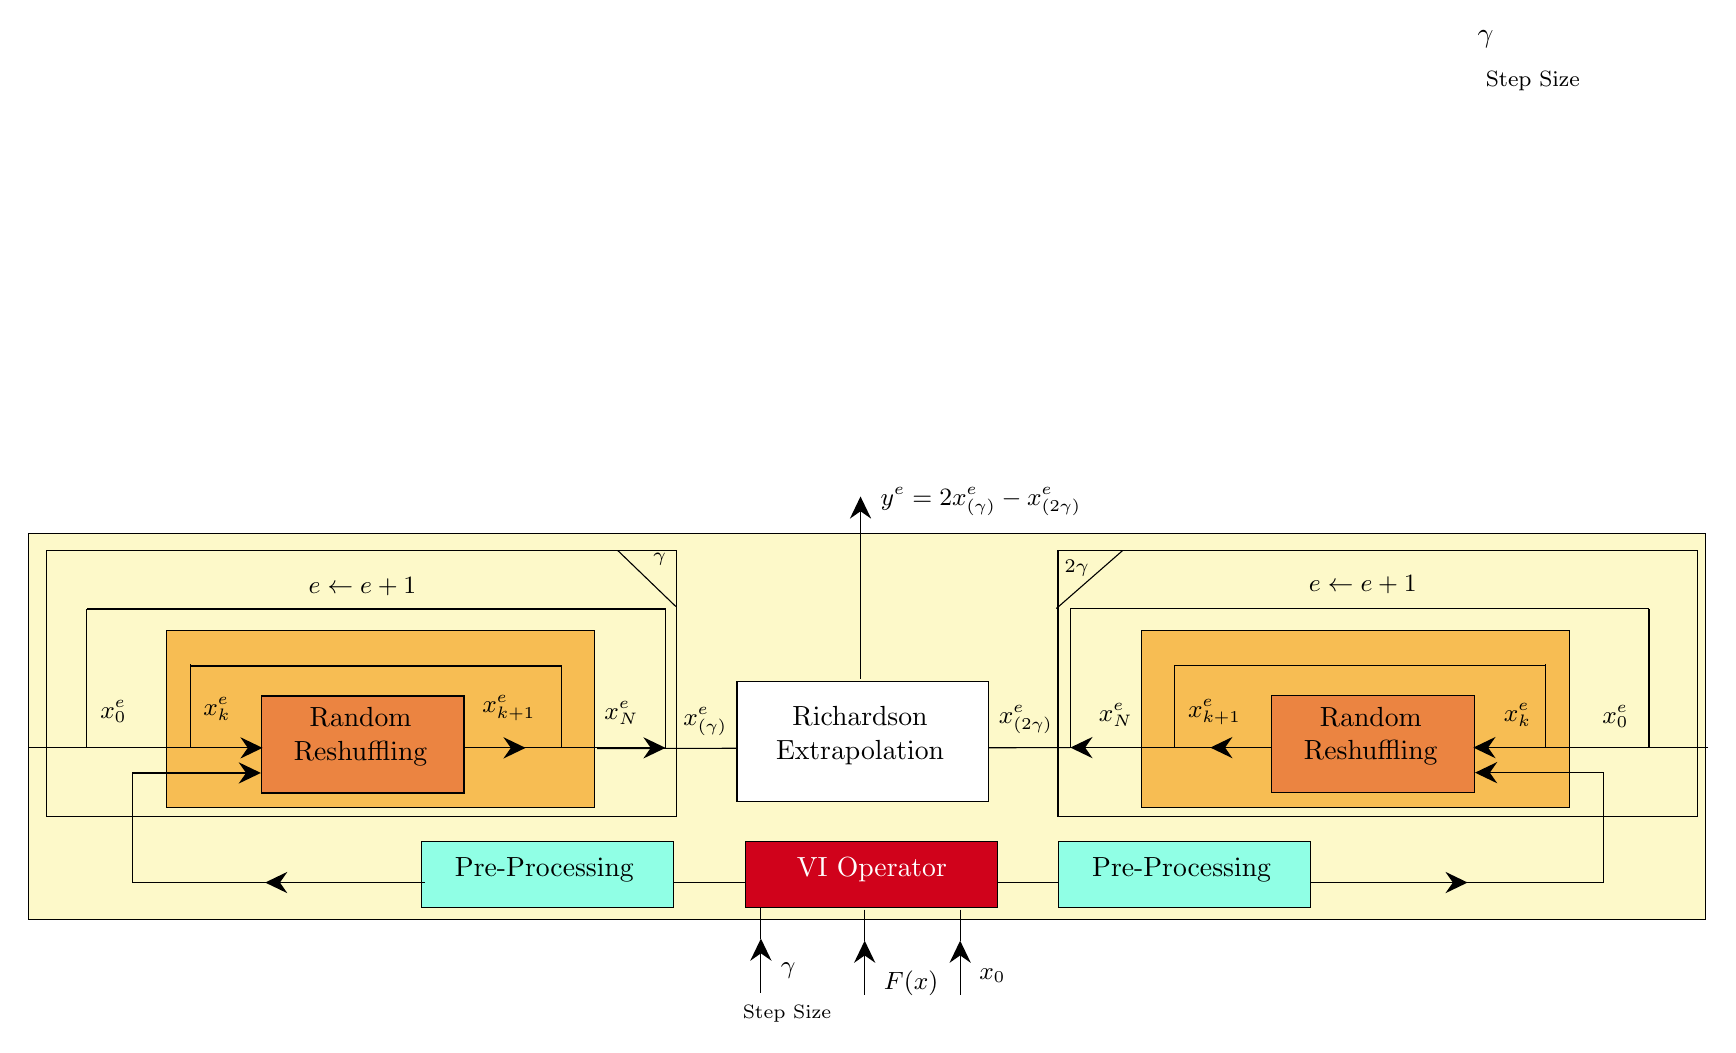
\begin{tikzpicture}[x=0.75pt,y=0.75pt,yscale=-1,xscale=1]
%uncomment if require: \path (0,711); %set diagram left start at 0, and has height of 711

%Shape: Rectangle [id:dp7167201570186642] 
\draw  [fill={rgb, 255:red, 248; green, 231; blue, 28 }  ,fill opacity=0.24 ] (24,362) -- (832,362) -- (832,548) -- (24,548) -- cycle ;
%Straight Lines [id:da5348252051360501] 
\draw    (215.16,530) -- (642,530) ;
%Straight Lines [id:da5870165356755055] 
\draw    (642,530) -- (783.02,530) ;
\draw [shift={(717.51,530)}, rotate = 180] [fill={rgb, 255:red, 0; green, 0; blue, 0 }  ][line width=0.08]  [draw opacity=0] (10.72,-5.15) -- (0,0) -- (10.72,5.15) -- (7.12,0) -- cycle    ;
%Shape: Rectangle [id:dp22967037843062987] 
\draw  [fill={rgb, 255:red, 245; green, 166; blue, 35 }  ,fill opacity=0.71 ] (90.45,408.54) -- (296.62,408.54) -- (296.62,493.84) -- (90.45,493.84) -- cycle ;
%Straight Lines [id:da17785199775015115] 
\draw    (74.14,477.2) -- (133.09,477.2) ;
\draw [shift={(136.09,477.2)}, rotate = 180] [fill={rgb, 255:red, 0; green, 0; blue, 0 }  ][line width=0.08]  [draw opacity=0] (10.72,-5.15) -- (0,0) -- (10.72,5.15) -- (7.12,0) -- cycle    ;
%Shape: Rectangle [id:dp2742561061453428] 
\draw  [fill={rgb, 255:red, 208; green, 2; blue, 27 }  ,fill opacity=0.3 ] (136.49,440.15) -- (233.94,440.15) -- (233.94,486.86) -- (136.49,486.86) -- cycle ;

%Straight Lines [id:da09921992906541832] 
\draw    (102.26,465.12) -- (133.9,465.12) ;
\draw [shift={(136.9,465.12)}, rotate = 180] [fill={rgb, 255:red, 0; green, 0; blue, 0 }  ][line width=0.08]  [draw opacity=0] (10.72,-5.15) -- (0,0) -- (10.72,5.15) -- (7.12,0) -- cycle    ;
%Straight Lines [id:da337709340044827] 
\draw    (234.35,465.12) -- (260.64,465.12) ;
\draw [shift={(263.64,465.12)}, rotate = 180] [fill={rgb, 255:red, 0; green, 0; blue, 0 }  ][line width=0.08]  [draw opacity=0] (10.72,-5.15) -- (0,0) -- (10.72,5.15) -- (7.12,0) -- cycle    ;
%Straight Lines [id:da8354383452527102] 
\draw    (240.28,465.12) -- (281.06,465.12) ;
%Straight Lines [id:da8152793732524597] 
\draw    (281.06,465.12) -- (281.06,425.65) ;
%Straight Lines [id:da7570544004782095] 
\draw    (102.26,465.12) -- (102.26,424.85) ;
%Straight Lines [id:da4721478714710243] 
\draw    (281.06,425.65) -- (102.26,425.65) ;
%Straight Lines [id:da3188806653380546] 
\draw    (281.06,465.12) -- (328.05,465.12) ;
\draw [shift={(331.05,465.12)}, rotate = 180] [fill={rgb, 255:red, 0; green, 0; blue, 0 }  ][line width=0.08]  [draw opacity=0] (10.72,-5.15) -- (0,0) -- (10.72,5.15) -- (7.12,0) -- cycle    ;
%Straight Lines [id:da5695989834818472] 
\draw    (52.27,465.12) -- (102.26,465.12) ;
%Straight Lines [id:da005449392824766197] 
\draw    (52.27,465.12) -- (52.27,398.2) ;
%Straight Lines [id:da5087383745711406] 
\draw    (331.05,465.12) -- (331.05,398.2) ;
%Straight Lines [id:da7805722702952284] 
\draw    (331.05,398.2) -- (52.27,398.2) ;
%Straight Lines [id:da42790020085683145] 
\draw    (52.27,465.12) -- (24.08,465.12) ;
%Shape: Rectangle [id:dp8867101993788168] 
\draw  [fill={rgb, 255:red, 245; green, 166; blue, 35 }  ,fill opacity=0.71 ] (766.71,408.41) -- (560.54,408.41) -- (560.54,493.71) -- (766.71,493.71) -- cycle ;
%Straight Lines [id:da45046936384949954] 
\draw    (783.02,477.06) -- (724.07,477.06) ;
\draw [shift={(721.07,477.06)}, rotate = 360] [fill={rgb, 255:red, 0; green, 0; blue, 0 }  ][line width=0.08]  [draw opacity=0] (10.72,-5.15) -- (0,0) -- (10.72,5.15) -- (7.12,0) -- cycle    ;
%Shape: Rectangle [id:dp8984113920591881] 
\draw  [fill={rgb, 255:red, 208; green, 2; blue, 27 }  ,fill opacity=0.3 ] (623.21,440.01) -- (720.67,440.01) -- (720.67,486.73) -- (623.21,486.73) -- cycle ;

%Straight Lines [id:da49889800256014705] 
\draw    (754.89,464.98) -- (723.26,464.98) ;
\draw [shift={(720.26,464.98)}, rotate = 360] [fill={rgb, 255:red, 0; green, 0; blue, 0 }  ][line width=0.08]  [draw opacity=0] (10.72,-5.15) -- (0,0) -- (10.72,5.15) -- (7.12,0) -- cycle    ;
%Straight Lines [id:da31365561028594713] 
\draw    (622.81,464.98) -- (596.52,464.98) ;
\draw [shift={(593.52,464.98)}, rotate = 360] [fill={rgb, 255:red, 0; green, 0; blue, 0 }  ][line width=0.08]  [draw opacity=0] (10.72,-5.15) -- (0,0) -- (10.72,5.15) -- (7.12,0) -- cycle    ;
%Straight Lines [id:da9666480403965403] 
\draw    (616.88,464.98) -- (576.1,464.98) ;
%Straight Lines [id:da6870758288531431] 
\draw    (576.1,464.98) -- (576.1,425.52) ;
%Straight Lines [id:da13859487218454614] 
\draw    (754.89,464.98) -- (754.89,424.71) ;
%Straight Lines [id:da30734305051591637] 
\draw    (576.1,425.52) -- (754.89,425.52) ;
%Straight Lines [id:da11442520008239165] 
\draw    (576.1,464.98) -- (529.1,464.98) ;
\draw [shift={(526.1,464.98)}, rotate = 360] [fill={rgb, 255:red, 0; green, 0; blue, 0 }  ][line width=0.08]  [draw opacity=0] (10.72,-5.15) -- (0,0) -- (10.72,5.15) -- (7.12,0) -- cycle    ;
%Straight Lines [id:da11238862430956253] 
\draw    (804.89,464.98) -- (754.89,464.98) ;
%Straight Lines [id:da3927723255927097] 
\draw    (804.89,464.98) -- (804.89,398.06) ;
%Straight Lines [id:da17493801390941033] 
\draw    (526.1,464.98) -- (526.1,398.06) ;
%Straight Lines [id:da38944767089549004] 
\draw    (526.1,398.06) -- (804.89,398.06) ;
%Straight Lines [id:da5789729604768556] 
\draw    (298.12,465.45) -- (526.1,464.98) ;
%Straight Lines [id:da5056140478751464] 
\draw    (804.89,464.98) -- (833.08,464.98) ;
%Shape: Rectangle [id:dp6283534568839406] 
\draw   (33,369.87) -- (336.12,369.87) -- (336.12,498) -- (33,498) -- cycle ;
%Straight Lines [id:da7766228141098565] 
\draw    (425,347) -- (425,432) ;
\draw [shift={(425,344)}, rotate = 90] [fill={rgb, 255:red, 0; green, 0; blue, 0 }  ][line width=0.08]  [draw opacity=0] (10.72,-5.15) -- (0,0) -- (10.72,5.15) -- (7.12,0) -- cycle    ;
%Shape: Rectangle [id:dp0677493839993355] 
\draw   (520.12,369.87) -- (828.12,369.87) -- (828.12,498) -- (520.12,498) -- cycle ;
%Shape: Rectangle [id:dp014110378228816445] 
\draw  [fill={rgb, 255:red, 255; green, 255; blue, 255 }  ,fill opacity=1 ] (365.5,433) -- (486.5,433) -- (486.5,491) -- (365.5,491) -- cycle ;

%Shape: Rectangle [id:dp8640505621986145] 
\draw  [fill={rgb, 255:red, 144; green, 255; blue, 229 }  ,fill opacity=1 ] (213.49,510.15) -- (335,510.15) -- (335,542) -- (213.49,542) -- cycle ;

%Shape: Rectangle [id:dp11807891437834184] 
\draw  [fill={rgb, 255:red, 144; green, 255; blue, 229 }  ,fill opacity=1 ] (520.49,510.15) -- (642,510.15) -- (642,542) -- (520.49,542) -- cycle ;

%Straight Lines [id:da6023255336667221] 
\draw    (74.14,477.2) -- (74.14,530) ;
%Straight Lines [id:da047541439752831094] 
\draw    (783.02,477.06) -- (783.02,529.87) ;
%Straight Lines [id:da38440122612945915] 
\draw    (74.14,530) -- (215.16,530) ;
\draw [shift={(138.15,530)}, rotate = 0] [fill={rgb, 255:red, 0; green, 0; blue, 0 }  ][line width=0.08]  [draw opacity=0] (10.72,-5.15) -- (0,0) -- (10.72,5.15) -- (7.12,0) -- cycle    ;
%Shape: Rectangle [id:dp7774128051215404] 
\draw  [fill={rgb, 255:red, 208; green, 2; blue, 27 }  ,fill opacity=1 ] (369.49,510.15) -- (491,510.15) -- (491,542) -- (369.49,542) -- cycle ;
%Straight Lines [id:da048020115234232885] 
\draw    (308,370) -- (336,397) ;
%Straight Lines [id:da22128359563915156] 
\draw    (551.33,370) -- (519.33,398) ;
%Straight Lines [id:da4178126076311651] 
\draw    (427,561) -- (427,584) ;
\draw [shift={(427,558)}, rotate = 90] [fill={rgb, 255:red, 0; green, 0; blue, 0 }  ][line width=0.08]  [draw opacity=0] (10.72,-5.15) -- (0,0) -- (10.72,5.15) -- (7.12,0) -- cycle    ;
%Straight Lines [id:da2712874934584891] 
\draw    (427,543) -- (427,558) ;
%Straight Lines [id:da22537158810197067] 
\draw    (377,560) -- (377,583) ;
\draw [shift={(377,557)}, rotate = 90] [fill={rgb, 255:red, 0; green, 0; blue, 0 }  ][line width=0.08]  [draw opacity=0] (10.72,-5.15) -- (0,0) -- (10.72,5.15) -- (7.12,0) -- cycle    ;
%Straight Lines [id:da17343167705220275] 
\draw    (377,542) -- (377,557) ;
%Straight Lines [id:da5797829827731849] 
\draw    (473,561) -- (473,584) ;
\draw [shift={(473,558)}, rotate = 90] [fill={rgb, 255:red, 0; green, 0; blue, 0 }  ][line width=0.08]  [draw opacity=0] (10.72,-5.15) -- (0,0) -- (10.72,5.15) -- (7.12,0) -- cycle    ;
%Straight Lines [id:da3209997322336591] 
\draw    (473,543) -- (473,558) ;

% Text Node
\draw (147.12,444.5) node [anchor=north west][inner sep=0.75pt]   [align=left] {\begin{minipage}[lt]{53.57pt}\setlength\topsep{0pt}
\begin{center}
Random \\Reshuffling
\end{center}

\end{minipage}};
% Text Node
\draw (382,444) node [anchor=north west][inner sep=0.75pt]   [align=left] {\begin{minipage}[lt]{62.26pt}\setlength\topsep{0pt}
\begin{center}
Richardson\\Extrapolation
\end{center}

\end{minipage}};
% Text Node
\draw (721,118.4) node [anchor=north west][inner sep=0.75pt]    {$\gamma $};
% Text Node
\draw (725,138) node [anchor=north west][inner sep=0.75pt]  [font=\footnotesize] [align=left] {Step Size\\};
% Text Node
\draw (633.84,444.37) node [anchor=north west][inner sep=0.75pt]   [align=left] {\begin{minipage}[lt]{53.57pt}\setlength\topsep{0pt}
\begin{center}
Random \\Reshuffling
\end{center}

\end{minipage}};
% Text Node
\draw (107.08,439.73) node [anchor=north west][inner sep=0.75pt]  [font=\small]  {$x_{k}^{e}$};
% Text Node
\draw (241.59,438.5) node [anchor=north west][inner sep=0.75pt]  [font=\small]  {$x_{k+1}^{e}$};
% Text Node
\draw (300.38,441.53) node [anchor=north west][inner sep=0.75pt]  [font=\small]  {$x_{N}^{e}$};
% Text Node
\draw (57.55,441.12) node [anchor=north west][inner sep=0.75pt]  [font=\small]  {$x_{0}^{e}$};
% Text Node
\draw (157.77,381.59) node [anchor=north west][inner sep=0.75pt]  [font=\small]  {$e\leftarrow e+1$};
% Text Node
\draw (522.12,373.27) node [anchor=north west][inner sep=0.75pt]  [font=\scriptsize]  {$2\gamma $};
% Text Node
\draw (581.57,440.59) node [anchor=north west][inner sep=0.75pt]  [font=\small]  {$x_{k+1}^{e}$};
% Text Node
\draw (733.67,442.41) node [anchor=north west][inner sep=0.75pt]  [font=\small]  {$x_{k}^{e}$};
% Text Node
\draw (538.59,442.4) node [anchor=north west][inner sep=0.75pt]  [font=\small]  {$x_{N}^{e}$};
% Text Node
\draw (781.21,443.59) node [anchor=north west][inner sep=0.75pt]  [font=\small]  {$x_{0}^{e}$};
% Text Node
\draw (433.38,338.53) node [anchor=north west][inner sep=0.75pt]  [font=\small]  {$y^{e} =2x_{( \gamma )}^{e} -x_{( 2\gamma )}^{e}$};
% Text Node
\draw (639.77,380.59) node [anchor=north west][inner sep=0.75pt]  [font=\small]  {$e\leftarrow e+1$};
% Text Node
\draw (338.38,444.53) node [anchor=north west][inner sep=0.75pt]  [font=\small]  {$x_{( \gamma )}^{e}$};
% Text Node
\draw (490.38,443.53) node [anchor=north west][inner sep=0.75pt]  [font=\small]  {$x_{( 2\gamma )}^{e}$};
% Text Node
\draw (223.12,516.5) node [anchor=north west][inner sep=0.75pt]   [align=left] {\begin{minipage}[lt]{72.45pt}\setlength\topsep{0pt}
\begin{center}
Pre-Processing
\end{center}

\end{minipage}};
% Text Node
\draw (323.83,369.96) node [anchor=north west][inner sep=0.75pt]  [font=\scriptsize]  {$\gamma $};
% Text Node
\draw (530.12,516.5) node [anchor=north west][inner sep=0.75pt]   [align=left] {\begin{minipage}[lt]{72.45pt}\setlength\topsep{0pt}
\begin{center}
Pre-Processing
\end{center}

\end{minipage}};
% Text Node
\draw (382.12,516.5) node [anchor=north west][inner sep=0.75pt]  [color={rgb, 255:red, 255; green, 255; blue, 255 }  ,opacity=1 ] [align=left] {\begin{minipage}[lt]{63.95pt}\setlength\topsep{0pt}
\begin{center}
 \ \ VI Operator
\end{center}

\end{minipage}};
% Text Node
\draw (435,571.4) node [anchor=north west][inner sep=0.75pt]  [font=\small]  {$F( x)$};
% Text Node
\draw (385.38,567.53) node [anchor=north west][inner sep=0.75pt]  [font=\small]  {$\gamma $};
% Text Node
\draw (367,588) node [anchor=north west][inner sep=0.75pt]  [font=\scriptsize] [align=left] {Step Size};
% Text Node
\draw (481,570.4) node [anchor=north west][inner sep=0.75pt]  [font=\small]  {$x_{0}$};


\end{tikzpicture}
}
    \caption{Algorithmic Model of \RRresh$\oplus$\RRrom}
\end{figure}

%To the best of our knowledge, this work is the first to demonstrate that these heuristics can be synthesized into a principled algorithmic framework, yielding a composite bias reduction unattainable by any of them in isolation.



% Concretely, whenever the bias expands as $\text{bias}_{}(\gamma) = \Delta \gamma + O(\gamma^{\kappa})$ for some $\kappa>1$,
% then if 
%         $x_{\infty}^{\gamma} - x^* = \Delta\dot\gamma + O(\gamma^{\kappa}), \quad x_{\infty}^{2\gamma} - x^* = \Delta\dot 2\gamma + O(\gamma^{\kappa})$ then extrapolating yields
% $        2x_{\infty}^{\gamma}- x_{\infty}^{2\gamma} - x^* = \cancel{2\Delta \gamma} - \cancel{2\Delta \gamma} + \mathcal{O}\left(\gamma^{\kappa}\right) = \mathcal{O}\left(\gamma^{\kappa}\right) \nonumber
% $

% \begin{eqnarray}
%         x_{\infty}^{\gamma} - x^* = \Delta\dot\gamma + O(\gamma^{\kappa}), \quad x_{\infty}^{2\gamma} - x^* = \Delta\dot 2\gamma + O(\gamma^{\kappa})\\
%         2x_{\infty}^{\gamma}- x_{\infty}^{2\gamma} - x^* = \cancel{2\Delta \gamma} - \cancel{2\Delta \gamma} + \mathcal{O}\left(\gamma^{\kappa}\right) = \mathcal{O}\left(\gamma^{\kappa}\right) \nonumber
% \end{eqnarray}

% \newpage

% Orthogonal to the above, another classical debiasing technique has recently gained traction in stochastic optimization: Richardson–Romberg (RR) extrapolation. Originally developed in numerical analysis to improve the accuracy of discretization schemes [Hildebrand, 1987], RR operates by combining approximations with different step sizes so as to cancel the leading term in the error expansion. The one-step version was introduced to reduce discretization error in Euler schemes for stochastic differential equations [Talay & Tubaro, 1990], later extended to non-smooth settings [Bally & Talay, 1996] and multistep discretizations [Pages, 2007].

% The same idea can be applied to constant-step stochastic gradient methods: if the stationary bias admits an expansion of the form
% x_{\infty}^{\gamma} - x^* = \Delta \gamma + O(\gamma^{\kappa}),
% \quad
% x_{\infty}^{2\gamma} - x^* = 2\Delta \gamma + O(\gamma^{\kappa}),
% then extrapolating yields
% 2x_{\infty}^{\gamma} - x_{\infty}^{2\gamma} - x^*
% = \cancel{2\Delta \gamma} - \cancel{2\Delta \gamma} + O(\gamma^{\kappa})
% = O(\gamma^{\kappa}),
% thereby eliminating the dominant bias term. This simple yet powerful idea has motivated a growing line of work applying RR to stochastic approximation methods, including SGD [Durmus et al., 2016; Dieuleveut et al., 2020; Merad & Gaïffas, 2023; Huo et al., 2024a], Q-learning, and other single- and two-timescale algorithms [Allmeier & Gast, 2024; Zhang & Xie, 2024; Huo et al., 2024a; Kwon et al., 2024].

% Despite this progress, the theoretical understanding of RR in the context of stochastic VIs remains nascent. Prior work has either assumed unbiased stochastic oracles [Bach], or leveraged specific structural properties of the noise [Vlatakis et al.]. Thus, while RR has proven effective in practice and across related stochastic approximation problems, its guarantees for general variational inequalities are still incomplete.

% \newpage


% Orthogonal to the above, there is another folkore from numerical analysis debiasing technique that has become popular in the field of stochastic VIs, the Richardson - Romberg extrapolation. Richardson requires a more refined analysis of the bias of the method, decomposing into a dominant term and some higher order ones, resulting in $\text{bias}_{}(\gamma) = \Delta \gamma + O(\gamma^{\kappa})$
% \begin{eqnarray}
%         x_{\infty}^{\gamma} - x^* = \Delta\dot\gamma + O(\gamma^{\kappa}), \quad x_{\infty}^{2\gamma} - x^* = \Delta\dot 2\gamma + O(\gamma^{\kappa})\\
%         2x_{\infty}^{\gamma}- x_{\infty}^{2\gamma} - x^* = \cancel{2\Delta \gamma} - \cancel{2\Delta \gamma} + \mathcal{O}\left(\gamma^{\kappa}\right) = \mathcal{O}\left(\gamma^{\kappa}\right) \nonumber
% \end{eqnarray}
% Despite the simplicity of the method, the theoretical understanding is nascent. Papers for Richardson explaining the method in minimization (cite Bach) and in VI (Vlatakis). The first analyzed the method with unbiased stochastic oracles, while the second were utilizing specific structure of the noise. 

% Richardson-Romberg (RR) extrapolation is a technique used to improve the accuracy of numerical approximations (Hildebrand, 1987), such as those from numerical differentiation or integration. It involves using approximations with different step sizes and then extrapolating to reduce the error, typically by removing the leading term in the error expansion. The one-step RR extrapolation was introduced to reduce the discretization error induced by an Euler scheme to simulate stochastic differential equation in Talay & Tubaro (1990), and later generalized for non-smooth functions in Bally & Talay (1996). This technique was extended using multistep discretizations in Page`s (2007). RR extrapolation have been applied to Stochastic Gradient Descent (SGD) methods in Durmus et al. (2016), Dieuleveut et al. (2020), Merad & Ga ̈ıffas (2023) and Huo et al. (2024a), to improve convergence and reduce error in optimization problems, particularly when dealing with noisy or high-variance gradient estimates. Recent papers (Allmeier & Gast, 2024; Zhang & Xie, 2024; Huo et al., 2024a; Kwon et al., 2024) consider applications of RR to different stochastic approximation problems with constant step-size, including Q-learning, and single- and two-timescale stochastic approximation.


% To address this issue, practitioners often turn to debiasing heuristics. One such technique, widely adopted in stochastic optimization, is \emph{random reshuffling} (RR), or \emph{without-replacement} sampling, where each data point is used exactly once per epoch. Unlike the classical \emph{with-replacement} variant of SGD—where samples are drawn independently and some may be revisited while others are skipped. RR eliminates this redundancy by enforcing a full pass over the dataset in a random order, closely matching how large-scale training is implemented in practice.
% Despite the dependence it induces across samples within an epoch, recent work has established faster convergence guarantees for RR in both minimization and VIPs \cite{Ahn et al., 2020; Gürbüzbalaban et al., 2021; Mishchenko et al., 2020a; Cai et al., 2023}. Beyond these rate improvements, RR has also been shown to reduce the stationary bias of constant-step methods from $O(\gamma)$ to $O(\gamma^2)$ under suitable conditions.

%To address this issue, practitioners often turn to debiasing heuristics. One such technique, widely adopted in stochastic optimization, is \emph{random reshuffling} (RR)\textendash also known as \emph{without-replacement}, which samples each data point exactly once per epoch. In contrast, the classical \emph{with-replacement} variant of SGD draws each sample independently at every step, so the same data point may be visited multiple times while others are skipped. RR eliminates this redundancy by enforcing a full pass over the dataset in a random order, a procedure that aligns closely with how practitioners typically implement large-scale training, owing to its ease of use and superior empirical performance \cite{Bottou, 2012}. Despite the additional technical challenges introduced by the dependence across samples within an epoch, a series of recent works has established faster convergence guarantees for RR across minimization and variational inequality problems \cite{Ahn et al., 2020; Gürbüzbalaban et al., 2021; Mishchenko et al., 2020a; Cai et al., 2023}. Strikingly, beyond rate improvements, reshuffling has also been shown to mitigate the stationary bias of constant-step stochastic methods, sharpening it from $O(\gamma)$ down to $O(\gamma^2)$ under suitable conditions.

% For example, a particularly important design choice is the use of a \emph{constant step size}. In practice, this setting is extremely popular: it makes the algorithm easy to tune, quickly erases dependence on initialization, and yields rapid early progress \cite{?,?}. Yet it comes with a fundamental limitation: convergence stalls at a non-vanishing bias. Even in the simple case of strongly convex problems with a unique solution $x^$, one typically has
% $\|x_k - x_*\|^2 \;=\; e^{-\rho k}\|x_0 - x_*\|^2 \;+\; \text{bias}(\gamma),$
% with $\text{bias}(\gamma) = O(\gamma)$. Thus, in the long run, the iterates stabilize at a point whose distance from the optimum is of order $\gamma$.
% To facilitate analysis, the leitmotif of the community
% isolates one of these design choices while holding the rest fixed — a ceteris paribus approach that yields valuable but fragmented insights into their impact.
% examines these choices in isolation—adopting a ceteris paribus perspective that clarifies their individual impact but obscures their interaction.



% In practice, many of these tasks reduce to finite-sum formulations, where the objective depends on a large collection of data samples or agents. The success of modern large-scale learning hinges on stochastic methods, which overcome the prohibitive cost of computing full gradients by sampling and updating with only a few components at each iteration.


% Variational inequalities (VIs) form a unifying framework for a wide range of machine learning problems, including adversarial robustness, reinforcement learning, and min–max optimization.

\newpage



% What is the problem?
% Why the problem is important?
% Why the problem is unsolved/history 
% How we resolve it
% Why it was not trivial?


% VI's are important + applications

% Finite-sum: success of Stochastic gradient methods to tame the lack of full-gradient. 
% In the last decades, there is a great effort from the theory community to explain the heuristics that tune the performance of the method in practice.

% The community has explored the effects of an algorithmic heuristic isolated and not the synergy with other common ones. 

% Constant step size: in practice it is used but this leads to bias remaining
% \begin{eqnarray}
%     \|x_k - x_*\|^2 &=& \exp{-\rho k} \|x_0 - x_*\|^2 + \text{bias}(\gamma) \nonumber
% \end{eqnarray}
% The bias in SGD is $\text{bias}(\gamma) = O(\gamma)$. The limit of the iterates could be off the optimal value by a magnitude of order $\text{bias}(\gamma)$. 

% In practice, RR is used because it is beneficial (cite papers). Recently found they provide debiasing $\text{bias}_{\text{RR}}(\gamma) = O(\gamma^2)$.

% Orthogonal to the above, there is another folkore from numerical analysis debiasing technique that has become popular in the field of stochastic VIs, the Richardson - Romberg extrapolation. Richardson requires a more refined analysis of the bias of the method, decomposing into a dominant term and some higher order ones, resulting in $\text{bias}_{}(\gamma) = \Delta \gamma + O(\gamma^{\kappa})$
% \begin{eqnarray}
%         x_{\infty}^{\gamma} - x^* = \Delta\dot\gamma + O(\gamma^{\kappa}), \quad x_{\infty}^{2\gamma} - x^* = \Delta\dot 2\gamma + O(\gamma^{\kappa})\\
%         2x_{\infty}^{\gamma}- x_{\infty}^{2\gamma} - x^* = 2 \Delta\dot\gamma - 2\Delta\dot\gamma + \mathcal{O}\left(\gamma^{\kappa}\right) = \mathcal{O}\left(\gamma^{\kappa}\right) \nonumber
% \end{eqnarray}

% Despite the simplicity of the method, the theoretical understanding is nascent. Papers for Richardson explaining the method in minimization (cite Bach) and in VI (Vlatakis). The first analyzed the method with unbiased stochastic oracles, while the second were utilizing specific structure of the noise. 

% In this work, we ask the question: 
% What is the mutual impact of all the aforementioned heuristics when they are applied simultaneously?

% This questions makes sense and it is non-trivial, as the RR heuristic provides a biased stochastic oracle. Even if Emmanouilidis et al. provide bounds in the second moment, the noise from the stochastic algorithm is discrete and thus direct application of the previous results (Bach, Vlatakis) do not hold. In this work, it is the first time to the best of our knowledge that we present an algorithmic way to combine the heuristics in an effective way for reducing the bias in a composite way. 

% Figure with both plots (left: bias vs step-size, right: 2D plot showing neighbourhoods)

% Algorithm: legend provide details about smoothing noise

% Our contributions:
% - Convergence guarantees for a structured class of non-quasi-monotone problems, establishing exponential convergence up to the bias term
% - Sufficient statistics proving that the average iterate of the algorithm follows a law of large numbers and a corresponding central limit theorem
% - Building upon the aforementioned contributions, we establish an accelerated convergence of the proposed algorithm given the refined bias shown:
% Informal Result

% The first two are preliminaries for establishing the last one, which is the main. 

% From technical perspective, we show Constant step size per epoch the MC is a continuous space homogeneous, Markov Chain. The randomness space is $(U_k, \omega)$, however they are independent between each other and the space is decomposed, where the space of permutations is a redundant MC 

\textit{Paragraph on the Algorithm} We analyze stochastic gradient algorithms that use random reshuffling as the sampling technique for selecting the data and estimating the stochastic oracles of the gradients/operators at them. Specifically, at the start of each epoch $k >0$ a permutation $\omega_k$ of $[n]$ is drawn uniformly at random, specifying an ordering of the data in the dataset for evaluating the stochastic gradients inside the epoch. The algorithm consequently performs the classical update rule of SGD(A) 
\begin{equation}\tag{SGDA-RR}
    x_k^{i+1} = x_k^i - \gamma g(x^i_k; \omega_k^i) \label{SGDA-RR}
\end{equation}
where $g(x_i^k; \omega_k^i)$ is the stochastic oracle evaluated at $x^i_k$ and defined by the corresponding $\omega_k^i$ data point of the dataset. In this work, we allow the stochastic oracle to be either the typical stochastic gradient $g(x_i^k; \omega_k^i) = F_{\omega_k^i}(x_k^i)$ or a smooth version of it [motivated by applications and cite papers here]. 
As a last step, the last iterate of the epoch is set as a starting point for the next epoch and the algorithm reiterates. 

% !TEX root = ./iclr2026_conference.tex
\vspace{-0.5em}
\section{Problem setup and blanket assumptions}
% \vspace{-0.5em}
\paragraph{Variational inequalities.}  
Let's recall first the basic framework of finite-sum variational inequalities (VIs), which will underlie our analysis. 
Let $X \subseteq \R^d$ be a nonempty closed convex set and $F:\R^d \to \R^d$ a single-valued operator. 
The variational inequality problem $\mathrm{VI}(X,F)$ asks for a point $x^\star \in X$ such that
\begin{equation} \tag{VIP}
    \langle F(x^*), x - x^*\rangle \geq 0, \quad \forall x \in X \label{VIP}
\end{equation}
In our setting, we focus on the unconstrained finite-sum case with $X=\R^d$ and
\(
F(x) = \frac{1}{n} \sum_{i=0}^{n-1} F_i(x),
\)
where each $F_i:\R^d \to \R^d$ typically represents the gradient contribution of a data point in some dataset $\mathcal{D}$.
To build intuition, we illustrate the framework through a few canonical examples below:\\
%
%
%The Variational Inequality problem is rigorously introduced along with the assumptions that will be necessary as well as an overview of the core techniques applied in order to establish our theoretical results. 
%\paragraph{The Variational Inequality Framework}
%Consider the Variational Inequality Problem (VIP): find $x^* \in \mathbb{R}^d$ such that it holds that
%\begin{equation} \tag{VIP}
%    \langle F(x^*), x - x^*\rangle \geq 0, \quad \forall x \in \mathbb{R}^d \label{VIP}
%\end{equation}
%where $F: \mathbb{R}^d \rightarrow \mathbb{R}^d$ is the associated VIP operator. In many machine learning problems, the underlying VI operator has a finite-sum form $ 
%    F(x) = \frac{1}{n} \sum\limits_{i=0}^{n-1} F_i(x),$ 
%where each $F_i: \mathbb{R}^d \rightarrow \mathbb{R}^d$ corresponds typically to the evaluation of the gradient at a different data point of the dataset $\mathcal{D}$.
%
%The Variational Inequality framework originally introduced [date] [for problems in game theory] encapsulates a wide range of current applications. Exemplary problems include the following: \\
\textbf{Example 2.1: Solving Non-linear equations.} A solution $x^*$ to the \eqref{VIP} corresponds to a root of the equation $F(x) = \textbf{0}$, allowing casting any non-linear equation as a specific instantiation of the Variational Inequality framework. The well-known example of that form includes the Navier-Stokes equations in computational dynamics \citep{hao2021gradient}. \\
\textbf{Example 2.2: Empirical Risk Minimization.} For any $\mathcal{C}^1-$smooth loss function $\ell:\R^d \rightarrow \R$, a solution $x^*$ to the \eqref{VIP} with $F(x) = \nabla \ell(x)$ is a critical point (KKT solution) to the associated empirical risk minimization problem, consisting the cornerstone of machine learning objectives. \\
\textbf{Example 2.3: Nash Equilibria \& Saddle-point Problems.}
Consider $N$ players, each having an action set in $\R^d$ and a convex cost function $c_i: \R^d\rightarrow \R$. A Nash Equilibrium \eqref{NE} is a joint-action profile $x^* = (x^*_i)_{i=1}^N$ that satisfies
\begin{equation}\tag{NE}
    c_i(x^*) \leq c_i(x_i; x^*_{-i}), \quad \forall i, x_i \in \R^d \label{NE}
\end{equation}
For convex cost functions $c_i: \R^d \rightarrow \R$, a \eqref{NE} coincides with the solution of a \eqref{VIP} with operator $F(x) = \left(\nabla_{x_{i}} c_i(x)\right)_{i=1}^N$. 
In the particular case of two players and a (quasi) convex-concave objective $\mathcal{L}: \R^d \times \R^d \rightarrow \R$, the solution $x^* = (x_1^*, x_2^*)$ to the \eqref{VIP} with $F(x) = (\nabla \mathcal{L}(x), - \nabla \mathcal{L}(x))$ is a saddle point of $\mathcal{L}$ satisfying
\begin{equation*}
    \mathcal{L}(x^*_1, x_2) \leq \mathcal{L}(x^*_1, x^*_2) \leq \mathcal{L}(x_1, x^*_2), \quad \forall x_1, x_2 \in \R^d \nonumber
\end{equation*}
Saddle-point problems and applications of \eqref{NE} are ubiquitous, pertaining from training Generative Adversarial Networks (GANs) to multi-agent reinforcement learning and auction/bandit problems \citep{daskalakis2017training, zhang2021multi, pfau2016connecting}.\vspace{-1em}
\paragraph{Blanket assumptions.}  
We now state the standing assumptions for our analysis, beginning with the existence of a solution $x^\star$ to \eqref{VIP}.
%\paragraph{Blanket Assumptions}
%We present below the main assumptions that will underlie the analysis to follow. We initially impose the standard assumption that there exists a solution $x^*$ to the associated \eqref{VIP}. 
\begin{assumption} \label{assumt: sol_set_non_empty}
    The solution set $\mathcal{X}^*$ of \eqref{VIP} is nonempty and there exists $x^* \in \mathcal{X}^*, R \in \mathbb{R} $ such that $\|x^*\|_2 \leq R$.
\end{assumption}%\vspace{-1em}
The next assumption introduces the class of operators $F$ of the associated \eqref{VIP} for which our stochastic gradient algorithms will be analyzed for.  
\begin{assumption}[$\lambda$-weak $\mu$-quasi strong monotonicity] \label{assumpt: weak_quasi_strong_monotonicity}
    The operator $F$ is $\lambda$-weak $\mu$-quasi strongly monotone, i.e. there exist $\lambda \geq 0, \mu > 0$ such that for some $x^*\in\mathcal{X}^*$ it holds that 
    \begin{eqnarray}
        \langle F(x), x - x^*\rangle &\geq& \mu \|x - x^*\|^2 - \lambda, \quad \forall x \in \mathbb{R}^d 
    \end{eqnarray}
\end{assumption}
\begin{wrapfigure}{r}{0.38\textwidth}
    \centering
    \vspace{-1em}
    \includegraphics[width=0.3\textwidth]{./figures/weakly.png}
    \vspace{-1em}
    \caption{A simple example of a function satisfying 
    Assumption~\ref{assumpt: weak_quasi_strong_monotonicity} is 
    $f(x, y) = (x^2 + 7 \sin(x)) + xy - (y^2 - 7 \cos(y))$, 
    where the assumption holds with $(\mu,\lambda) = (1,25)$.}
    \label{fig:weak_example}
    \vspace{-2em}
\end{wrapfigure}
    %\vspace{-1.2em}

Assumption~\ref{assumpt: weak_quasi_strong_monotonicity} for $\lambda = 0$ coincides with the well-known notions of quasi-strong monotonicity \citep{loizou2020stochastic}, strong stability condition \citep{mertikopoulos2019learning}, and strongly coherent VIPs \citep{song2020optimistic} in the optimization literature. It can be seen as a relaxation of the classical notion of strong monotonicity/convexity, which requires
$
\langle F(x) - F(x'),\, x - x'\rangle \;\geq\; \mu \|x - x'\|^2, 
%\quad
 \forall x,x'\in \R^d.
$
For $\lambda > 0$, Assumption~\ref{assumpt: weak_quasi_strong_monotonicity} represents a further relaxation, motivated by dissipative dynamical systems and weakly convex optimization \citep{raginsky2017non, erdogdu2018global}, and it encompasses non-monotone games as well as a variety of problems in statistical learning theory \citep{tan2023online}.

%\begin{wrapfigure}{r}{0.38\textwidth}
%    \centering
%    \vspace{-1em}
%    \includegraphics[width=0.36\textwidth]{./figures/weakly.png}
%    \vspace{-1em}
%    \caption{Illustration of a function satisfying Assumption~\ref{assumpt: weak_quasi_strong_monotonicity} with $(\mu,\lambda)=(1,25)$.}
%    \label{fig:weak_example}
%\end{wrapfigure}
%
%Assumption~\ref{assumpt: weak_quasi_strong_monotonicity} for $\lambda = 0$ coincides with the well-known notions of quasi-strong monotonicity \citep{loizou2020stochastic}, strong stability condition \citep{mertikopoulos2019learning}, and strongly coherent VIPs \citep{song2020optimistic} in the optimization literature. Specifically, it consists of a relaxation of the classical notion of strong monotonicity/convexity, requiring that $\langle F(x) - F(x'), x - x'\rangle \geq \mu \|x - x'\|^2, \forall x, x'\in \R^d$. For $\lambda > 0$, Assumption~\ref{assumpt: weak_quasi_strong_monotonicity} represents a further relaxation motivated by dissipative dynamical systems and weakly convex optimization \citep{raginsky2017non, erdogdu2018global}, and encompasses non-monotone games and various problems in statistical learning theory \citep{tan2023online}. A simple example of a function satisfying Assumption~\ref{assumpt: weak_quasi_strong_monotonicity} is $f(x, y) = (x^2 + 7 \sin(x)) + xy - (y^2 - 7 \cos(y))$, where the assumption holds with $(\mu, \lambda) = (1,25)$.


%
%Assumption~\ref{assumpt: weak_quasi_strong_monotonicity} for $\lambda = 0$ coincides with the well-known notions of quasi-strong monotonicity \citep{loizou2020stochastic}, strong stability condition \citep{mertikopoulos2019learning}, and strongly coherent VIPs \citep{song2020optimistic} in the optimization literature. Specifically, it consists a relaxation of the classical notion of strong monotonicity/convexity, requiring that $\langle F(x) - F(x'), x - x'\rangle \geq \mu \|x - x'\|^2, \forall x, x'\in \R^d$. For $\lambda > 0$, Assumption~\ref{assumpt: weak_quasi_strong_monotonicity} represents a further relaxation motivated by dissipative dynamical systems and weakly convex optimization \citep{raginsky2017non, erdogdu2018global} and encompassing non-monotone games and various problems in statistical learning theory \citep{tan2023online}. A simple example of a function satisfying Assumption~\ref{assumpt: weak_quasi_strong_monotonicity} is $f(x, y) = (x^2 + 7 \sin(x)) + xy - (y^2 - 7 \cos(y))$, where the aforementioned assumption is satisfied with $(\mu, \lambda) = (1, 25)$. -->Put a picture with wrap figure {./figures/weak.png}

A common assumption in the literature of smooth optimization that we will utilize is that the operators in the finite-sum structure of the \eqref{VIP} are Lipschitz continuous.%\vspace{-4em}


\begin{assumption}[Lipschitz continuity]\label{assumpt: lipschitz}
Each $F_i$ is $L_i$-Lipschitz:
\[
\|F_i(x_1)-F_i(x_2)\| \le L_i\|x_1-x_2\|,
\qquad \forall x_1,x_2\in\R^d,\; i\in[n],
\]
with $L_{\max}=\max_{i\in[n]}L_i$.
\end{assumption}
\vspace{-0.4em}
Unlike standard analyses assuming unbiased oracles with bounded variance
(e.g., \citep{loizou2021stochastic,hsieh2019convergence,lin2020finite,mishchenko2020revisiting}),
random reshuffling induces bias via inter-step dependence.  
Such conditions may fail even for simple quadratics.  
Instead, we work directly with Lipschitz continuity and impose only a mild moment bound:
\begin{assumption}[Bounded moments at the solution]\label{assumpt: 4th-moment bounded}
At some $x^*\in\mathcal{X}^*$, the oracle values have finite second and fourth moments:
\[
\sigma_*^2:=\tfrac{1}{n}\sum_{i=1}^n\|F_i(x^*)\|^2<\infty,
\qquad 
\sigma_*^4:=\tfrac{1}{n}\sum_{i=1}^n\|F_i(x^*)\|^4<\infty.
\]
\end{assumption}
\vspace{-0.3em}
Assumption~\ref{assumpt: 4th-moment bounded} is mild: it does not require global boundedness of gradients, but only that the oracle values $F_i(x^*)$ admit finite second and fourth moments at the solution.  
Building on this, we extend the variance bound of~\citet[Prop.~A.2, p.~16]{emmanouilidis2024stochastic} to higher-order moments:  
\begin{proposition}\label{prop}
Let Assumptions~\ref{assumt: sol_set_non_empty}--\ref{assumpt: lipschitz} hold. Then, for any $x\in\R^d$ it holds that
\begin{align*}
&\text{(i)}~~\frac1n\sum_{i=1}^n \|F_i(x)-F(x)\|^2
\;\le\;
2\Big(\tfrac1n\sum_{i=1}^n L_i^2\Big)\|x-x^*\|^2 \;+\; 2\sigma_*^2,\\[0.5em]
&\text{(ii)}~~\frac1n\sum_{i=1}^n \|F_i(x)-F(x)\|^4
\;\le\;
128\Big(\tfrac1n\sum_{i=1}^n L_i^4\Big)\|x-x^*\|^4 \;+\; 128\sigma_*^4.
\end{align*}
\end{proposition}
%%%%% ΟΛΔ%%%%%%%
% \begin{assumption}[Lipschitz continuity] \label{assumpt: lipschitz}
% Each $F_i$ is $L_i$-Lipschitz, i.e.,
% \[
% \|F_i(x_1)-F_i(x_2)\| \le L_i\|x_1-x_2\|, 
% \quad \forall x_1,x_2\in\R^d,\; i\in[n],
% \]
% and we set $L_{\max}=\max_{i\in[n]} L_i$.
% \end{assumption}
% Unlike standard analyses of stochastic methods for \eqref{VIP}\footnote{See \citep{loizou2021stochastic,hsieh2019convergence} and references therein.}, which assume unbiased oracles ($\ex[F_i(x)] = F(x)$) and impose bounded-variance or growth conditions\footnote{E.g., $\ex[\|F_i(x)-F(x)\|^2] \le c$ for some $c>0$, or $\ex[\|F_i(x)\|^2] \le c_1\|F(x)\|^2+c_2$ with $c_1,c_2>0$.
% \\See \citep{lin2020finite,lin2020gradient,mishchenko2020revisiting}.}, random reshuffling induces bias through inter-step dependence.  
% Such assumptions can severely limit applicability, failing even for simple quadratics on unconstrained domains.  
% We instead derive variance bounds directly from Lipschitz continuity, following \citet{emmanouilidis2024stochastic,choudhury2023single}, and impose only a mild fourth-moment condition at $x^*$.  
% Specifically, under Assumption~\ref{assumpt: lipschitz}, \cite{emmanouilidis2024stochastic} show that the statistical variance of finite sum satisfies
% \(
% \frac{1}{n}\sum_{i=0}^{n-1}\|F_i(x)-F(x)\|^2 
% \le A\|x-x^*\|^2 + 2\sigma_*^2,
% \)
% where $A = \tfrac{2}{n}\sum_{i=0}^{n-1}L_i^2$ and $\sigma_*^2 = \tfrac{1}{n}\sum_{i=0}^{n-1}\|F_i(x_*)\|^2$. In our work, we generalize this property for the fourth-moment, adopting a similar assumption:
% \begin{assumption}[Fourth-moment boundedness] \label{assumpt: 4th-moment bounded}
% At $x^* \in \mathcal{X}^*$, the stochastic oracles have finite fourth moment, i.e., $\sigma_*^4 < \infty$.
% % , and assume $\exists \Tilde{c} > 0: \sigma_*^4 = \Tilde{c} \sigma_*^2 < \infty$.
% \end{assumption}
% Assumption~\ref{assumpt: 4th-moment bounded} is very mild: rather than requiring gradients to be bounded globally, it only asks that the oracle values $F_i(x^*)$ be finite at the solution—already sufficient for a finite fourth moment. 
% with the following proposition:
% \begin{proposition}\label{prop: 4th_norm_avg_bound}
% Let Assumption~\ref{assumpt: lipschitz} hold. For any $x\in\mathbb{R}^d$ and any reference point $x^*\in\mathbb{R}^d$, it holds that
% \[
% \frac{1}{n}\sum_{i=1}^n \norm{F_i(x)-F(x)}^{4}
% \;\le\;
% 128\Bigg(\frac{1}{n}\sum_{i=1}^n L_i^{4}\Bigg)\norm{x-x^*}^{4}
% \;+\;128\,\sigma_*^{4},
% \text{where $\displaystyle \sigma_*^{4}:=\frac{1}{n}\sum_{i=1}^n \norm{F_i(x^*)}^{4}$.}\]
% \end{proposition}
% With these assumptions in place, we are ready to present formally our algorithm and present the main components of theoretical guarantees.

%%%%%%%%%ΟΛΔ%%%%%%%%%%%
%now introduce the methodology and proof techniques underlying our theoretical guarantees.


%With these assumptions, we are equipped to develop the methodology and proof techniques underlying our theoretical guarantees.
%\newpage
%
%Unlike standard analyses of stochastic methods for \eqref{VIP}\footnote{See \citep{loizou2021stochastic,hsieh2019convergence,lin2020finite,lin2020gradient,mishchenko2020revisiting} and therein.}, which assume unbiased oracles $(\ex[F_i(x)] = F(x))$ and impose bounded-variance or growth conditions\footnote{E.g., $\ex[\|F_i(x)-F(x)\|^2] \leq c$ for some $c>0$, or $\ex[\|F_i(x)\|^2] \leq c_1\|F(x)\|^2+c_2$ with $c_1,c_2>0$.}, random reshuffling induces bias through inter-step dependence. 
%However, the aforementioned assumptions might constrain the applicability of the results in a narrow set of functions, as they might not be satisfied even for quadratics in an unconstrained domain. 
%We circumvent this by deriving variance bounds directly from Lipschitz continuity in the spirit of \citet{emmanouilidis2024stochastic,choudhury2023single}, avoiding restrictive assumptions, and by requiring only a mild fourth-moment condition at $x^*$.
%Specifically, under Assumption~\ref{assumpt: lipschitz} the variance of the stochastic oracles can be smoothly controlled by the inequality $$\frac{1}{n} \sum_{i=0}^{n-1} \|F_i(x) - F(x)\|^2 \leq A \|x - x^*\|^2 + 2 \sigma_*^2$, where $A = \frac{2}{n} \sum_{i=0}^{n-1} L_i^2$ and $\sigma_*^2 = \frac{1}{n} \sum_{i=0}^{n-1} \|F_i(x_*)\|^2$$. 
%
%
%In order to establish bounds on the higher moments of the operators in our results, we require the following regularity condition on the fourth moment of the stochastic oracles at the optimum $x^* \in \mathcal{X}^*$.  
%\begin{assumption}\label{assumpt: 4th-moment bounded}
%    The fourth moment of the stochastic oracles at $x^*\in \mathcal{X}^*$ is bounded and there exists a constant $c > 0$ such that $\left(\sigma_*^2\right)^2 = c \sigma_*^2 < +\infty$.
%\end{assumption}
%
%With those assumptions at hand, we introduce the methodology and core proof techniques used in order to derive our theoretical guarantees. 
%
%
%%\footnote{$(\sigma_^2)^2 = c \sigma_*^2 < \infty$ for some $c>0$.}
%The algorithm analyzed uses a stochastic oracle $F_i$ at each iteration for updating the current state. Prior works involving stochastic algorithms for \eqref{VIP} commonly assume the existence of an unbiased stochastic oracle, i.e. $\ex\left[F_i(x)\right] = F(x)$, simplifying the analysis of the dynamics \cite{loizou2021stochastic, vlatakis2024stochastic}. However, in random reshuffling the stochastic oracles between consecutive steps are dependent with each other, resulting to a biased estimator that intriguingly complicates the analysis of the algorithm. A meticulous analysis of the bias introduced in the dynamics is conducted in order to establish the rate of convergence in our results without the assumption of unbiased estimators.
%\newpage
%Additionally, an assumption on the variance of the stochastic oracles is typically introduced in the analysis of stochastic algorithms for finite-sum \eqref{VIP}. Prior works require bounded variance of the stochastic oracle at every point, i.e. $\forall x \in \R^d: \ex\left[\|F_i(x) - F(x)\|^2\right] \leq c,$ for $c > 0$, or a growth condition that necessitates the existence of $c_1, c_2 > 0$ such that $\ex\left[\|F_i(x)\|^2\right] \leq c_1 \|F(x)\|^2 + c_2$ \citep{lin2020finite, lin2020gradient, mishchenko2020revisiting}. However, the aforementioned assumptions might constrain the applicability of the results in a narrow set of functions, as they might not be satisfied even for quadratics in an unconstrained domain. In contrast, in light of a new series of results \citep{emmanouilidis2024stochastic, choudhury2023single}, we utilize the Lipschitz property of each $F_i$ to provide closed-form expressions for the upper bound on the variance. Specifically, under Assumption~\ref{assumpt: lipschitz} the variance of the stochastic oracles can be smoothly controlled by the inequality $\frac{1}{n} \sum_{i=0}^{n-1} \|F_i(x) - F(x)\|^2 \leq A \|x - x^*\|^2 + 2 \sigma_*^2$, where $A = \frac{2}{n} \sum_{i=0}^{n-1} L_i^2$ and $\sigma_*^2 = \frac{1}{n} \sum_{i=0}^{n-1} \|F_i(x_*)\|^2$. 
%
%In order to establish bounds on the higher moments of the operators in our results, we require the following regularity condition on the fourth moment of the stochastic oracles at the optimum $x^* \in \mathcal{X}^*$.  
%\begin{assumption}\label{assumpt: 4th-moment bounded}
%    The fourth moment of the stochastic oracles at $x^*\in \mathcal{X}^*$ is bounded and there exists a constant $c > 0$ such that $\left(\sigma_*^2\right)^2 = c \sigma_*^2 < +\infty$.
%\end{assumption}



% !TEX root = ./iclr2026_conference.tex
\section{Our Results}\label{sec:results}
%\vspace{-0.75em}
We begin by formally presenting our main algorithm, \textsc{SGD–\RRrom$\oplus$\RRresh}.
Omitting lines~2,9,10 and using a single step size reduces it to \textsc{SGD–\RRresh} under perturbation.
%\vspace{-1.1em}
%\vspace{-1.25em}
\begin{draftremark}\small
 Empirically, for sufficiently large datasets 
the effect of discrete noise in smooth problems is negligible, making the preprocessing 
step unnecessary. A detailed study of this effect lies beyond the scope of this paper, 
whose focus is instead the first systematic treatment of the interaction between Random reshuffling and 
Richardson extrapolation.
\end{draftremark}
\vspace{-1.25em}
\subsection{Inner Loop}
\vspace{-0.75em}
 Our first result concerns the \emph{Perturbed SGD–\RRresh} variant (see \eqref{SGD-4R1}) for $\lambda$-weak $\mu$-quasi strongly monotone VIPs.
\begin{theorem}\label{thm: convergence_rate}
    Let Assumptions~\ref{assumt: sol_set_non_empty}-\ref{assumpt: lipschitz} hold. %If $\gamma \leq \gamma_{max}$, 
    Then the iterates of {Perturbed SGD–\RRresh} satisfy for $\gamma \leq \gamma_{max}$,\vspace{-0.5em}
    \begin{eqnarray}
        \ex\left[\|x_{k+1}^0 - x_*\|^2\right] &\leq& \left(1 - \frac{\gamma  n\mu}{2}\right)^{k+1} \|x^0_0 - x^*\|^2 + \frac{8 n \gamma^2 L_{max}^2}{\mu^2} \sigma_*^2 + \frac{8\lambda}{\mu} \nonumber
    \end{eqnarray}\vspace{-0.5em}
   {\small where  $\sigma_*^2 = \frac{1}{n} \sum_{i=0}^{n-1} \|F_i(x^*)\|^2$ and $\gamma_{max} = \min\left\{\frac{1}{3nL_{max}}, \frac{\sqrt{1+6 \mu^2 L_{max}^2} -1}{12nL_{max}^2}\right\}$. }
\end{theorem}
% \vspace{-0.75em}
\begin{draftremark}\small
Theorem~\ref{thm: convergence_rate} establishes linear convergence up to a bias of $\mathcal{O}(\gamma^2\sigma_*^2 + \tfrac{\lambda}{\mu})$, where the $\tfrac{8\lambda}{\mu}$ term is inherent \citep{yu2021analysis}. For fair comparison we focus on the quasi-strongly monotone case ($\lambda=0$), which already generalizes strong convexity. Our rate recovers known results for strongly monotone operators \citep{das2022sampling,emmanouilidis2024stochastic} and extends them to weak monotonicity.
\\In this regime, reshuffling attains a much smaller bias than the $\mathcal{O}(\gamma\sigma_*^2)$ of with-replacement SGD \citep{loizou2020stochastic,gower2019sgd}, converging to a tighter neighborhood. This sharper bias also yields faster accuracy rates: with $\gamma = 1/(nK)$, with-replacement SGD reaches $\mathcal{O}(1/(nK))$ accuracy \citep{das2022sampling,mishchenko2020random}, while reshuffling accelerates to $\mathcal{O}(1/(nK^2))$, a further  support for its empirical success.
% \vspace{-1em}
\end{draftremark}
\newcommand{\codestepsize}{\eta}

In the sequel, we view the algorithmic trajectory through the prism of Markov chain theory. This perspective enables a finer dissection of the reshuffling bias and, mutatis mutandis, equips us with the machinery to construct consistent estimators for performance statistics. The Markovian framework arises naturally, as the method progresses from $x_k$ to $x_{k+1}$ in a state-dependent fashion. The connection between stochastic approximation and Markov processes—traced back to early works such as \cite{robbins1951stochastic,pflug1986stochastic}—has fueled a rich literature for algorithms with unbiased oracles. Random reshuffling, however, generates systematically biased oracles, necessitating a genuine departure from this canonical line of analysis.

For readers accustomed only to classical finite-state Markov chains, the transition mechanism is usually represented by a directed graph with fixed transition probabilities.
In our setting, the analogue is the transition kernel
$P(x,A)=\Pr\!\big[x_{\text{next}}\in A \,\mid\, x_{\text{now}}=x\big], A\in\mathcal{B}(\R^d)$,
where $\mathcal{B}(\R^d)$ denotes the Borel sets of $\R^d$.
As in the finite-state case, it is highly desirable that this kernel remain invariant over time—this is the property of time-homogeneity.\footnote{If time-homogeneity fails, a process can be still Markovian in the sense that the future depends only on the present, but its statistical regularity vary with time, complicating both analysis and long-run guarantees.}

At the step level, reshuffling destroys homogeneity: the transition kernel varies with the permutation index, making the process non-stationary.
Fortunately, this irregularity vanishes at the epoch scale:\begin{center}
\emph{``After one reshuffled pass, the law of the next iterate depends only on the epoch’s starting point and the drawn permutation, but not its position within the permutation.''}\end{center}\vspace{-0.5em}
Thus, the sequence of epoch-level iterates $(x^{[0]}_{{k}})_{_{{k}\ge0}}$ forms a bona fide time-homogeneous Markov chain,  forming the basis for the asymptotic analysis of the \RRrom\ extrapolation component \footnote{On the augmented space $\R^d\times\mathfrak{S}_n$, the chain $((x_k,\omega_k))_{k\ge0}$ is also time-homogeneous with kernel
\(
K\big((x,\omega),A\times B\big)
=\int_A \phi\big(y;H(x,\omega),\Sigma I_d\big)\,dy\cdot \frac{|B|}{n!}.
\)
The above formulation is convenient for verifying Lyapunov–Foster and minorization criteria, since the coupling with uniform perturbation remains independent.}

\begin{lemma}[Epoch-level homogeneity and kernel]\label{lem:epoch-homog}
Fix $\gamma>0$ and $n\in\mathbb{N}$. Then the \emph{Perturbed SGD-\RRresh\ } can be described at each epoch $k$ as:
\emph{Draw $\omega_k$ uniformly from $\mathfrak{S}_n$ and set}
\[\vspace{-0.25em}
x_{k+1}
\;=\;
H(x_k,\omega_k)\;+\;U_k, 
\quad U_k\sim \mathcal N(0,\Sigma),
\vspace{-0.25em}\]
where $H(x,\omega)$ denotes the endpoint of one reshuffled pass started at $x$ with permutation $\omega$ (i.e., the map induced by $n$ inner updates with step size $\gamma$).\\Then $(x_k)_{k\ge 0}$ is a time-homogeneous Markov chain on $\R^d$ with transition kernel
\[
P(x,A)
\;=\;
\frac{1}{n!}\sum_{\omega\in\mathfrak{S}_n}
\int_A \phi\!\big(y;\,H(x,\omega),\,\Sigma \big)\,dy,
\qquad A\in\mathcal{B}(\R^d),
\]
where $\phi(\cdot;m,\Sigma )$ is the $d$-variate Gaussian density with mean $m$ and covariance $\Sigma$.
\end{lemma}
\vspace{-0.5em}
By verifying irreducibility, aperiodicity, and \emph{positive Harris recurrence} \citep{meyn2012markov}, we establish a unique invariant distribution $\pi_\gamma$, geometric convergence in total variation to it, and concentration of scalar observables (admissible test functions) around $x^*$.
\begin{theorem}\label{thm: efficient_stats}
Under Assumptions~\ref{assumt: sol_set_non_empty}--\ref{assumpt: lipschitz}, run Perturbed SGD-\RRresh with $\gamma\le\gamma_{\max}$. Then $(x_k)_{k\ge0}$ admits a unique stationary distribution $\pi_\gamma\in\mathcal P_2(\R^d)$, and additionally:
\begin{align*}
&\text{(i)}~~ |\ex[\ell(x_k)]-\ex_{x\sim\pi_\gamma}[\ell(x)]|\;\le\;c(1-\rho)^k 
&& \forall \ell:|\ell(x)|\le L_\ell(1+\|x\|), \\
&\text{(ii)}~~ |\ex_{x\sim\pi_\gamma}[\ell(x)]-\ell(x^*)|\;\le\;L_\ell\sqrt{C} 
&& \forall \ell:  L_\ell-\text{Lipschitz functions},
\end{align*}
for some $c<\infty$, $\rho\in(0,1)$, $C=\Theta(\mathrm{MSE}(\texttt{SGD}-{\RRresh}))$ and $\gamma_{\max}$ defined in Theorem~\ref{thm: convergence_rate}%$\gamma_{\max}=\gammaub$
\end{theorem}
\begin{draftremark}\small
Item (i) of Theorem~\ref{thm: efficient_stats} shows that Perturbed SGD-\RRresh converges geometrically in total variation to $\pi_\gamma$.
Item (ii) bounds the gap between the expectation of a measurement under $\pi_\gamma$ and its value at the solution $x^*$. Intuitively, if the method converged exactly to $x^*$, these expectations would coincide.
\end{draftremark}
\vspace{-0.25em}
The result of Theorem~\ref{thm: efficient_stats} follows from a Foster–Lyapunov drift condition combined with a minorization argument, showing that the induced Markov chain satisfies the standard ergodicity criteria in the spirit of \citet{yu2021analysis,vlatakis2024stochastic}.
Beyond geometric ergodicity, one may also ask whether the chain admits asymptotic statistical estimation of functionals of its trajectory. By invoking the Birkhoff--Khinchin ergodic theorem for continuous-state Markov chains, we establish both a Law of Large Numbers (LLN) and a Central Limit Theorem (CLT) for empirical averages of test functions evaluated along the epoch iterates.

\begin{theorem}[LLN and CLT for Perturbed SGD--\RRresh]\label{thm: LLN_CLT_res} 
Suppose Assumptions~\ref{assumt: sol_set_non_empty}--\ref{assumpt: lipschitz} hold and run Perturbed SGD--\RRresh with $\gamma \le \gamma_{\max}$, (cf.\ Theorem~\ref{thm: convergence_rate}). \\ 
\\Let $\ell:\R^d\to\R$ be any test function such that $|\ell(x)|\le L_\ell(1+\|x\|^2)$ and $\ex_{x\sim\pi_\gamma}[\ell(x)]<\infty$.\\
Then for the epoch-level iterates, it holds that:
\[
\underbrace{\frac{1}{T}\sum_{t=0}^{T-1}\ell(x_t) 
  \;\xrightarrow{\text{a.s.}}\; \ex_{x\sim\pi_\gamma}[\ell(x)]}_{\text{(LLN)}}
\qquad
\underbrace{T^{-1/2}\sum_{t=0}^{T-1}\!\Big(\ell(x_t)-\ex_{x\sim\pi_\gamma}[\ell(x)]\Big) 
  \;\xrightarrow{d}\; \mathcal N(0,\sigma^2_{\pi_\gamma}(\ell))}_{\text{(CLT)}},
  \]
where $\sigma^2_{\pi_\gamma}(\ell)=\lim_{T\to\infty}\tfrac{1}{T}\ex_{\pi_\gamma}[S_T^2]$ and $S_T^2=\sum_{t=0}^{T-1}\big(\ell(x_t)-\ex_{x\sim\pi_\gamma}[\ell(x)]\big)^2$.
\vspace{-0.25em}
\end{theorem}

\subsection{Outer loop}
Having established the role of \RRresh\ within stochastic algorithms, we now examine its interplay with \RRrom\ and the effect of combining these heuristics on bias.
The previous results hold for the full class of weakly quasi-strongly monotone problems with $\lambda>0$.  
To sharpen our understanding, we focus on the quasi-strongly monotone case ($\lambda=0$ in Assumption~\ref{assumpt: weak_quasi_strong_monotonicity}), which already covers a broad range of non-monotone regimes \citep{loizou2020stochastic}.  
A key step in our analysis is to bound higher-order moments of the deviation between \RRresh\ iterates and the solution of \eqref{VIP}, thereby showing that the bias of Perturbed SGD--\RRresh\ is linear in the step size with quadratic corrections. 


Technically, our analysis relies on two delicate ingredients that go beyond straightforward generalizations.  
(i) A \emph{spectral study of the full-pass operator} (Lemma~\ref{lemma: eigenvalues_operator}), which approximates the underlying map $F$ of the VIP.  
This connection between \RRresh\ and the multi-step extragradient literature may be of independent interest, but its proof requires a nontrivial handling of spectral properties across reshuffled passes.  
(ii) A \emph{combinatorial lemma} (Lemma~\ref{lemma: 4th-order-property}) that bounds fourth moments of finite-sum subsets of vectors.  
While reminiscent of \citet[ Lemma~1, Sec.~7]{mishchenko2020revisiting}, our result demands substantially more intricate manipulations to accommodate the dependencies introduced by sampling without replacement.
\vspace{-0.5em}
\begin{lemma}\label{lem: rr_1}
Let $\lambda=0$ and Assumptions~\ref{assumt: sol_set_non_empty}--\ref{assumpt: 4th-moment bounded} hold.  
If $\gamma\le\gamma_{\max}$ (cf.\  Lemma~\ref{lemma strongly monotone 4th-moment}), then
\[
\mathrm{bias}(\texttt{Perturbed SGD-\RRresh})
=\limsup_{k\to\infty}\|\ex[x_k]-x^*\|
= C(x^*)\gamma+\mathcal{O}(\gamma^3).
\]
\end{lemma}
\vspace{-0.5em}

\begin{draftremark}\small
For classical \texttt{SGD}, the bias takes the form 
$\mathrm{bias}(\texttt{SGD})=C(x^*)\gamma+\mathcal{O}(\gamma^{1.5})$ \citep{dieuleveut2020bridging}.  
Hence, while \RRresh\ retains the same first-order term, it improves the higher-order contribution and simultaneously yields sharper mean-squared error guarantees.
\end{draftremark}
\vspace{-0.5em}

Building on this fact, we construct a refined trajectory via the debiasing scheme \RRrom.  
Our final result shows that the combined scheme attains exponentially fast a provable asymptotic $\mathcal{O}(\gamma^3)$ bias:
\vspace{-0.5em}

\begin{theorem}\label{thm: rr_1_rr_2}
Under the assumptions of Lemma~\ref{lem: rr_1}, Algorithm~\ref{alg:rrrom-rrresh} output satisfies
%\[
%\limsup_{k\to\infty}\|\ex[x_k]-x^*\|
%= \mathcal{O}(\gamma^3),
%\]
%and moreover
\[
\begin{aligned}
&\text{Last-iterate version (line 9):} 
&& \|\ex[x_k]-x^*\|\;\le\;c(1-\rho)^k+\mathcal{O}(\gamma^3), \\[0.5em]
&\text{Averaged-iterate version (line 10):} 
&& \Biggl\|\ex\!\left[\tfrac{1}{k}\sum_{m=1}^k x_m\right]-x^*\Biggr\|\;\le\;\tfrac{c/\rho}{k}+\mathcal{O}(\gamma^3).
\end{aligned}
\]
where $\rho\in(0,1),\;c<\infty \text{ (cf.\ Theorem~\ref{thm: efficient_stats}).}$
\end{theorem}
\vspace{-0.5em}

\begin{draftremark}\small
Although the \emph{last-iterate} estimator is often preferred in theory, in practice a trade-off emerges vs \emph{ergodic-average}: full-epoch or tailed averaging (the Polyak--Ruppert scheme~\citep{polyak1992acceleration}) achieves improved variance properties, asymptotically captured by Theorem~\ref{thm: LLN_CLT_res}.
\end{draftremark}
\vspace{-1.em}
%\[
%\ex_{x_{\gamma}\sim\pi_\gamma}[2x_{\gamma}]
%- \ex_{x_{2\gamma}\sim\pi_{2\gamma}}[x_{2\gamma}]
%- x^* \;=\; \mathcal{O}(\gamma^3),
%\]
%and moreover
%\[
%\|\ex[x_k]-x^*\|\;\le\;c(1-\rho)^k+\mathcal{O}(\gamma^3),
%\qquad \rho\in(0,1),\;c<\infty.
%\]

%\subsection{Outer loop}
%Having established the role of \RRresh\ within stochastic algorithms, we now turn to its interplay with \RRrom\ and the effect of combining these heuristics on the bias.
%Observe that the preceding results apply to the full class of weakly quasi-strongly monotone problems with $\lambda>0$.  
%To sharpen our understanding, we now turn to the quasi-strongly monotone case ($\lambda=0$ in Assumption~\ref{assumpt: weak_quasi_strong_monotonicity}), which already encompasses a wide range of non-monotone regimes \citep{loizou2020stochastic}.  
%A key step in our proof is to show that \mathrm{bias}(\texttt{Perturbed SGD}-\RRresh\)=C(x^*)\gamma +$\mathcal{O}(\gamma^2)$. By \cite{develeut?} \mathrm{bias}(\texttt{SGD}\)=C(x^*)\gamma +$\mathcal{O}(\gamma^{1.5})$. 
%we know that  This refinement reveals a statistical property of \RRresh Hence SGD-\RRresh has the attains first order of bias with simple SGD but better higher order terms  with better MSE. 
%
%\begin{lemma}\label{thm: rr_1}
%Let Assumptions~\ref{assumt: sol_set_non_empty}- \ref{assumpt: 4th-moment bounded} hold and run Perturbed SGD-\RRresh with $\gamma \le \gamma_{\max}$, as defined in Theorem~\ref{thm: convergence_rate}. \\ 
%$\text{bias}(\texttt{SGD}-\RRresh)=\limsup_{k\to\infty}\|\ex[x_k]-x^*\|=C(x^*)\gamma +$\mathcal{O}(\gamma^2)$.}
%\end{lemma}
%
%Building on this, and by carefully analyzing the higher-order moments of the distance between the \RRresh\ iterates and the solution of \eqref{VIP}, we design a refined trajectory via the debiasing scheme \RRrom.  
%The next theorem provides an explicit expansion of the steady-state expectation of the refined iterates in terms of the step size, establishing that the debiased scheme converges provably closer to the optimal solution $x^*\in\mathcal{X}^*$.  
%
%\begin{theorem}\label{thm: rr_1_rr_2}
%Let Assumptions \ref{assumt: sol_set_non_empty} - \ref{assumpt: 4th-moment bounded} hold and $\lambda = 0$. Then, Algorithm~\ref{alg:rrrom-rrresh}
% with step size $\gamma \leq \gammaub$ attains a bias of
%    \begin{eqnarray}
%        \mathbb{E}_{x_{\gamma} \sim \pi_{\gamma}} [2x_{\gamma}]-\mathbb{E}_{x_{2\gamma} \sim \pi_{2\gamma}} [x_{2\gamma}] - x^* = \mathcal{O}\left(\gamma^3\right) 
%    \end{eqnarray}
%    and the iterates of the method satisfy for $\rho \in (0, 1)$ and $c \in (0, +\infty)$ that
%        \begin{eqnarray}
%            \left\|\ex_{x_k}\left[x_k - x^*\right]\right\| &\leq& c (1 - \rho)^k + \mathcal{O}\left(\gamma^3\right) \nonumber
%        \end{eqnarray}
%\end{theorem}

%
%Observe that the preceding results hold for the entire class of weakly quasi-strongly monotone problems with $\lambda>0$.
%To sharpen our understanding, we next focus on the quasi-strongly monotone case ($\lambda=0$ in Assumption~\ref{assumpt: weak_quasi_strong_monotonicity}), which already captures a broad spectrum of non-monotone regimes, see \citet{loizou2020stochastic}.
%By carefully analyzing the higher-order moments of the distance between the \RRresh\ iterates and the solution of \eqref{VIP}, we construct a refined trajectory Algorithm~\ref{ via the debiasing scheme \RRrom.
%Για να το πετύχουμε αυτό στην απόδειξη δείχνουμε ότι SGD-\RRresh\ έχει επίσης bias \mathcal{O)(\gamma^2)
%The following theorem provides an explicit expansion of the steady-state expectation of the refined iterates in terms of the step size, showing that the debiased scheme converges provably closer to the optimal solution $x^*\in\mathcal{X}^*$.

%
%Having established the role of \RRresh in a stochastic algorithm, we next examine the interplay between \RRresh and \RRrom and the effect of the combination of the heuristics in the bias. 
%Observe that the aforementioned results hold for the whole class of weakly quasi-strong monotone with $\lambda>0$.
%To do so, we focus on quasi-monotone operators ($\lambda = 0$ in Assumption~\ref{assumpt: weak_quasi_strong_monotonicity}) capturing a wide range of non-monotone regimes. By meticulously characterizing the higher order moments of the distance between the iterates of \RRresh and the solution of the \eqref{VIP}, we are able to construct a further refined trajectory by applying the debiasing scheme \RRrom. In the following theorem, an explicit expansion of the steady-state expectation of the refined iterates with respect to the step size is provided, establishing provably that the refined iterate scheme converges closer to the optimal solution $x^*\in\mathcal{X}^*$.

% In the following theorem, the  debiasing mechanism that combines the random reshuffling with the Richardson - Romberg extrapolation scheme.

%Theorem~\ref{thm: rr_1_rr_2} establishes the refined bias achieved by the combination of heuristics $\RRresh$ and $\RRrom$. More specifically, the refined iterate scheme converges geometrically to a neighbourhood of a solution $x^* \in \mathcal{X}^*$, where the size of the neighbourhood is $\mathcal{O}\left(\gamma^3\right)$. The improved cubic dependence of the bias allows the method to converge faster to a sufficiently high accuracy estimate of the solution $x^*$, attaining an accelerated rate of convergence. For example, selecting the step size as $\gamma = \frac{1}{nK}$ and running the method with both heuristics for $K$ epochs will provide an accelerated rate of $\mathcal{O}\left(\frac{1}{n^3K^3}\right)$, surpassing both the classical SGD with uniform with-replacement sampling with rate $\mathcal{O}\left(\frac{1}{nK}\right)$ and the random reshuffling variant of it with $\mathcal{O}\left(\frac{1}{nK^2}\right)$.
%
%The refined bias is established through a fine-grained analysis of the interplay between \RRresh and \RRrom. Specifically, we first upper bound the higher moments of the distance of the iterates  produced by the \RRresh from the solution $x^*\in\mathcal{X}^*$ and then show through a meticulous argument that \RRrom further refines the bias to match the second moment of the iterates already refined by \RRresh. Thus, the combined use of the heuristics leads to refined higher-order dependence of the bias to the step size used achieving an accelerated reduction of the neighbourhood of convergence around $x^*$.%  a refined higher-order bounds of the moments of the distance of \RRresh from the solution $x^*$ and the 

% \kostas{Should we have a paragraph of comparing with previous results on \RRrom? Similarly, what about the Theorem establishing the LLN and CLT?}


% !TEX root = ./iclr2026_conference.tex


\section{Experiments}\vspace{-.25em}
In this section, we conduct a series of experiments demonstrating the effect of benefits from the synergy of the two heuristics empirically. 
More specifically, for the in the strongly monotone setting we compare the relative error and bias attained by 4 variants: the classical SGD(A) algorithm using uniform with-replacement sampling (denoted as \emph{SGDA} in the plots), the one equipped with \RRresh, the one equipped with \RRrom\ and the method utilizing both of the heuristics. 
For each experiment, we report the average of $5$ trials/runs and plot the relative error $\log\left(\frac{\|x_k - x^*\|^2}{\|x_0 - x^*\|^2}\right)$ with respect to the iterations of the algorithm.

\textbf{\textit{Two-player Zero-Sum Games.}} In the strongly monotone case, we consider the two-player zero-sum game from \cite{emmanouilidis2024stochastic, loizou2021stochastic}, consisting a strongly convex - strongly concave quadratic of the form
\begin{eqnarray}
    \min_{x_{1} \in \R^d} \max_{x_{2}\in \R^d} f(x_1, x_2) = \frac{1}{n} \sum_{i=1}^{n} \frac{1}{2} x_1^T A_i x_1 + x_1^T B_i x_2 - \frac{1}{2} x_2^T C_i x^2 + \alpha_i^T x_1 - c_i^T x_2. \nonumber
\end{eqnarray}
For the interested reader, additional details on the experimental setup and the procedure used to sample the matrices $A_i, B_i, C_i$ are provided in Appendix~\ref{app: additional_experiments}.

\textbf{On the Rate of Convergence.} In the first set of experiments, we aim to validate empirically the result of Theorem~\ref{thm: convergence_rate} by running SGDA with \RRresh\ and using the step sizes described by theory. We conduct experiments for multiple conditions $\kappa = \frac{L}{\mu}$ with value $\kappa = \{1, 5, 10\}$ and $\mu = 1$. In Figure~\ref{fig: rate_of_conv}, we observe that the algorithm with \RRresh\ converges linearly to a neighbourhood around the solution $x^*$ and the neighbourhood depends on the step size used, validating in this way the results of Theorem~\ref{thm: convergence_rate}. We have run experiments also for stepsizes that are larger than the ones predicted in theory, observing similar behaviour of the optimization algorithm. Additionally, we have performed an ablation study in Wasserstein GANs \citep{emmanouilidis2024stochastic, daskalakis2017training}, showing that the performance benefit of the proposed heuristic is universal in many other common optimization algorithms used in VIs (Appendix~\ref{app: additional_experiments}).

\begin{figure}
    \centering
    \includegraphics[width=0.3\linewidth]{iclr2026_4Rs/figures/relative_error_plots/new_plot_manolis_gamma_0.0013714594258871589_condition_num_1.pdf.pdf}
    \includegraphics[width=0.3\linewidth]{iclr2026_4Rs/figures/relative_error_plots/new_plot_manolis_gamma_0.00037627352424815026_condition_num_5.pdf.pdf}
    \includegraphics[width=0.3\linewidth]{iclr2026_4Rs/figures/relative_error_plots/new_plot_manolis_gamma_0.0001_condition_num_10.pdf.pdf}
        \vspace{-1em}
    \caption{Comparison of different heuristics. The \RRresh\ combination of \RRrom$\oplus$\RRresh\ converges to linearly to neighborhood of the solution, validating the established theoretical results (Theorem~\ref{thm: convergence_rate}). Even when we are using the last iterates, the combination of \RRrom$\oplus$\RRresh\ converges to a smaller relative error a smaller relative error in comparison to the other variants (classical SGDA, \RRresh, \RRrom). This validates that bias of Algorithm~\ref{alg:rrrom-rrresh} is improved even when \RRresh-last iterates are used. }
    \label{fig: rate_of_conv}
    \vspace{-1em}
\end{figure}
% \textbf{Bias Reduction: \textit{Which heuristic is empirically better?}} In a second set of experiments, we examine the effect of each heuristic (\RRresh, \RRrom, $\RRrom \oplus \RRresh$) in the bias attained. More specifically, we run each variant of the method for multiple step sizes in the range $\gamma \in [10^{-5}, 10^{-3}]$ and plot the induced bias term with respect to the step size in logarithmic scale. In Figure~\ref{?}, we observe that the algorithm with \RRresh attains lower bias than the plain variant of SGD and the proposed method \RRrom$\oplus$\RRresh achieves the more refined improvement compared to all variants, validating in this way our theoretical results.     

% \begin{figure}[h]
%     \centering
%     \includegraphics[width=0.3\linewidth]{iclr2026_4Rs/figures/relative_error_plots/new_plot_manolis_gamma_0.001_condition_num_1.pdf.pdf}
%     \includegraphics[width=0.3\linewidth]{iclr2026_4Rs/figures/new_plot_manolis_gamma_0.0001_condition_num_5.pdf.pdf}
%     \includegraphics[width=0.3\linewidth]{iclr2026_4Rs/figures/new_plot_manolis_gamma_0.0001_condition_num_10.pdf.pdf}\\
%     \caption{Comparison of different heuristics. The combination of \RRrom$\oplus$\RRresh converges to a smaller relative error in comparison to the other variants (classical SGDA, \RRresh, \RRrom). }
%     \label{fig:placeholder}
% \end{figure}

\textbf{Efficient Statistics \& Empirical Concentration.} This set of experiments examines the central limit theorem (CLT) and aims to validate empirically the theoretical results established in Theorem~\ref{thm: LLN_CLT_res}. The value of the game, which is zero, is used as the test value for which we observe the averaged evaluations after $T = \{100, 500, 1000\}$ iterations respectively. In particular, we run the algorithm with the step size suggested by Theorem~\ref{thm: LLN_CLT_res} and maintain for the total number of iterations the sum of the evaluations, normalized with $\sqrt{T}$. We run the experiment for $T = 2000$ trials/runs and plot the corresponding histograms. In Figure~\ref{fig: clt_validation}, we observe that the histograms tend to concentrate to the value of the game as the number of iterations increase. Additionally, we examine the effect of the step size to concentration of the observed distributions. 
% Lastly, we test the effect of the step size in the resulting distribution. We run the algorithm for step sizes $\gamma = \{0.001, 0.1\}$ and compare the concentration attained in each case. We observe that 
\vspace{-0.5em}
\begin{figure}[h]
    \centering
    \includegraphics[width=0.35\linewidth]{iclr2026_4Rs/figures/concentration/fig3_sgda (4).pdf}
    \includegraphics[width=0.3\linewidth]{iclr2026_4Rs/figures/concentration/fig4_sgda (4).pdf}
        \vspace{-1.5em}
    \caption{Validation of concentration around the mean and effect of the number of iterations and step sized selected. The average of the game values tend to concentrate more around the mean for larger number of iterations and smaller step sizes. The right plot indicates the effect of two different step sizes $\gamma \in \{0.1, 0.001\}$, showing that for smaller step sizes the corresponding distribution attains higher concentration around the mean of the values. 
    }
        \vspace{-1em}

    \label{fig: clt_validation}
\end{figure}

% !TEX root = ./iclr2026_conference.tex
\vspace{-1em}
\section{Conclusion}
\vspace{-0.75em}
In summary, our work establishes that the synergy of random reshuffling and extrapolation yields a principled reduction of bias, culminating in accelerated convergence guarantees for structured non-monotone VIPs.  
By combining Markov chain techniques, spectral analysis, and higher-moment bounds, we provide the first rigorous evidence that these heuristics can be synergistically integrated rather than studied in isolation.  
This perspective bridges a long-standing gap between practice and theory, offering a systematic framework that extends naturally to a broad class of constant step-size stochastic methods.  
We view this as a foundation for a new generation of analyses where practical heuristics are not only empirically verified but also theoretically grounded to deliver provable performance improvements in complex stochastic optimization landscapes.
% We view this as a foundation for a new generation of analyses where practical heuristics are not only justified but shown to deliver provable performance improvements in complex stochastic optimization landscapes.

% In this work, we study the synergy of two common heuristics in stochastic gradient methods, showing that their combination leads to a refined bias and an accelerated rate of convergence in structured non-monotone VIPs. In particular, for the heuristic of random reshuffling we initially perform an analysis of the dynamics under the biased oracle and establish a rate of convergence in the setting of weakly quasi strong monotone operators. Additionally, by smoothing the discrete noise induced by reshuffling we employ a Markov chain analysis to establish a law of large numbers and a central limit theorem for its iterates. Then, we leverage spectral tensor techniques to show that the heuristic of extrapolation accelerates the convergence of the method even further and can be effectively combined with the reshuffling. The synergy of the aforementioned techniques yields a cubic improvement in the bias of the method, providing an accelerated convergence in the setting of structured non-monotone VIPs.

% There are several interesting avenues for future work. Of immediate interest is examining the role of another variant of extrapolation, focusing on the iterations of the algorithm instead of the step sizes, and exploring its interplay with reshuffling. Extending the current results to other commonly employed algorithms, as the stochastic Extragradient method or the Optimistic Gradient Descent Ascent, is another interesting future direction. Applying the aforementioned techniques to the training of deep networks and generative adversarial networks and exploiting their role in the generalization and the generative quality respectively consist promising avenues for further investigation. 


% We believe that our framework offers a principled design paradigm that extends naturally to other constant step-size stochastic methods—ranging from single-call to multi-call extragradient schemes, and encompassing extragradient, optimistic, and mirror-prox variants \citep{hsieh2019convergence, azizian2020tight}. We leave the full exploration of these directions to future work.
\newpage
\subsubsection*{Acknowledgments}
Konstantinos Emmanouilidis and Ren\'{e} Vidal acknowledge support from the NSF-Simons grant 2031985 ``Research Collaborations on the Mathematical and Scientific Foundations of Deep Learning". Emmanouil-Vasileios Vlatakis-Gkaragkounis acknowledges support from the startup funding at Wisconsin Madison university under the grant (233-AAN5596 - GF000020971).

\bibliographystyle{iclr2026_conference}
\bibliography{full_cleaned}

\appendix
\restoreaddcontentsline   % <-- appendix sections will be recorded

\newpage
% !TEX root = ./iclr2026_conference.tex


{\Huge \sc Supplemental Material}
\addcontentsline{toc}{section}{Appendix}
\tableofcontents

\newpage
% !TEX root = ./iclr2026_conference.tex
\section{Additional Related Literature}
\label{app:additional_related}
Owing to its central role in optimization and machine learning, stochastic gradient descent (SGD) and its numerous variants have generated an extensive body of literature that spans several decades.  
A complete survey is well beyond the scope of this paper, so we restrict ourselves to highlighting the most relevant threads and pointers.  

The only aspects we emphasize at this point are the phenomena most pertinent to our analysis: 
\begin{enumerate} 
\item classical stochastic approximation and asymptotic normality results;  
\item constant step-size schemes viewed through the lens of Markov chains and diffusion approximations;  
\item the widespread use of random reshuffling and its still-developing theoretical guarantees; and  
\item challenges that arise in min–max and variational inequality settings.  
\end{enumerate}
These themes form the backbone of our extended discussion in the appendix, where we provide a more comprehensive account of prior work.

\paragraph{From classical stochastic approximation to modern SGD.}
The study of stochastic approximation predates machine learning by decades, beginning with the foundational work of \citet{robbins1951stochastic} and \citet{kiefer1952stochastic}. Early analyses focused on vanishing step-sizes obeying the classic $L^2$--$L^1$ summability rules, and developed the ODE method to describe limiting dynamics; see, e.g., \citet{ljung1978strong,ljung2003analysis,benaim2006dynamics,bertsekas2000gradient}. In parallel, a rich line of results examined the almost-sure behavior of stochastic approximation, including avoidance of saddle points and convergence to locally stable equilibria \citep{pemantle1990nonconvergence,brandiere1996algorithmes,benaim1995dynamics,hsieh2021limits,hsieh2023riemannian,jordan1998variational,mertikopoulos2020almost,mertikopoulos2024unified,staib2019escaping,antonakopoulos2022adagrad}. 

\paragraph{Asymptotic normality and statistical inference.}
A complementary thread established central limit theorems for stochastic approximation: classical milestones include \citet{chung1954stochastic,sacks1958asymptotic,fabian1968asymptotic,ruppert1988efficient,shapiro1989asymptotic}, culminating in the Polyak--Juditsky averaging principle \citep{polyak1992acceleration}. Under suitable decaying step-sizes, the averaged SGD iterate is asymptotically normal and attains the Cramér--Rao optimal variance. This statistical perspective has been leveraged to construct confidence intervals and inference procedures for SGD-based estimators \citep{tripuraneni2018averaging,su2018statistical,toulis2017asymptotic,fang2018online}.

\paragraph{Constant step sizes: bias, speed, and Markovian viewpoints.}
Constant step-size policies, now standard in large-scale learning, trade a nonvanishing asymptotic error for fast initial progress and robust practical performance. Their benefits in over-parameterized regimes are well documented \citep{schmidt2013fast,needell2014stochastic,ma2018power,vaswani2019fast}. The Markov chain viewpoint provides a unifying language for analyzing such constant-step schemes: early developments used dynamical-systems and Markov-process techniques to establish stability and ergodic properties \citep{kifer1988random,benaim1996dynamical,priouret1998remark,fort1999asymptotic,aguech2000perturbation}, with recent refinements quantifying convergence behavior and variance \citep{dieuleveut2020bridging,chee2018convergence,tan2023online}. In parallel, diffusion-based analyses and Langevin-type discretizations connect SGD to MCMC methodology, yielding non-asymptotic guarantees and sharp mixing rates in log-concave and beyond-log-concave settings \citep{dalalyan2017theoretical,durmus2017nonasymptotic,cheng2018underdamped,dalalyan2019user,brosse2017sampling,cheng2018sharp,bubeck2018sampling,dwivedi2019log,dalalyan2020sampling,li2019stochastic,shen2019randomized,erdogdu2021convergence}.

\paragraph{Random reshuffling vs.\ with-replacement sampling.}
Among finite-sum methods, \emph{random reshuffling} (RR) occupies a special place: each epoch processes every component exactly once in a random order, in contrast to classical with-replacement SGD. RR is ubiquitous in practice---it improves cache locality \citep{Bengio2012}, often converges faster than with-replacement sampling \citep{Bottou2009,Recht2013}, and is the default in deep learning pipelines \citep{Sun2020}. The success of RR contrasts with the mature theory for with-replacement SGD, which enjoys tight upper/lower bounds in many regimes \citep{Rakhlin2012,Drori2019,HaNguyen2019}. A key analytical hurdle is bias: within an epoch, conditional expectations are no longer unbiased gradients, so classical SGD proofs do not transfer verbatim. Early attempts leveraging the noncommutative arithmetic--geometric mean conjecture \citep{RR-conjecture2012} were later undermined when the conjecture was disproved \citep{Recht-Re_conj_is_false_ICML_2020}. More recent works establish rates for twice-smooth and smooth objectives and highlight gaps between theory and prevalent heuristics \citep{Gurbuzbalaban2019RR,haochen2018random,Nagaraj2019,Safran2020good,Rajput2020}.

\paragraph{Incremental/ordered passes and sensitivity to permutations.}
Before RR became the default, incremental gradient (IG) methods with fixed orderings were widely used in neural network training \citep{Luo1991,Grippo1994}, with asymptotic convergence known since early work \citep{Mangasarian1994,Bertsekas2000}. However, their performance can depend strongly on the chosen ordering \citep{Nedic2001,Bertsekas2011}. By randomizing the order every epoch, RR mitigates this sensitivity and—under smoothness—can outperform both with-replacement SGD and deterministic IG \citep{Gurbuzbalaban2019RR,haochen2018random}, with refined lower/upper bounds developed in follow-up studies \citep{Nagaraj2019,Safran2020good,Rajput2020}.

\paragraph{Min–max problems and variational inequalities.}
In large-scale saddle-point and VIP settings, most theoretical analyses assume with-replacement sampling for convenience, whereas implementations overwhelmingly adopt without-replacement sampling \citep{Bottou2012StochasticGD}. A growing literature is closing this gap: for minimization problems, several works show (sometimes provably faster) RR rates in finite-sum regimes \citep{mishchenko2020random,ahn2020sgd,gurbuzbalaban2021random,cai2023empirical}. For min–max and VIPs, guarantees remain comparatively sparse: \citet{chen1997convergence} and \citet{korpelevich1976extragradient} initiated the study of stochastic and extragradient-type methods, with modern analyses for SEG and optimistic variants \citep{gorbunov2022extragradient,gorbunov2022last,hsieh2019convergence,choudhury2023single}. For RR specifically, \citet{das2022sampling} derive guarantees for SGDA and PPM under strong structural conditions, and \citet{cho2023sgda} extend to certain non-monotone settings. Nevertheless, classical SGDA can diverge even in simple monotone bilinear games, while proximal methods are implicit and less practical; filling this theoretical–practical gap remains an active direction.

\paragraph{Overparameterization and global convergence phenomena.}
Finally, SGD training dynamics in overparameterized neural networks reveal regimes where global convergence can emerge from structural properties such as width, depth, and initialization \citep{du2019gradient,zou2020gradient,nguyen2020global,liu2023aiming}. These results are powerful but specialized: they rely on problem-specific structure (e.g., width scaling or tailored initializations). Our focus is orthogonal—we seek guarantees for general non-convex or non-monotone landscapes under stochastic approximation, independent of architectural assumptions. For completeness, we refer the reviewer for the related work of the aforementioned work for further  surveys about these SGD \& overparameterization results in more detail.

\textbf{Comparison to Prior Work and Overview of Our Contributions.}
Before introducing the intuition behind our algorithmic design, we briefly contrast our results with those of \cite{emmanouilidis2024stochastic}, who study \RRresh-based improvements for the Stochastic Extragradient (SEG) method. 
Our analysis uncovers a fundamentally different phenomenon: the joint use of $\RRresh \oplus \RRrom$ produces a \emph{bias cancellation mechanism} that eliminates the leading $\mathcal{O}(\gamma)$ term while preserving the condition number and asymptotic behavior of SGDA. 
The key distinctions are summarized in Table~\ref{tab:comparison}. 
Achieving the best of both worlds—optimal bias order together with a tight condition number, as SEG without reshuffling enjoys—remains an interesting direction for future work.

% \vspace{-0.35cm}

\begin{table}[h!]
\centering
\scalebox{0.92}{
\footnotesize
\begin{tabular}{lcc}
\toprule
\textbf{Aspect} & \textbf{\cite{emmanouilidis2024stochastic}} & \textbf{Our work} \\
\midrule

Baseline Algorithm & \textbf{SEG} & \textbf{SGDA} \\[2pt]

Model Assumptions (Smoothness) &
$F_i$--$L_i$ Lipschitz &
$F_i$--$L_i$ Lipschitz
\\[2pt]

Model Assumptions (Drift) &
$F$ $\mu$--strongly monotone &
$F$ \emph{quasi}--strongly monotone
\\[2pt]

Main heuristic & \textbf{\RRresh\ only} & \textbf{\RRresh\ $\oplus$ \RRrom} \\[2pt]

Asymptotic Bias order & $\mathcal{O}(\gamma + \gamma^3)$ & $\mathcal{O}(\gamma^3)$ \\[2pt]

Asymptotic MSE order & $\mathcal{O}(\gamma^2)$ & $\mathcal{O}(\gamma^2)$ \\[2pt]

Condition number & \textbf{Worse than vanilla-SEG} & \textbf{Same as vanilla-SGDA} \\[2pt]

Mechanism & EG-structure + $\RRresh$ & Bias cancellation ($\RRresh \oplus \RRrom$) \\
\bottomrule
\end{tabular}
} % end scalebox
\caption{Summary of key differences between Emmanouilidis--Vidal--Loizou (2024) and our results.}
\label{tab:comparison}
\end{table}
% \vspace{-2em}

\medskip
\noindent\textit{Summary.} 
To summarize, there is a mature theory for with-replacement SGD (both asymptotic and non-asymptotic), well-developed statistical limits via averaging, and powerful diffusion/Markov perspectives for constant-step schemes. RR, despite being the practical default, poses distinctive analytical challenges due to its within-epoch bias, especially in min–max and VIP settings. Recent advances begin to bridge this gap, but a comprehensive understanding of how classical heuristics (constant steps, reshuffling, extrapolation) interact remains incomplete—precisely the juncture where our work contributes.
%%%%% !TEX root = ./iclr2026_conference.tex
%%%%\section{Additional Related Literature}
%%%%
%%%%The study of (SGD) goes back to the seminal work of Robbins \& Monro \citep{robbins1951stochastic} and Kiefer \& Wolfowitz \citep{kiefer1952stochastic}, who introduced the method in the context of solving systems of nonlinear equations in the 1950’s. Originally, the analysis of (SGD) involved a vanishing step-size $\eta_n$ satisfying the ``$L^2 - L^1$'' summability conditions $\sum_n \eta_n^2 < \infty = \sum_n \eta_n$, and gave rise to the ODE method of stochastic approximation. In this context, the first convergence results for (SGD) were obtained by Ljung \citep{ljung2003analysis,ljung1978strong}, Benaïm \citep{benaim2006dynamics}, and Bertsekas \& Tsitsiklis \citep{bertsekas2000gradient}, who established the almost sure convergence of the method in non-convex problems (with different regularity conditions for $f$). In conjunction with the above, a parallel thread in the literature launched by Pemantle \citep{pemantle1990nonconvergence} and Brandi{\`e}re \& Duflo \citep{brandiere1996algorithmes} showed that (SGD) avoids saddle points with probability 1, so, barring degeneracies, it only converges to local minimizers of $f$ -- see also \citep{antonakopoulos2022adagrad,benaim1995dynamics,hsieh2021limits,hsieh2023riemannian,jordan1998variational,mertikopoulos2020almost,mertikopoulos2024unified,staib2019escaping} and references therein.
%%%%
%%%%On the other hand, when (SGD) is run with a constant step-size -- the standard choice in data science and machine learning -- the situation is drastically different. The trajectories of (SGD) do not converge, but they instead wander around the problem’s state space, spending most time near the critical points of $f$. This is quantified by ``criticality bounds'' of the form 
%%%%$
%%%%\mathbb{E}\!\left[\sum_{k=0}^n \|\nabla f(x_k)\|^2\right] = \mathcal{O}(\sqrt{n}),
%%%%$
%%%%which certify an output with small gradient norm, in expectation or with high probability \citep{lan2020first}. As in the vanishing step-size regime, these results are supplemented by a range of saddle-point avoidance results \citep{ge2015escaping,vlaski2021second} which, under certain conditions, imply that the output of (SGD) is approximately second-order optimal (and hence, in most cases, a near-minimizer).
%%%%
%%%%Owing to its importance, (SGD) and its variants have given rise to a vast corpus of literature which cannot be adequately surveyed here. As we mentioned above, in the non-convex case, most of this literature concerns the criticality and saddle-point avoidance guarantees of the method, under different structural and regularity assumptions. For our purposes, the most relevant threads in the literature revolve around 
%%%%(i) treating $x_n$ as a discrete-time Markov chain and examining its tails \citep{gurbuzbalaban2021heavy,hodgkinson2021multiplicative,pemantle1990nonconvergence}, 
%%%%(ii) viewing it as a discrete-time approximation of a stochastic differential equation (SDE) and employing tools like dynamic mean-field theory (DMFT) to study the resulting ``diffusion approximation'' limit \citep{mignacco2022effective,mignacco2020dynamical,veiga2024stochastic}; and/or 
%%%%(iii) focusing on the time it takes (SGD) to escape a spurious local minimum \citep{gesu2019sharp,du2019gradient,hu2017diffusion,jastrzkebski2017three,mori2022power,xie2020diffusion}. 
%%%%Our analysis shares the same high-level goal as these general threads -- that is, understanding the global convergence properties of (SGD) in non-convex landscapes -- but we are not aware of any comparable results. To streamline our presentation, we provide a more detailed account of this literature in Appendix~A.
%%%%
%%%%The only thing we should highlight at this point is a range of phenomena that arise in the context of neural network training, where overparameterization and Gaussian initialization schemes can lead to global convergence \citep{,du2019gradient,zou2020gradient}. Results of this kind typically require some specific structure on the underlying neural network: a width scaling quadratically with the data \citep{nguyen2020global} -- or linearly for infinite-depth networks-- and/or initialization schemes that are attuned to the network’s structure \citep{liu2023aiming,nguyen2020global}. By contrast, our work takes a more holistic viewpoint as we aim to obtain results for general non-convex landscapes, without making any structural assumptions about the problem’s objective or the algorithm’s initialization. To provide the necessary context, we survey the relevant literature on overparameterized neural networks in Appendix~A.
%%%%
%%%%\paragraph{(SGD) as a discrete-time Markov chain.}
%%%%In a relatively recent thread in the literature, Dieuleveut et al. \citep{dieuleveut2020bridging} and Lu et al. \citep{yu2021analysis} undertook a study of (SGD) as a discrete-time Markov chain. This allowed Dieuleveut et al. \citep{dieuleveut2020bridging}, Lu et al. \citep{yu2021analysis} to derive conditions under which (SGD) is (geometrically) ergodic and, in this way, to quantify the distance to the minimizer under global growth conditions. Building further on this perspective, Gurbuzbalaban et al. \citep{gurbuzbalaban2021heavy}, Hodgkinson \& Mahoney \citep{hodgkinson2021multiplicative} and Pavasovic et al. \citep{pavasovic2023approximate} showed that, under general conditions, the asymptotic distribution of the iterates of (SGD) is heavy-tailed. As such, these results concern the probability of observing the iterates of (SGD) at very large distances from the origin. This is in contrast with our work, which focuses on the time it takes (SGD) to reach a global minimizer. These two types of results are orthogonal and complementary to each other.
%%%%
%%%%
%%%%\paragraph{Asymptotic Normality and Constant Step Sizes.}  
%%%%The study of asymptotic distributions for stochastic approximation can be traced back to the classical works of~\citet{chung1954stochastic,sacks1958asymptotic,fabian1968asymptotic,ruppert1988efficient,shapiro1989asymptotic}, with the seminal contribution of~\citet{polyak1992acceleration} providing a definitive characterization for strongly convex objectives.  
%%%%In particular,~\citet{ruppert1988efficient,polyak1992acceleration} showed that averaged SGD iterates, under a suitably decaying step size, converge in distribution to a Gaussian limit whose variance achieves the Cramér–Rao lower bound.  
%%%%This insight has since been leveraged for statistical inference with SGD, including the construction of confidence intervals~\citep{tripuraneni2018averaging,su2018statistical,toulis2017asymptotic,fang2018online}.  
%%%%
%%%%Alongside this line, another thread of research has emphasized the role of a \emph{constant step size}.  
%%%%Although such schemes do not remove the bias entirely, they offer faster convergence in over-parametrized regimes, as demonstrated in~\citet{schmidt2013fast,needell2014stochastic,ma2018power,vaswani2019fast}.  
%%%%A complementary perspective uses Markov chain tools to analyze constant-step stochastic approximation.  
%%%%This approach has roots in early works such as~\citet{kifer1988random,benaim1996dynamical,priouret1998remark,fort1999asymptotic,aguech2000perturbation}, and continues through more recent refinements like~\citet{tan2023online}.  
%%%%Further results on asymptotic variance for constant step-size SGD have been obtained by~\citet{dieuleveut2020bridging,chee2018convergence}.  
%%%%
%%%%Finally, there exists a vast related literature on diffusion-based perspectives, particularly in the context of Markov chain Monte Carlo algorithms.  
%%%%See, for instance,~\citet{dalalyan2019user,brosse2017sampling,cheng2018sharp,durmus2017nonasymptotic,dalalyan2017theoretical,cheng2018underdamped,bubeck2018sampling,dwivedi2019log,dalalyan2020sampling,li2019stochastic,shen2019randomized,erdogdu2021convergence} and the references therein, which highlight methodological connections between SGD analysis and Langevin-type sampling schemes.
%%%%
%%%%\paragraph{Random Reshuffling.}  
%%%%Among stochastic methods, \emph{random reshuffling} (RR) occupies a special position as the practical default in large-scale learning, yet its theoretical behavior remains comparatively less understood.  
%%%%In contrast to classical stochastic gradient descent (SGD), where each index is drawn independently with replacement at every step, RR enforces a full pass over all $n$ samples through a random permutation at each epoch.  
%%%%This simple change is known to bring tangible benefits: it often outperforms SGD in practice~\citep{Bottou2009,Recht2013}, improves memory locality~\citep{Bengio2012}, and has become the standard routine in modern deep learning pipelines~\citep{Sun2020}.  
%%%%
%%%%The success of RR is striking when compared to the well-established theory of SGD, for which tight upper and lower convergence bounds are available in many settings~\citep{Rakhlin2012,Drori2019,HaNguyen2019}.  
%%%%In RR, however, gradients within an epoch are no longer conditionally unbiased, since
%%%%$\ex[\nabla f_{\pi_i}(x_t^i)\mid x_t^i] \;\neq\; \nabla f(x_t^i), \quad i>0,$
%%%%so intermediate steps cannot be viewed as approximating true gradient descent.  
%%%%This bias has long complicated attempts at analysis: early approaches linked to the noncommutative arithmetic–geometric mean conjecture~\citep{RR-conjecture2012} eventually collapsed when the conjecture was disproved~\citep{Recht-Re_conj_is_false_ICML_2020}.  
%%%%More recent work has established rates in certain smooth regimes, though as \citet{Safran2020good} emphasize, even basic shuffling-only variants still lack direct convergence guarantees, with available results inherited indirectly from incremental gradient (IG) analyses.  
%%%%The empirical use of such heuristics, as noted by~\citet{Rajput2020}, remains ahead of what current theory can justify.
%%%%
%%%%Historically, IG methods~\citep{Luo1991,Grippo1994} were already prominent in training neural networks, with asymptotic convergence established early~\citep{Mangasarian1994,Bertsekas2000}.  
%%%%Their performance, however, depends heavily on the chosen order of samples~\citep{Nedic2001,Bertsekas2011}.  
%%%%By contrast, RR mitigates this sensitivity through randomization, and for twice-smooth objectives, it has been shown to outperform both SGD and IG~\citep{Gurbuzbalaban2019RR,haochen2018random}.  
%%%%Later refinements sharpened rates for smooth cases~\citep{Nagaraj2019,Safran2020good,Rajput2020}.  
%%%%
%%%%The contrast between practice and theory becomes even sharper in the context of min-max optimization and variational inequalities (VIPs).  
%%%%In most stochastic approximation algorithms—including gradient descent~\citep{chen1997convergence}, extragradient~\citep{korpelevich1976extragradient,gorbunov2022extragradient}, and optimistic methods~\citep{popov1980modification,gorbunov2022last}—with-replacement sampling is the default assumption, while practical implementations overwhelmingly adopt without-replacement sampling~\citep{Bottou2012StochasticGD}.  
%%%%A growing literature has begun to bridge this gap by proving faster rates for RR in finite-sum minimization~\citep{mishchenko2020random,ahn2020sgd,gurbuzbalaban2021random,cai2023empirical}.  
%%%%Yet for min-max problems, results are sparse: \citet{das2022sampling} establish guarantees for SGDA and proximal methods under strong assumptions, and \citet{cho2023sgda} extend analysis to structured non-monotone problems.  
%%%%Still, fundamental challenges remain, as classical SGDA diverges even on simple monotone bilinear games, while proximal schemes are implicit and less practical.  
%%%%Thus, while RR dominates practice, its theoretical landscape in min-max optimization and VIPs is still incomplete.
\section*{Our model's assumptions.}
While variational inequalities provide a unifying language for optimization, learning, and game dynamics, \emph{no single structural assumption can capture the full complexity of all modern nonconvex--nonconcave problems}. From a computational standpoint, even smooth VIs are intractable in full generality---being tightly connected to Nash equilibria~\citep{
papadimitriou2022computational,goldberg2022ppad}, linear complementarity~\citep{ieor2011linear}, and constrained saddle-point problems~\citep{daskalakis2021complexity}. Consequently, much of the theoretical literature adopts \emph{structured} assumptions (strong convexity, quasi-strong monotonicity, quasar or weak convexity, PL/KL conditions, Minty conditions, error bounds, etc.), each expressive in specific regimes but not universal.

Our work is based on \emph{quasi-strong monotonicity} which falls squarely within this class: it captures stabilizing behaviors of many smooth systems, while remaining far more permissive than strong convexity or global monotonicity. At the same time, it is helpful to clarify that this assumption is not meant as a universal model for all adversarial or fully nonconvex--nonconcave settings. Certain modern ML applications---
including GANs, adversarial robustness, and multi-agent RL---can exhibit fundamentally unstable or rotational dynamics~\citep{Jin2020LocalOptimality,Han2023RiemannianMinimax,KimSeo2022SemiImplicit,Bukharin2023RobustMARL}, where even \emph{local} monotonicity surrogates fail. As such, our theoretical guarantees should be viewed as pertaining to regimes where a minimum amount of local structure is present, rather than to the most adversarial or unstructured cases.
\footnote{A complementary and key fact for our setting, established in \citep[Lemma~A.4]{hsieh2019convergence}, is that \emph{any smooth VI operator is locally quasi-strongly monotone in a neighborhood of a regular solution}. Combined with our Markov-chain recurrence result—which ensures that the iterates remain in such neighborhoods with probability~1—this provides a natural and widely adopted stability regime in which the $\RRresh$ and $\RRrom$ debiasing mechanisms are both theoretically justified and practically meaningful.
}
\section*{Limitations}
\paragraph{Limitations of the structural assumption.}
A central structural assumption in our analysis is that the operator $F$ satisfies 
$\lambda$-weak $\mu$-quasi-strong monotonicity. This condition is broad enough to include 
several meaningful non-monotone problem classes—such as dissipative dynamical systems, 
weakly convex optimization, and locally contractive variational inequalities—and is standard 
in modern analyses of stochastic fixed-point and operator-splitting methods 
(e.g., Hsieh et al., 2019; Mertikopoulos and Zhou, 2019; Chavdarova et al., 2021). 
However, it is important to emphasize the following limitations.

\begin{enumerate}
    \item \textbf{Not applicable to general nonconvex--nonconcave min--max problems.}  
    The assumption does \emph{not} hold for arbitrary adversarial problems such as deep GANs, 
    multi-agent RL environments, or smooth non-monotone games with persistent rotational dynamics. 
    These settings may lack even local stability 
    (e.g., Daskalakis et al.\ 2018; Fiez et al.\ 2020). 
    Accordingly, our theoretical guarantees should not be interpreted as applying to fully adversarial 
    or worst-case min--max formulations.

    \item \textbf{Local nature of the assumption.}  
    Quasi-strong monotonicity is inherently a \emph{local} regularity condition: smooth operators 
    that are monotone in a neighborhood of a solution satisfy it on that region 
    (Lemma~A.4, Hsieh et al.\ 2019). This requires smoothness and regularity that may not hold in 
    problems involving discontinuities, clipping, piecewise-linear losses, or hard constraints. 
    In such cases, the assumption may fail even locally.

    \item \textbf{Not capturing highly oscillatory or anti-monotone operators.}  
    Allowing $\lambda>0$ permits controlled violation of monotonicity, but the assumption still 
    does not model strongly anti-monotone or highly oscillatory operators. Extending our analysis to 
    Minty variational inequalities, hypomonotone operators, or other generalized monotonicity 
    classes remains an interesting direction for future work.
\end{enumerate}

Despite these limitations, we believe the assumption remains meaningful for a broad set of 
structured, smooth VIPs where local stability is present. We hope that this explicit discussion 
helps avoid any misunderstanding about the scope of applicability of our results.

% !TEX root = ./iclr2026_conference.tex
%\section{The Proof Roadmap}

%Για να αποδειξουμε το τελικο bound απαιτουνται πολλα και διαφορετικα στοιχεια που ειναι σπασμενα σε διαφορετικα κομματια που βρισκονται σε διαφορετικα κομματια του appendix. Αρχικα στο appendix C, υπολογιζουμε το convergence rate σε mean squared distance της Perturbed SGD-\RRresh\ μεθοδου. Απο μονο του ως αποτελεσμα εχει το δικο του ενδιαφερον γιατι ειναι μια robustification under noise προηγουμενων αποτελεσματων αλλα στην πραγματικοτητα χτιζει την συναρτηση lyapunov που θα χρειαστουμε για να χειριστουμε την SGD-\RRresh ως ενα διακριτο δυναμικο συστημα μεσω της Markov chain theory in continuous state. Ετσι στο section 3, οπλισμενη με την συναρτηση lyapunov και τις καλες ιδιοτητες του perturbation και την εξυπνη επιλογη να παρατηρουμε per epoch το συστημα, στο appendix D οτι η SGD-\RRresh ειναι μια μαρκοβιανη αλυσιδα που ειναι γεωμετρικα εργοδικη και απολαμβανει ολα τα καλα χαρακτηριστικα: invariant measure/law of large numbers/central limit theorem. Στο Appendix E, θα χρειαστουμε να ελεγξουμε τις 4 ροπες της distance from solution of VIP. Αυτο ειναι ενα τεχνικο δυσκολο task, ειδικα στο section E.2, θα χρειαστουμε να αναπτυξουμε ενα λημμα για τα subset finite sums real vectors και την σταστικη κυρτωση τους (4η ροπη). Ο λογος ειναι για το μεγαλυτερο κομματι της βιβλιογραφιας απαιτει για την \RRrom\ αναλυση και η τεταρτη δυναμη να συμπεριφερεται καλα. (Δες \cite{dieuleveut2020bridging}). Εχοντας κλεισει με αυτο το τελευταιο εργαλειο, στο appendix F δειχνουμε οτι (1) το step-size δεν χρειαζετια να αλλαξει σε ταξη για να κανει η θεωρια accomodate το Εxtrapolation trick φρασοντας της ροπες της ιακωβιανης του induced biased reshuffling gradient estimator. Ειναι η πρωτη φορα που βλεπουμε κατι τετοιο. Τα δυο τελευταια κομματια αυτης της ενοτητας περιλαμβανουν και τις τελικες αποδειξεις του βασικου θεωρηματος του προβληματος. Τελος στο appendix G παρουσιαζουμε μια σειρα απο επιπλεον πειραματα που επιδικνυονυ την πρακτικη υπεροχη της μεθοδου που αποτελεσε και την αφορμη για αυτη την εργασια

\newpage\section{Proof Roadmap}

Our main theorem relies on several technical components, developed across different parts of the appendix.  
In Appendix~\ref{app: convergence_rate}, we establish the mean-squared convergence rate of Perturbed SGD--\RRresh.  
While this result is of independent interest—as it extends prior analyses to a noisy setting—it primarily serves to construct the Lyapunov function that underpins our Markov chain treatment of the algorithm.  
Armed with this Lyapunov function, the properties of the perturbation, and the epoch-level viewpoint, Appendix~\ref{app: efficient_stats} shows that SGD--\RRresh forms a geometrically ergodic Markov chain with all standard consequences: existence of an invariant measure, a law of large numbers, and a central limit theorem.  

Appendix~\ref{app: moments} develops higher-moment control.  
In particular, part~\ref{app: combinatorial} introduces a new combinatorial lemma on fourth moments of finite-sum subsets of vectors—a technically challenging step, motivated by the fact that most extrapolation analyses (e.g., \citet{dieuleveut2020bridging}) require bounded fourth moments of the reshuffling estimator.  
With this tool in hand, Appendix~\ref{app: rich-romberg-proofs} shows that no change in the step-size order is required to accommodate the extrapolation trick: we are able to control the higher moments of the Jacobian of the reshuffled biased gradient estimator.  
To the best of our knowledge, this is the first such result.  
The last parts of Appendix~\ref{app: rich-romberg-proofs} then contain the full proofs of our main theorem.  

Finally, Appendix~\ref{app: additional_experiments} presents additional experiments demonstrating the practical gains of our method, which originally motivated this study.



% --- in preamble ---
\usetikzlibrary{arrows.meta,positioning,fit,shapes,calc}

% \begin{tikzpicture}[node distance=1.8cm,->,>=stealth,thick]
%   \tikzstyle{box} = [rectangle, draw, rounded corners, minimum width=3.3cm, minimum height=1cm, align=center]

%   \node[box] (C) {Appendix C: Convergence rate};
%   \node[box, below=of C] (D) {Appendix D: Markov chain analysis};
%   \node[box, below=of D] (E) {Appendix E: Fourth-moment bounds};
%   \node[box, below=of E] (F) {Appendix F: Extrapolation and bias refinement};
%   \node[box, below=of F] (G) {Appendix G: Additional experiments};

%   % Arrows with slight bends
%   \draw[->] (C) to[bend right=15] (D);
%   \draw[->] (D) to[bend right=15] (E);
%   \draw[->] (E) to[bend right=15] (F);
%   \draw[->] (F) to[bend right=15] (G);

%   % Cross-dependency with bend
%   \draw[->, dashed] (C.east) to[out=0,in=0] (E.east);
%   \draw[->, dashed] (D.west) to[out=180,in=180] (F.west);

% \end{tikzpicture}


\begin{figure}[h]
\centering
\scalebox{0.65}{
\begin{tikzpicture}[
  node distance=11mm and 16mm,
  >=Latex,
  box/.style={rectangle, rounded corners=2pt, draw=black, very thick, align=center, inner sep=4pt, fill=gray!4},
  small/.style={rectangle, rounded corners=2pt, draw=black, align=center, inner sep=3pt, fill=gray!2, font=\footnotesize},
  every edge/.style={draw=black, -{Latex[length=2.5mm]}}
]


% Appendix C
\node[box] (C1) {Appendix \ref{app: convergence_rate}\\
\textbf{Perturbed SGD--RR}\\
\footnotesize MSE rate \& Lyapunov};

% Appendix D
\node[box, right=24mm of C1] (D1) {Appendix \ref{app: efficient_stats}\\
\textbf{Epoch-level Markov chain}};
\node[small, below=6mm of D1] (D2) {\hyperref[app: minorization]{Minorization}};
\node[small, below=6mm of D2] (D3) {
\hyperref[app: foster]{Foster--Lyapunov}};
\node[box, right=24mm of D1] (D4) {Appendix \ref{app: efficient_stats}\\
\textbf{Invariant measure, LLN, CLT}};

% Appendix E
\node[box, below=24mm of C1, xshift=0mm] (E1) {Appendix \ref{app: combinatorial}\\
\textbf{4th-moment control}\\
\footnotesize combinatorial lemma};

% Appendix F
\node[box, right=24mm of E1] (F1) {Appendix \ref{app: rich-romberg-proofs}\\
\textbf{Spectral analysis}\\
\footnotesize full-pass operator};
\node[box, right=24mm of F1] (F2) {Appendix \ref{app: rich-romberg-proofs}\\
\textbf{Bias analysis}\\
\footnotesize Pert.\ SGD--RR};
\node[box, right=24mm of F2] (F3) {Appendix \ref{app: rich-romberg-proofs}\\
\textbf{Synergy RRresh + Extrap.}\\
\footnotesize Bias $\mathcal{O}(\gamma^3)$};

% Appendix G
\node[box, above=12mm of F3, xshift=8mm] (G1) {Appendix \ref{app: additional_experiments}
\textbf{Experiments}};


% arrows
\draw (C1) -- (D1);
\draw (D1) -- (D2);
\draw (D2) -- (D3);
\draw (D3) -- (D4);

\draw (C1) -- (E1);
\draw (E1) -- (F1);
\draw (F2) -- (F1);

\draw (F2) -- (F3);
\draw (F3) -- (G1);

% dashed auxiliary links
% \draw[dashed] (E1) -- (F3);
 \draw[dashed] (D4) -- (F1);
 \draw[dashed] (D4) -- (F2);
 \draw[dashed] (D4) -- (F3);
\end{tikzpicture}}
\caption{Dependency graph of Appendix results. Solid lines: main logical flow. Dashed lines: auxiliary inputs.}
\label{fig:dep-graph}
\end{figure}

\subsection{Warm-Up:Useful Inequalities}
We start our technical appendix by providing inequalities that will be useful in our proofs
\begin{eqnarray}
		\left\|\sum_{i=1}^n x_i\right\|^2 &\leq& n\sum_{i=1}^n\left\|x_i\right\|^2 \label{ineq1} \\
        \left\|\sum_{i=1}^n x_i\right\|^4 &\leq& n^3\sum_{i=1}^n\left\|x_i\right\|^4 \label{ineqforthefourth}\\
        \left\|a - b\right\|^2 &\geq& \frac{1}{2} \left\|a \right\|^2 - \left\|b\right\|^2 \label{ineqa_b} \\
		\langle a, b \rangle& =& \frac{1}{2} \left[\left\|a \right\|^2 + \left\|b\right\|^2 - \| a-b\|^2\right] \label{ineq inner product} \\
		e^{-x} &\geq& 1 - x, \forall x \geq 0 \label{ineq exponential} \\
            \|a+b\|^2&\leq& \frac{1}{t}\| a \|^2 + \frac{1}{1-t}\|b\|^2, \forall t \in (0, 1) \label{ineq_young_for_t}
\end{eqnarray}

% !TEX root = ./iclr2026_conference.tex
\newpage
\section{Proof of Convergence Rate (MSE) of Perturbed SGD–\RRresh\\  (Theorem~\ref{thm: convergence_rate})}
\label{app: convergence_rate}
 Our first result concerns the \emph{Perturbed SGD–\RRresh} variant for $\lambda$-weak $\mu$-quasi strongly monotone VIPs.
\begin{theorem}[Restatement of Theorem~\ref{thm: convergence_rate}]
    Let Assumptions~\ref{assumt: sol_set_non_empty}-\ref{assumpt: lipschitz} hold. %If $\gamma \leq \gamma_{max}$, 
    Then the iterates of {Perturbed SGD–\RRresh} satisfy for $\gamma \leq \gamma_{max}$,\vspace{-0.5em}
    \begin{eqnarray}
        \ex\left[\|x_{k+1}^0 - x_*\|^2\right] &\leq& \left(1 - \frac{\gamma  n\mu}{2}\right)^{k+1} \|x^0_0 - x^*\|^2 + \frac{8 n \gamma^2 L_{max}^2}{\mu^2} \sigma_*^2 + \frac{8\lambda}{\mu} \nonumber
    \end{eqnarray}\vspace{-0.5em}
   {\small where  $\sigma_*^2 = \frac{1}{n} \sum_{i=0}^{n-1} \|F_i(x^*)\|^2$ and $\gamma_{max} = \min\left\{\frac{1}{3nL_{max}}, \frac{\sqrt{1+6 \mu^2 L_{max}^2} -1}{12nL_{max}^2}\right\}$. }
\end{theorem}

We first provide some notation that will be necessary for establishing the proof of Theorem~\ref{thm: convergence_rate}. 
Consider the epoch-wise update rule of {Perturbed SGD–\RRresh}
\begin{eqnarray}
    x_{k+1}^0 = x^n_{k} &=& x_k^{0} - \gamma \sum\limits_{i=0}^{n-1} F_{\omega_{k}^i}(x_k^i) - \gamma \noise_k \nonumber \\
    &=& x_k^{0} - \gamma G_{\omega_k}(x_k^0) - \gamma \noise_k \label{epoch_wise_update}
\end{eqnarray}
where $G_{\omega_k}(x_k^0) := \sum\limits_{i=0}^{n-1} F_{\omega_{k}^i}(x_k^i)$ denotes the epoch-wise operator used to update the epoch-level iterates $(x_k)_{k\geq 0}$. 


\subsection{Preparatory Lemmas \& Propositions}
With this notation at hand, we proceed in proving two Lemmas that are necessary for deriving the rate of convergence of the Theorem~\ref{thm: convergence_rate}. 
In the first lemma, following the high-level intuition that one epoch of random reshuffling with step size $\gamma$ progresses the underlying dynamics approximately equal to one step of the deterministic GD with step size $\gamma' = n \gamma$, in the first lemma we bound the ``progress" that the deterministic algorithm makes in one step. 

\begin{lemma}
\label{lem: bound_on_deter}
    Let Assumptions~\ref{assumt: sol_set_non_empty}-\ref{assumpt: lipschitz} hold. For any $x^*\in \mathcal{X}^*$, the iterates of {Perturbed SGD–\RRresh} satisfy that
    \begin{eqnarray}
        \exof{\left\|x_{k+1} - x^* - \gamma n F(x_k)\right\|^2\given\filter_k} &\leq& \left[(1 - \gamma n\mu)^2 + \gamma^2 n^2 L_{max}^2\right] \|x_k - x^*\|^2 + 2 \gamma n \lambda \nonumber
    \end{eqnarray}
\end{lemma}
\begin{proof}
    For any fixed $x^*\in \mathcal{X}^*$, it holds that 
    \begin{eqnarray}
        \left\|x_{k+1} - x^* - \gamma n F(x_k)\right\|^2 &=& \|x_k - x^*\|^2 - 2 \gamma n\langle x_k - x^*, F(x_k)\rangle + \gamma^2 n^2 \|F(x_k)\|^2 \nonumber\\
        &\leq& \|x_k - x^*\|^2  - 2 \gamma n\mu \|x_k - x^*\|^2  + 2 \gamma n \lambda + \gamma^2 n^2\| F(x_k)\|^2 \nonumber \\
        &\leq& (1 - 2 \gamma n\mu) \|x^{0}_k - x^*\|^2 + 2 \gamma n \lambda + \gamma^2 n^2\| F(x_k)\|^2\nonumber \\
        &\stackrel{\text{Assumption } \ref{assumpt: lipschitz}}{\leq}& (1 - 2 \gamma n\mu +\gamma^2 n^2 L_{max}^2) \|x_k - x^*\|^2 + 2 \gamma n \lambda \label{eq: bound_deterministic} 
    \end{eqnarray}
    Taking expectation condition on the filtration $\filter_k$, gives
    \begin{eqnarray}
       \exof{\left\|x_{k+1} - x^* - \gamma n F(x_k)\right\|^2\given\filter_k} &\leq& (1 - 2 \gamma n\mu +\gamma^2 n^2 L_{max}^2) \|x_k - x^*\|^2 + 2 \gamma n \lambda \nonumber \\
       &\leq& \left[(1 - \gamma n\mu)^2 + \gamma^2 n^2 L_{max}^2\right] \|x_k - x^*\|^2 + 2 \gamma n \lambda \nonumber
    \end{eqnarray}
\end{proof}

Having an expression for the progress made by the deterministic counterpart of {Perturbed SGD–\RRresh}, we next aim to bound how large the deviation of the two algorithms becomes inside an epoch. To do so, we bound the sum of the distances of the iterates obtain by {Perturbed SGD–\RRresh} from the start of the epoch, which corresponds to the fictitious iterate of our comparator deterministic counterpart. The following lemma provides an upper bound dependent on the distance of the current epoch-level iterate from the solution and the variance at the optimum. 
\begin{lemma}
\label{lem: bound_on_stochastic_part}
    Let Assumptions~\ref{assumt: sol_set_non_empty},~\ref{assumpt: lipschitz} hold. If {Perturbed SGD–\RRresh} is run with step size $\gamma \leq \frac{1}{\sqrt{3n(n-1)}L_{max}}$, then it holds that
    \begin{eqnarray}
        \exof{\sum_{i=1}^{n-1}\left\|x_k^i - x_k^0\right\|^2\given\filter_k} &\leq& 6 n^3 \gamma^2L_{max}^2 \norm{x_k^0 - x^*}^2 + 2 n^2 \gamma^2 \sigma_*^2 \nonumber
    \end{eqnarray}
\end{lemma}
\begin{proof}
From the epoch-level update \eqref{epoch_wise_update}, it holds 
    \begin{eqnarray}
        \|x^i_k - x_k^0\|^2 &=& \gamma^2 i^2 \left\|\frac{1}{i} \sum\limits_{j=0}^{i-1} F_{\omega_k^j}(x^j_k)\right\|^2 \nonumber\\
    &\stackrel{\eqref{ineq1}}{\leq}& 3\gamma^2 i \sum\limits_{j=0}^{i-1} \norm{F_{\omega_k^j}  (x_k^j)-F_{\omega_k^j} (x_k^0)}^2  + 3\gamma^2 i^2 \norm{\frac{1}{i}\sum\limits_{j=0}^{i-1} F_{\omega_k^j} (x_k^0)-F (x_k^0)}^2 \nonumber \\
    && + 3\gamma^2 i^2 \norm{F(x_k^0)}^2\nonumber\\
    &\stackrel{\text{Assumption } \ref{assumpt: lipschitz}}{\leq}& 3\gamma^2 L_{max}^2 i\sum\limits_{j=0}^{i-1} \norm{x_k^j-x_k^0}^2 + 3\gamma^2 i^2 \norm{\frac{1}{i}\sum\limits_{j=0}^{i-1} F_{\omega_k^j} (x_k^0)-F (x_k^0)}^2 \nonumber \\
    && + 3\gamma^2 i^2 \norm{F(x_k^0)}^2 \nonumber
    \end{eqnarray}
    where at the last step we have used the Lipschitz property of the operators $F_i, \forall i \in [n]$. 
    Taking expectation condition on the filtration $\mathcal{F}_k$, we get
    \begin{eqnarray}
        \Expep{\norm{x_k^i - x_k^0}^2} &\leq& 3\gamma^2 L_{max}^2 i\Expep{\sum\limits_{j=0}^{i-1} \norm{x_k^j-x_k^0}^2} \nonumber \\ 
        && + 3\gamma^2 i^2 \Expep{\norm{\frac{1}{i}\sum\limits_{j=0}^{i-1} F_{\omega_k^j} (x_k^0)-F (x_k^0)}^2} + 3\gamma^2 i^2 \norm{F(x_k^0)}^2 \label{eq: lemma_for_conv_rate_eq1}
    \end{eqnarray}
    From Lemma A.3 in \citep{emmanouilidis2024stochastic}, it holds for $A = \frac{2}{n} \sum_{i=0}^{n-1} L_i^2$, $\sigma_*^2 = \frac{1}{n} \sum_{i=0}^{n-1} \|F_i(x^*)\|^2$ and $\forall i \in [n]$ that
    \begin{eqnarray}
        i^2 \Expep{\norm{\frac{1}{i}\sum\limits_{j=0}^{i-1} F_{\omega_k^j} (x_k^0)-F (x_k^0)}^2} &\leq& \frac{i(n-i)}{n-1} \left(A \|x_k^0 - x^*\|^2 +2 \sigma_*^2\right) \label{eq: lemma_for_conv_rate_eq2}   
    \end{eqnarray} 
    From inequality \eqref{eq: lemma_for_conv_rate_eq2} and \eqref{eq: lemma_for_conv_rate_eq1}, thus, we obtain
    \begin{eqnarray}
            \Expep{\norm{x_k^i - x_k^0}^2} &\leq& 3\gamma^2 L_{max}^2 i \Expep{\sum\limits_{j=0}^{i-1} \norm{x_k^i-x_k^0}^2} + 3 \gamma^2 \frac{i(n-i)}{n-1} A\norm{x_k^0 - x^*}^2 \nonumber \\
            && + 6\gamma^2 \frac{i(n-i)}{n-1} \sigma_*^2 + 3\gamma^2 i^2 \norm{F(x_k^0)}^2 \label{eq: lemma_for_conv_rate_eq4} 
    \end{eqnarray}
    By summing over $0\leq i \leq n-1$ we have that 
    \begin{eqnarray}
        \sum_{i=0}^{n-1} \Expep{\norm{x_k^i - x_k^0}^2} &\leq& 3\gamma^2 L_{max}^2\frac{n(n-1)}{2} \sum_{i=0}^{n-1} \Expep{\norm{x_k^i - x_k^0}^2} + \gamma^2 A \frac{n(n+1)}{2} \norm{x_k^0 - x^*}^2 \nonumber \\
        && + \gamma^2 n(n+1)\sigma_*^2 + \frac{\gamma^2n(n-1)(2n-1)}{2} \norm{F(x_k^0)}^2, \label{eq: lemma_for_conv_rate_eq5}
    \end{eqnarray}
    where we used the facts 
        \begin{eqnarray}
    \sum_{i=0}^{n-1} i = \frac{n(n-1)}{2}, \quad \sum_{i=0}^{n-1} i^2  = \frac{n(n-1)(2n-1)}{6}, \quad \sum_{i=0}^{n-1} \frac{i(n-i)}{n-1} = \frac{n(n+1)}{6} \nonumber.
    \end{eqnarray}
    For $\gamma \leq \frac{1}{\sqrt{3n(n-1)}L_{max}}$, rearranging the terms in \eqref{eq: lemma_for_conv_rate_eq5} we obtain
    \begin{eqnarray}
        \sum_{i=0}^{n-1} \Expep{\norm{x_k^i - x_k^0}^2} &\leq& \gamma^2 n(n+1) A \norm{x_k^0 - x^*}^2 + 2 n(n+1) \gamma^2\sigma_*^2 \nonumber \\
       && +n(n-1)(2n-1) \gamma^2\norm{F(x_k^0)}^2\nonumber \\ 
       &\stackrel{\text{Assumption }\ref{assumpt: lipschitz}}{\leq}& 2\gamma^2 n^2 (A+nL^2) \norm{x_k^0 - x^*}^2  + 2 n^2 \gamma^2\sigma_*^2 \nonumber \\
       &\stackrel{A \leq 2 L_{max}^2}{\leq}& 6n^3 \gamma^2 L_{max}^2 \norm{x_k^0 - x^*}^2  + 2 n^2 \gamma^2\sigma_*^2 \nonumber
    \end{eqnarray}
\end{proof}

In the preceding subsection, we established a series of preparatory lemmas. We now combine these ingredients into a unified elementwise argument to prove Theorem~\ref{thm: convergence_rate}.
\subsection{Assembling the Lemmas: Proof of Theorem \ref{thm: convergence_rate}}
\label{app: thm: convergence_rate}
In this section, we provide the proof of Theorem~\ref{thm: convergence_rate}, establishing linear convergence of {Perturbed SGD–\RRresh} to a neighbourhood of the solution. The proof technique leverages the interpretation that one epoch of {Perturbed SGD–\RRresh} with sufficiently small step size $\gamma > 0$ is equivalent to one step of the gradient descent with step size $\gamma' = n \gamma$, as the iterates of {Perturbed SGD–\RRresh} inside the epoch do not change drastically. To account for the deviation of the iterates from the initial state $x_k^0$ inside the epoch, we have upper bounded the sum of the corresponding distances in Lemma~\ref{lem: bound_on_stochastic_part}. Thus, using the combining the bound on the progress made by gradient descent from Lemma~\ref{lem: bound_on_deter} with the potential ``deviation" between the two algorithms we establish the rate of convergence of the method. 
\begin{proof}
Using the update rule of {Perturbed SGD–\RRresh}, we have that:
\begin{eqnarray}
		x_{k+1}^{0} &=& x^{n-1}_k - \gamma F_{\omega^k_{n-1}}(x^{n-1}_k) - \gamma \mathbb{U}_k \nonumber\\
		&\stackrel{}{=}\;& x_k^0 -\gamma \sum_{i=0}^{n-1} F_{\omega_k^i}(x_k^i) - \gamma \mathbb{U}_k \nonumber \\
		&=& x^{0}_k -\gamma  n F(x_k^0) - \gamma \sum_{i=0}^{n-1} \left(F_{\omega_k^i}(x_k^i) - F_{\omega_k^i}(x_k)\right) - \gamma \mathbb{U}_k \label{p1_1}
\end{eqnarray}
where the last step we used the fact that $\gamma n F(x_k^0) = \gamma \sum \limits_{i=0}^{n-1} F_{\omega^k_{i-1}}(x_k^0)$ and the finite-sum structure of the operator $F$.
It holds, thus, that 
\begin{eqnarray}
    \|x_{k+1}^{0} - x^*\|^2 &=& \left\|x_k^0 - x^* - \gamma  n F(x_k^0) - \gamma \sum_{i=0}^{n-1} (F_{\omega_k^i}(x_k^{i}) - F_{\omega_k^i}^k(x_k^0)) - \gamma \mathbb{U}_k\right\|^2 \label{eq: conv_rate_eq2}
\end{eqnarray}
From Young's inequality, the right-hand side (RHS) of \eqref{eq: conv_rate_eq2} can be bounded as follows
\begin{eqnarray}
    \|x_{k+1}^{0} - x^*\|^2 &\leq& \frac{\left\|x_k^0 - x^* - \gamma n F(x_k^0) \right\|^2}{1 - \gamma n\mu} +\frac{\gamma}{n\mu} \left\|\sum_{i=0}^{n-1}(F_{\omega_k^i}(x_k^i) - F_{\omega_k^i}^k(x_k^0)) + \mathbb{U}_k\right\|^2\nonumber \\
    &\stackrel{\eqref{ineq1}}{\leq}& \frac{\left\|x_k^0 - x^* - \gamma n F(x_k^0) \right\|^2}{1 - \gamma  n\mu} +\frac{2\gamma}{n\mu} \left\|\sum_{i=0}^{n-1} F_{\omega_k^i}(x_k^i) - F_{\omega_k^i}(x_k^0) \right\|^2 + \frac{2 \gamma}{n \mu} \|\mathbb{U}_k\|^2 \nonumber\\
    &\stackrel{\eqref{ineq1}}{\leq}& \frac{\left\|x_k^0 - x^* - \gamma  n F(x_k^0) \right\|^2}{1 - \gamma  n\mu} + \frac{2\gamma}{\mu} \sum_{i=0}^{n-1}\left\|F_{\omega_k^i}(x_k^i) - F_{\omega_k^i}(x_k^0)\right\|^2 + \frac{2\gamma}{n\mu} \left\|\mathbb{U}_k\right\|^2 \nonumber
\end{eqnarray}

Applying the Lipschitz property of the operators, we obtain
\begin{eqnarray}
    \|x_{k+1}^{0} - x^*\|^2 &\leq& \frac{\left\|x_k^0 - x^* - \gamma  n F(x_k^0) \right\|^2}{1 - \gamma  n\mu} + \frac{2\gamma L_{max}^2}{\mu} \sum_{i=1}^{n-1}\left\|x_k^i - x_k^0\right\|^2 +\frac{2\gamma}{n\mu} \left\|\mathbb{U}_k\right\|^2 \label{eq: conv_rate_eq3}
\end{eqnarray}

Taking expectation condition on the filtration $\filter_k$ (history of $x_k^0$) and using the fact that the noise $\mathbb{U}_k \sim \mathcal{N}\left(0, \gamma^2n^2 \sigma_*^2\mathbb{I}\right)$, we get 
 \begin{eqnarray}
    \exof{\|x_{k+1}^{0} - x^*\|^2 \given \filter_k} &\leq& \frac{\exof{\left\|x_k^0 - x^* - \gamma  n F(x_k^0) \right\|^2\given \filter_k}}{1 - \gamma  n\mu}  + \frac{2\gamma L_{max}^2}{\mu} \exof{\sum_{i=1}^{n-1}\left\|x_k^i - x_k^0\right\|^2\given\filter_k} \nonumber \\
    && + \frac{2n\gamma^3\sigma_*^2}{\mu}\label{eq: conv_rate_eq4}
 \end{eqnarray}

To complete the proof, it suffices to bound each term on the right-hand side of \eqref{eq: conv_rate_eq4}. From Lemmas~\ref{lem: bound_on_deter}, ~\ref{lem: bound_on_stochastic_part}, it holds for $\gamma \leq \frac{1}{\sqrt{3n(n-1)}L_{max}}$ that
\begin{eqnarray}
    \exof{\left\|x_k^0 - x^* - \gamma  n F(x_k^0) \right\|^2\given \filter_k} &\leq& \left[(1 - \gamma n\mu)^2 + \gamma^2 n^2 L_{max}^2\right] \|x_k - x^*\|^2 + 2 \gamma n \lambda \label{bound_on_T1}\\
    \exof{\sum_{i=1}^{n-1}\left\|x_k^i - x_k^0\right\|^2\given\filter_k} &\leq& 4\gamma^2 n^3 L^2 \norm{x_k^0 - x^*}^2 \label{bound_on_T2}
\end{eqnarray}

Substituting \eqref{bound_on_T1} and \eqref{bound_on_T2} into \eqref{eq: conv_rate_eq4}, we obtain
\begin{eqnarray}
    \Expep{\|x_{k+1}^{0} - x^*\|^2} &\leq& \left(1 - \gamma n \mu + \frac{\gamma^2 n^2 L_{max}^2}{1 - \gamma n \mu} + \frac{8 n^3\gamma^3 L^2L_{max}^2}{\mu}\right) \|x_k^0 - x^*\|^2 \nonumber \\
    && + \frac{4 n^2 \gamma^3 L_{max}^2}{\mu} \sigma_*^2 + \frac{2 n \gamma \lambda}{1 - \gamma n \mu} \quad \quad \label{p1_4}
\end{eqnarray}

Selecting the stepsize $\gamma \leq \min\left\{\frac{1}{2n\mu}, \frac{\sqrt{1+6L_{max}^2 \mu^2} -1}{12nL_{max}^2}\right\}$, we have that
\begin{eqnarray}
    \frac{1}{1 - \gamma n \mu} &\leq& 2 \nonumber \\
    \text{ and } \left(1 - \gamma n \mu + \frac{\gamma^2 n^2 L_{max}^2}{1 - \gamma n \mu} + \frac{12 n^3\gamma^3 L_{max}^4}{\mu}\right) &\leq& \left(1 - \frac{\gamma n \mu}{2}\right) \nonumber
\end{eqnarray}
and thus substituting in \eqref{p1_4} we get
\begin{eqnarray}
    \Expep{\|x_{k+1}^{0} - x^*\|^2} &\leq& \left(1 - \frac{\gamma n \mu}{2}\right) \|x_k^0 - x^*\|^2 + \frac{4 n^2 \gamma^3 L_{max}^2}{\mu} \sigma_*^2 + 4 n \gamma \lambda \label{ineq_cond_res}
\end{eqnarray}

Taking expectation on both sides and using the tower property of expectations, we have that:
\begin{eqnarray}
        \Expe{\|x_{k+1}^{0} - x^*\|^2} &\leq& \left(1 - \frac{\gamma  n\mu}{2} \right) \|x_k^0 - x^*\|^2 + \frac{4 n^2 \gamma^3 L_{max}^2}{\mu} \sigma_*^2 + 8 n \gamma \lambda \nonumber\\
     &\leq&\left(1 - \frac{\gamma  n\mu}{2}\right)^{k+1}\|x_k^0 - x^*\|^2 + \sum_{i=1}^k \left(1 - \gamma  n\mu\right)^i  \left(\frac{4 n^2 \gamma^3 L_{max}^2}{\mu} \sigma_*^2 + 8 n \gamma \lambda\right) \nonumber\\ 
   &\leq& \left(1 - \frac{\gamma  n\mu}{2}\right)^{k+1} \|x^0_0 - x^*\|^2 + \frac{8 n \gamma^2 L_{max}^2}{\mu^2} \sigma_*^2 + \frac{8\lambda}{\mu} \nonumber
\end{eqnarray}
\end{proof}

% !TEX root = ./iclr2026_conference.tex
\newpage

\section{Proof of Ergodic Properties and Limit Theorems\\
(Theorem~\ref{thm: efficient_stats}) \& (Theorem~\ref{thm: LLN_CLT_res})
}
%\section{Proof of Theorem~\ref{thm: efficient_stats}}
\label{app: efficient_stats}
We start by proving a series of properties that the induced Markov Chain satisfies, that will be necessary for proving the Theorem~\ref{thm: efficient_stats}. 
%%%%%%%%%%%%%\subsection{Small \& Petite Sets}
\begin{proposition} [Proposition 5.5.3 \citep{meyn2012markov}]\label{prop: petite_set}
    If a set $C \in \mathcal{B}(\R^d)$ is $\nu_m$-small, then it is $\nu_{\delta_m}$-petite for some $\delta_m > 0$.
\end{proposition}
\noindent\textit{Intuition.}  
The notions of \emph{small} and \emph{petite} sets are technical tools in Markov chain theory that help verify stability properties.  
A set $C$ is called \emph{small} if, starting from $C$, the chain has a uniform positive chance of reaching any region of the state space within a fixed number of steps.  
A \emph{petite} set is a weaker concept: instead of requiring such uniformity in a single time step, it allows the chance of hitting any region to be distributed over a random number of steps (via a probability distribution over times).  
Thus, every small set is automatically petite, but the reverse is not true.  
Intuitively, small sets guarantee “uniform mixing after a fixed horizon,” while petite sets guarantee the same effect “on average over time.”  

% \begin{lemma}
% \label{prop: bound prr epoch deviations}
% Let Assumption~\ref{assumpt: lipschitz} hold. For any fixed $d \in [n]$ and $x \in \R^{d}$, the following inequality holds: 
% \begin{eqnarray}
% \mathbb{E}_{\pi \in \mathcal{S}} \left[\norm{\frac{1}{d} \sum_{j=0}^{d-1} F_{\omega_j}(x)- F(x)}^4 \right] &\le& 
% \frac{1}{k^4}\left[
% \frac{k}{n}\,S_4
% +\frac{9k(k-1)}{n(n-1)}\Big(n^2(\operatorname{tr}\hat\Sigma)^2 - S_4\Big)
% \right].
% \end{eqnarray} 
% \vspace{-.2cm}
%  where $\mathcal{S}$ is the set of all permutations of the set $[n]$ of length $d$, 
%  $A =\frac{2}{n} \sum_{i=1}^{n} L_i^2$ and $\sigma_*^2 = \frac{1}{n} \sum\limits_{i=1}^{n} \|F_i(z^*)\|^2$.
% \end{lemma}
% \begin{proof}
% First, we substitute in Proposition \ref{prop:random_reshuffling} $X_i \leftarrow F_i(z_0^k), i\in[n]$ and fix an integer $d\in [n]$. Next, we draw a permutation with $d$ elements uniformly at random from the set of all permutations of $[n]$ with $d$ elements, i.e. $\pi \sim \mathcal{U}(\mathcal{S})$. In other words, let $X_{\pi_0}, \dotsc X_{\pi_{d-1}}$ be sampled uniformly without replacement from $\{X_1,\dotsc, X_{n}\}$. Then, we have that the quantities $\Bar{X}, \mu$ from Proposition \ref{prop:random_reshuffling} are equal to: 
% \begin{eqnarray}
%   \Bar{X} = \frac{1}{d}\sum_{j=0}^{d-1} F_{\pi_j}(z), \quad \mu = \frac{1}{n} \sum\limits_{j=1}^{n}F_j(z) =F(z) 
% \end{eqnarray}
% From Proposition \ref{prop:random_reshuffling}, thus, we get that:
% \begin{eqnarray}
% \mathbb{E}_{\pi \in \mathcal{S}} \left[\norm{\Bar{X} - \mu}^2\right] = \mathbb{E}_{\pi \in \mathcal{S}} \left[\norm{\frac{1}{d}\sum_{j=0}^{d-1} F_{\pi_j}(z) - F(z)}^2 \right]= \frac{n-d}{d(n-1)}\frac{1}{n} \sum_{j=1}^{n}\left\|F_j(z)-F(z)\right\|^2 \label{in_to_substitute_var}
% \end{eqnarray}
% Using Proposition \ref{app: bound for const assumpt}, we next bound the sum on the right hand-sight (RHS) as follows:
% \begin{eqnarray}
% d^2 \mathbb{E}_{\pi \in \mathcal{S}} \left[\norm{\frac{1}{d}\sum_{j=0}^{d-1} F_{\pi_j}(z) - F(z)}^2\right] &\leq& \frac{d(n-d)}{n-1} \left(A \|z - z^*\|^2 + 2\sigma_*^2 \right) \nonumber
% \end{eqnarray}
%  \end{proof}
%%%%%%%%%%%%%
\subsection{Proof of Continuous State Time Homogenious Markov Chain\\(Lemma~\ref{lem:epoch-homog})}
\begin{lemma}[Epoch-level homogeneity and kernel]
Fix $\gamma>0$ and $n\in\mathbb{N}$. Then Perturbed-SGD can be described at each epoch $k$ as:
\emph{Draw $\omega_k$ uniformly from $\mathfrak{S}_n$ and set}
\[\vspace{-0.25em}
x_{k+1}
\;=\;
H(x_k,\omega_k)\;+\;U_k, 
\quad U_k\sim \mathcal N(0,\Sigma),
\vspace{-0.25em}\]
where $H(x,\omega)$ denotes the endpoint of one reshuffled pass started at $x$ with permutation $\omega$ (i.e., the map induced by $n$ inner updates with step size $\gamma$). Then $(x_k)_{k\ge 0}$ is a time-homogeneous Markov chain on $\R^d$ with transition kernel
\[
P(x,A)
\;=\;
\frac{1}{n!}\sum_{\omega\in\mathfrak{S}_n}
\int_A \phi\!\big(y;\,H(x,\omega),\,\Sigma \big)\,dy,
\qquad A\in\mathcal{B}(\R^d),
\]
where $\phi(\cdot;m,\Sigma )$ is the $d$-variate Gaussian density with mean $m$ and covariance $\Sigma$.
\end{lemma}
\begin{proof}
Fix $\gamma>0$ and $n\in\mathbb{N}$. For any $x\in\R^d$ and $\omega\in\mathfrak{S}_n$, define the inner-epoch recursion
\[
x^{[0]}(x,\omega)=x,\qquad
x^{[j+1]}(x,\omega)=x^{[j]}(x,\omega)-\gamma\,F_{\omega[j]}\big(x^{[j]}(x,\omega)\big),\;\; j=0,\ldots,n-1,
\]
and the (measurable) epoch map
\[
H(x,\omega):=x-\gamma\sum_{j=0}^{n-1}F_{\omega[j]}\big(x^{[j]}(x,\omega)\big).
\]
By construction, at epoch $k$ the algorithm updates as
\[
x_{k+1}=H(x_k,\omega_k)+U_k,
\]
where $(\omega_k)_{k\ge0}$ are i.i.d.\ uniform on $\mathfrak{S}_n$ and $(U_k)_{k\ge0}$ are i.i.d.\ with law $\mathcal N(0,\Sigma I_d)$, independent of $(\omega_k)_{k\ge0}$ and of $x_k$ given the present state.

\smallskip
\noindent\emph{Markov property.} Let $A\in\mathcal{B}(\R^d)$. Using the tower property and the independence of $\omega_k,U_k$ from the past given $x_k$,
\[
\Pr(x_{k+1}\in A\mid x_0,\ldots,x_k)
=\E\!\left[\Pr\!\left(H(x_k,\omega_k)+U_k\in A\;\middle|\;x_k,\omega_k\right)\Bigm|x_k\right]
=\E\!\left[\Pr\!\left(H(x_k,\omega)+U\in A\right)\right],
\]
where the outer expectation is over $\omega\sim\mathrm{Unif}(\mathfrak{S}_n)$ and $U\sim\mathcal N(0,\Sigma I_d)$, independent. Thus
\[
\Pr(x_{k+1}\in A\mid x_0,\ldots,x_k)=\Pr(x_{k+1}\in A\mid x_k)=:P(x_k,A),
\]
so $(x_k)_{k\ge0}$ is a Markov chain.

\smallskip
\noindent\emph{Time-homogeneity and kernel.} Since the joint law of $(\omega_k,U_k)$ does not depend on $k$, the transition kernel $P$ is time-invariant. By conditioning on $\omega$ and integrating over the Gaussian $U$,
\[
P(x,A)=\frac{1}{n!}\sum_{\omega\in\mathfrak{S}_n}\Pr\!\left(H(x,\omega)+U\in A\right)
=\frac{1}{n!}\sum_{\omega\in\mathfrak{S}_n}\int_A \phi\!\left(y;\,H(x,\omega),\,\Sigma I_d\right)\,dy,
\]
where $\phi(\cdot;m,\Sigma I_d)$ denotes the $d$-variate Gaussian density with mean $m$ and covariance $\Sigma I_d$. This yields the stated expression for $P$ and establishes time-homogeneity on $\R^d$.

\smallskip
\noindent\emph{Augmented formulation (for reference).} On the product space $\R^d\times\mathfrak{S}_n$, define the next permutation $\omega' \sim \mathrm{Unif}(\mathfrak{S}_n)$ independently of $(x,\omega)$ and $U$. Then the augmented chain $((x_k,\omega_k))_{k\ge0}$ satisfies
\[
(x',\omega')=\big(H(x,\omega)+U,\;\omega'\big),
\]
and the associated kernel is
\[
K\big((x,\omega),A\times B\big)=\int_A \phi\!\left(y;\,H(x,\omega),\,\Sigma I_d\right)dy\cdot \frac{|B|}{n!},
\]
which is manifestly time-homogeneous. \end{proof}

We, next, show that there exists an energy function that describes the iterates of the Markov chain. 
%%%%%%%%%%%%%
\subsection{Proof of Foster-Lyuapunov inequality }\label{app: foster}
A central tool for proving stability and ergodicity of Markov chains is the \emph{Foster–Lyapunov inequality}.  
The idea is to construct an ``energy'' or ``Lyapunov'' function $\mathcal{E}(x,x^*)$ that tracks the distance of the chain’s state from equilibrium.  
If this function decreases on average outside a bounded region, it ensures that the process cannot drift to infinity and will instead return frequently to a compact set.  
This property, when combined with the minorization condition, implies positive Harris recurrence and geometric ergodicity \citep{meyn2012markov}.  

In our case, a natural candidate for such an energy is the squared distance to a solution $x^*$, up to an additive constant.  
The following corollary verifies that this choice indeed satisfies a Foster–Lyapunov inequality for Perturbed SGD–\RRresh,  
showing that the expected energy after one epoch contracts linearly up to a fixed additive term.
\begin{corollary}\label{corol: energy_decrease}
    Let Assumptions~\ref{assumt: sol_set_non_empty}-\ref{assumpt: lipschitz} hold. The function $\mathcal{E}(x_0^{k}, x^*) = \|x_0^{k} - x^*\|_2^2 + 1$ satisfies for any $x^*\in \mathcal{X}^*$ the inequality
    \begin{eqnarray}
        \exof{\mathcal{E}(x^{k+1}_0, x^*)\given \filter_k} &\leq& c_1 \mathcal{E}(x^k_0, x^*) + c_2, \nonumber
    \end{eqnarray}
    where $c_1 = 1 - \frac{\gamma n \mu}{2}$ and $c_2 = \frac{\gamma n \mu}{2} + \frac{8 n \gamma^2 L_{max}^2}{\mu^2} \sigma_*^2 + \frac{8\lambda}{\mu}$.
\end{corollary}
\begin{proof}
    From inequality \eqref{ineq_cond_res} of Theorem~\ref{thm: convergence_rate}, we have that
    \begin{eqnarray}
        \exof{\|x_{k+1}^{0} - x^*\|^2\given \filter_k} &\leq& \left(1 - \frac{\gamma  n\mu}{2}\right)^{k+1} \|x^0_0 - x^*\|^2 + \frac{8 n \gamma^2 L_{max}^2}{\mu^2} \sigma_*^2 + \frac{8\lambda}{\mu} \nonumber\nonumber
    \end{eqnarray}
    Adding in both sides one and using the definition of $\mathcal{E}(x^k_0, x^*),$ we obtain
    \begin{eqnarray}
      \exof{\|x_{k+1}^{0} - x^*\|^2 + 1\given \filter_k} &\leq& \left(1 - \frac{\gamma n \mu}{2}\right) \left(\|x_k - x^*\|^2+1\right) + \frac{\gamma n \mu}{2} + \frac{8 n \gamma^2 L_{max}^2}{\mu^2} \sigma_*^2 + \frac{8\lambda}{\mu} \nonumber  \\
      \iff \exof{\mathcal{E}(x^{k+1}_0, x^*)\given \filter_k} &\leq& c_1 \mathcal{E}(x^k_0, x^*) + c_2
    \end{eqnarray}
    where at the last step we have let $c_1 = 1 - \frac{\gamma n \mu}{2}$ and $c_2 = \frac{\gamma n \mu}{2} + \frac{8 n \gamma^2 L_{max}^2}{\mu^2} \sigma_*^2 + \frac{8\lambda}{\mu}$.
\end{proof}

%\kostas{In Lemma~\ref{lemma: geometric_drift_property} the $x^*$ is any arbitrary $x^* \in\mathcal{X}^*$?}
\begin{lemma}\label{lemma: geometric_drift_property}
   Let Assumptions~\ref{assumt: sol_set_non_empty}-\ref{assumpt: lipschitz} hold. If $\gamma \leq \gamma_{max}$, then for any fixed $x^*\in \mathcal{X}^*$ the functions $\mathcal{E}_1(x, x^*) = \mathcal{E}(x, x^*), \mathcal{E}_2(x, x^*) = \sqrt{\mathcal{E}(x, x^*)}$ satisfy the geometric drift property for the iterates of {Perturbed SGD–\RRresh}, \ie $\forall i \in\{1, 2\}$ there exist measurable set $C_i$, constants $\alpha_i > 0, \tilde{\alpha}_i < \infty$ such that $\forall x\in\R^d$ 
   \begin{equation}
       \Delta \mathcal{E}_i(x, x^*) = - \alpha \mathcal{E}_i(x, x^*) + \one_C \tilde{\alpha}, \label{eq: geometric_drift_property}
   \end{equation}
   where $\Delta \mathcal{E}_i(x, x^*) = \int_{x'\in \R^d} P(z,dx')\energy_i(x') - \energy_i(x)$ and the constant $\gamma_{max} = \gammaub$. 
\end{lemma}
\begin{proof}
In order to prove that the geometric drift property is satisfied, we need to show that there exist function $\energy_i: \R^d\rightarrow [1, +\infty]$, measurable set $C_i$ and constants $\alpha_i>0, \tilde{\alpha_i}<\infty$ such that \eqref{eq: geometric_drift_property} holds. From Corollary~\ref{corol: energy_decrease}, we have that the function $\energy_1: \R^d \rightarrow [1, +\infty]$ with $\energy_1(x, x^*) = \|x - x^*\|^2 + 1$ satisfies along the iterates of {Perturbed SGD–\RRresh} that
\begin{eqnarray}
    \exof{\energy_1(x_{k+1}, x^*) \given \filter_k:\ourbraces{\state_k = x}}&\leq& c_1 \mathcal{E}_1(x, x^*) + c_2 \label{eq: energy_inequality_for_geometric_drift},
\end{eqnarray}
where $c_1 = 1 - \frac{\gamma n \mu}{2}$ and $c_2 = \frac{\gamma n \mu}{2} + \frac{8 n \gamma^2 L_{max}^2}{\mu^2} \sigma_*^2 + \frac{8\lambda}{\mu}$. Additionally, for the epoch-level iterates $x_k$ of~{Perturbed SGD–\RRresh} the definition of $\Delta \energy$ is
\begin{eqnarray}
    \Delta \energy_1(x, x^*) &=& \int_{x' \in \R^d} P(x,\dd x') \energy_1(x', x^*) - \energy_1(x, x^*) \nonumber \\
    &=& \exof{\energy_1(x_{k+1}, x^*) - \energy_1(x_k, x^*) \given \filter_k:\ourbraces{\state_k = x}} \label{eq: Delta_Energy}.
\end{eqnarray}
From \eqref{eq: energy_inequality_for_geometric_drift} and \eqref{eq: Delta_Energy}, we have that
\begin{eqnarray}
    && \exof{\energy_1(x_{k+1}, x^*) \given \filter_k:\ourbraces{\state_k = x}} \leq c_1 \energy_1(x) + c_2 \nonumber\\
    &\Rightarrow& \exof{\energy_1(x_{k+1}, x^*) - \energy_1(x_k, x^*)\given \filter_k:\ourbraces{\state_k = x}}\leq -(1-c_1) \energy_1(x, x^*) + c_2 \nonumber\\
    &\Rightarrow& \Delta \energy_1(x, x^*) \leq -(1-c_1) \energy_1(x, x^*) + c_2 
\end{eqnarray}
Let $C_1 = \left\{x\in\R^d: \energy_1(x, x^*) \leq \frac{2c_2}{(1-c_1)}\right\}$. We have that
\begin{eqnarray}
    \Delta \energy_1(x, x^*) &\leq& -(1-c_1) \energy_1(x, x^*) + \one_C(x) c_2 + \one_{C^{c}}(x) \frac{1-c_1}{2} \energy_1(x, x^*)\nonumber\\
    &\leq& -\frac{1-c_1}{2} \energy_1(x, x^*) + \one_{C_1(x)} c_2 \label{eq: final_delta}
\end{eqnarray}
where at the last step we used the fact that $\one_{C_1^{c}}(x) < 1$ and \textcolor{red}{$c_1 \in (0, 1)$}. 
From \eqref{eq: final_delta} we conclude that $\energy_1(x, x^*)$ satisfies the geometric drift property for the set $C_1 = \left\{x\in\R^d: \energy_1(x) \leq \frac{2c_2}{(1-c_1)}\right\}$ and with constants $\alpha = \frac{1-c_1}{2}, a = c_2$. 

For the $\mathcal{E}_2(x, x^*) = \sqrt{\mathcal{E}(x, x^*)}$, by Jensen's inequality it holds that
\begin{eqnarray}
    \exof{\sqrt{\energy(x_{k+1}, x^*)} \given \filter_k:\ourbraces{\state_k = x}} &\leq& \sqrt{\exof{\energy(x_{k+1}, x^*) \given \filter_k:\ourbraces{\state_k = x}}} \nonumber \\
    &\leq& \sqrt{c_1 \mathcal{E}(x, x^*) + c_2} \nonumber \\
    &\leq& \sqrt{c_1} \sqrt{\energy(x, x^*)} + \sqrt{c_2} \nonumber
\end{eqnarray}
Thus, there exist constants $d_1 = \sqrt{c_1}, d_2 = \sqrt{c_2}$ such that it holds
\begin{eqnarray}
    \exof{\energy_2(x_{k+1}, x^*) \given \filter_k:\ourbraces{\state_k = x}}&\leq& d_1 \mathcal{E}_2(x, x^*) + d_2,
\end{eqnarray}
Since it holds that
\begin{equation}
    \Delta \energy_2(x, x^*) = \int_{x' \in \R^d} P(x,\dd x') \energy_2(x', x^*) - \energy_2(x, x^*)= \exof{\energy_2(x_{k+1}, x^*) - \energy_2(x_k, x^*) \given \filter_k:\ourbraces{\state_k = x}},
\end{equation}
we have that
\begin{eqnarray}
    && \exof{\energy_2(x_{k+1}, x^*) - \energy_2(x_k, x^*)\given \filter_k:\ourbraces{\state_k = x}}\leq -(1-d_1) \energy_2(x, x^*) + d_2 \nonumber\\
    &\Rightarrow& \Delta \energy_2(x, x^*) \leq -(1-d_1) \energy_2(x, x^*) + d_2 
\end{eqnarray}
Let $C_2 = \left\{x\in\R^d: \energy_2(x, x^*) \leq \frac{2d_2}{(1-d_1)}\right\}$. We have that
\begin{eqnarray}
    \Delta \energy_2(x, x^*) &\leq& -(1-d_1) \energy_2(x, x^*) + \one_{C_2(x)} d_2 + \one_{C_2^{c}}(x) \frac{1-d_1}{2} \energy_2(x, x^*)\nonumber\\
    &\leq& -\frac{1-d_1}{2} \energy_2(x, x^*) + \one_{C_2(x)} d_2 \nonumber
\end{eqnarray}
where at the last step we used the fact that $\one_{C_2^{c}}(x) < 1$ and \textcolor{red}{$d_1 \in (0, 1)$}. 
Hence, we conclude that $\energy_2(x, x^*)$ satisfies the geometric drift property for the set $C_2 = \left\{x\in\R^d: \energy_2(x) \leq \frac{2d_2}{(1-d_1)}\right\}$ and with constants $\alpha_2 = \frac{1-d_1}{2}, \tilde{\alpha} = d_2$. 
\end{proof}
%%%%%%%%%%%%%
\subsection{Proof of Minorization Property }\label{app: minorization}
The next step in establishing ergodicity is to verify a \emph{minorization condition}.  
Intuitively, this property guarantees that whenever the chain is in a certain “small set” $C$,  
its one-step transition kernel dominates a fixed nontrivial distribution $\nu$, uniformly with probability $\delta>0$.  
In other words, starting from any $x\in C$, the algorithm has a baseline chance of moving into any region of the state space according to $\nu$.  
This is the key ingredient that, together with a Lyapunov–Foster drift condition, yields geometric ergodicity of the Markov chain.  
The following lemma formalizes this property for the iterates of Perturbed SGD–\RRresh.  
\begin{lemma}[Minorization property]\label{lemma: minorization}
Let Assumptions~\ref{assumt: sol_set_non_empty}--\ref{assumpt: lipschitz} hold.  
If $\gamma \leq \gamma_{\max}$, then the iterates of \texttt{Perturbed SGD--\RRresh} satisfy the minorization condition:  
there exist a constant $\delta>0$, a probability measure $\nu$ on $(\R^d,\mathcal{B}(\R^d))$, and a set $C\subseteq\R^d$ such that $\nu(C)=1$, $\nu(C^\complement)=0$, and
\begin{equation}\label{eq: minorization_cond}
    P(x,A) \;\ge\; \delta\,\one_C(x)\,\nu(A), 
    \qquad \forall x\in\R^d,\; A\in\mathcal{B}(\R^d),
\end{equation}
where $P(x,A)=\Pr(x_{k+1}\in A\mid x_k=x)$ and $\gamma_{\max}=\gammaub$.
\end{lemma}

\begin{proof}
Consider the Lyapunov candidate $\mathcal{E}(x)=\|x-x^*\|^2+1$ for some $x^*\in\mathcal{X}^*$.  
Its sublevel sets 
\[
C(r):=\{x\in\R^d : \mathcal{E}(x)\le r\} = \ball(x^*,\sqrt{r-1}),\qquad r>1,
\]
are bounded, hence suitable for applying small/petite set arguments.  

At each epoch, the update of Perturbed SGD-{\RRresh} can be described by
\[
x_{k+1}=H(x_k,\omega_k)+U_k,
\]
where $\omega_k$ is uniform on $\mathfrak{S}_n$ and $U_k\sim\mathcal N(0,\Sigma I_d)$, independent of $\omega_k$ and $x_k$.  
Thus, for any $A\in\mathcal{B}(\R^d)$,
\[
P(x,A)=\frac{1}{n!}\sum_{\omega\in\mathfrak{S}_n}
\int_A \phi\!\big(y;\,H(x,\omega),\,\Sigma \big)\,dy,
%\frac{1}{n!}\sum_{\omega\in\mathfrak{S}_n}\int_A \phi\!\left((x-y)/\gamma ; H(x,\omega) \,\Sigma I_d\right)\,dy,
\]
Since $\phi(y;m,\Sigma I_d)>0$ for all $y\in\R^d$, the kernel has strictly positive support everywhere.  

Now fix $r_0>1$ and restrict to $C(r_0)$.  
Define the reference measures for any   $A\in\mathcal{B}(\R^d)$


\[\nu(A):=\frac{\operatorname{Leb}(A\cap C(r_0))}{\operatorname{Leb}(C(r_0))}\text{ and }\operatorname{Leb}(A)= 
\int_A   \inf\limits_{x \in C(r_0)} \frac{1}{n!}\sum_{\omega\in\mathfrak{S}_n} \phi\!\big(y;\,H(x,\omega),\,\Sigma \big)\,dy.
\]
i.e., the uniform probability distribution over $C(r_0)$.  
Clearly $\nu(C(r_0))=1$ and $\nu(C(r_0)^\complement)=0$.  

Finally, by continuity of $\phi$ and compactness of $C(r_0)$, there exists $\delta\geq \operatorname{Leb}(C(r_0)) >0$ such that
\[
P(x,A)\;\ge\;\delta\,\nu(A), \qquad \forall x\in C(r_0),\; A\subseteq C(r_0).
\]
If $x\notin C(r_0)$ or $A\not\subseteq C(r_0)$, the right-hand side of \eqref{eq: minorization_cond} is zero and the inequality is trivially satisfied.  
Hence the minorization condition \eqref{eq: minorization_cond} holds.
\end{proof}

%%%%%%%%%%%%%
\subsection{Proof of Irreducibility, Aperiodicity and Harris and Positive Recurrence}
\begin{lemma}\label{lemma: properties-mc}
    The Markov chain $(x_k)_{k \geq 0}$ of {Perturbed SGD–\RRresh} is
    \begin{enumerate}[noitemsep,nolistsep,leftmargin=*]
       \item $\irr-$irreducible for some non-zero $\sigma$-finite measure $\irr$ on $\R^d$ over the Borel $\sigma$-algebra of $\R^d$. 
        \item strongly aperiodic. 
        \item Harris and positive recurrent with an invariant measure.
    \end{enumerate}
\end{lemma}
 \begin{proof}
We prove each of the three properties in turn.  

\paragraph{Irreducibility.}  
From Lemma~\ref{lemma: minorization}, the Markov kernel of \texttt{Perturbed SGD--\RRresh} is
\[
P(x,A)=\frac{1}{n!}\sum_{\omega\in\mathfrak{S}_n}\int_A \phi\!\left(y;\,H(x,\omega),\,\Sigma I_d\right)\,dy,
\qquad A\in\mathcal{B}(\R^d),
\]
where $\phi(\cdot;m,\Sigma I_d)$ is a Gaussian density with strictly positive support.  
Hence, for any measurable set $A$ of positive Lebesgue measure, $P(x,A)>0$.  
Taking $\psi$ to be the Lebesgue measure, we conclude that the chain is $\psi$-irreducible.  

\paragraph{Strong Aperiodicity.}  
By Lemma~\ref{lemma: minorization}, there exist $\delta>0$, a probability measure $\nu$, and a set $C\subseteq\R^d$ such that
\[
P(x,A)\;\ge\;\delta\,\one_C(x)\nu(A), \qquad \forall x\in\R^d,\; A\in\mathcal{B}(\R^d).
\]
Since $C$ has positive Lebesgue measure and $\nu(C) = 1$, $\nu(C^\circ) = 0$ and given that the sets $C(r)$ in the proof of the Lemma \ref{lemma: minorization} are small and of positive measure, we get that the Markov chain is strongly aperiodic.
%
%, this minorization implies strong aperiodicity.  
\paragraph{Harris and Positive Recurrence.}  
By Proposition~\ref{prop: petite_set}, the small set $C$ of Lemma~\ref{lemma: minorization} is also petite.  
Combined with the Foster–Lyapunov drift condition of Lemma~\ref{lemma: geometric_drift_property}, the Geometric Ergodic Theorem (Theorem 15.0.1 in \citep{meyn2012markov}) guarantees that the chain is positive recurrent and admits an invariant probability measure.  

Finally, from Theorem 9.1.8 of \citep{meyn2012markov}, the existence of a Lyapunov function unbounded off petite sets, satisfying $\Delta \mathcal{E} \leq 0$ together with $\psi$-irreducibility, implies Harris recurrence.  
\end{proof}
%%%
%%%\begin{proof}
%%%    We prove each of the three properties: irreducibility, aperiodicity and Harris and positive recurrence, below separately. 
%%%    \begin{itemize}
%%%        \item \textbf{Irreducible.} From the proof of \cref{lemma: minorization} for {Perturbed SGD–\RRresh} we have from \eqref{eq: prob_x_A} that
%%%        \begin{equation*}
%%%            \prob\parens{\state_{\time+1}\in A|\state_\time = x} = \int_{x'\in A} f\left(\dfrac{x-x'}{\gamma}-G_{\omega_k}(x)\right)\dd x',
%%%        \end{equation*}
%%%        where $f$ is the pdf of the normal distribution $\mathcal{N}(0, n^2\gamma^2\sigma_*^2 I)$. 
%%%        
%%%        Let $\irr$ be a non-zero $\sigma$-finite measure in the Borel $\sigma$-algebra of $\R^d$. 
%%%        For any $A\subseteq\borel(\R^d)$ with $\irr(A)>0$, we have that $\ourbraces{x}\subseteq \ball(x,1)$ and there exists $\varepsilon>0$ such that $\ball(a_0,\varepsilon)\subseteq A$, for some $a_0\in A$. Thus, it holds that
%%%        \begin{align*}
%%%            P(x,A) &\geq \int_{\hat{a} \in\ball(a_0,\varepsilon)} f\left(\dfrac{x-\hat{a}}{\step}-G_{\omega_k}(x)\right)\dd \hat{a} \\
%%%            &\geq \int_{\hat{a}\in\ball(a_0,\varepsilon)} \inf_{\hat{x} \in\ball(x,1)} f\left(\dfrac{\hat{x} -\hat{a}}{\step}-G_{\omega_k}(\hat{x})\right)\dd \hat{a} > 0,
%%%        \end{align*}
%%%        where the non-negativity stems from the positive support of the pdf function everywhere in $\R^d$. 
%%%        Thus, we conclude the Markov Chain is $\irr$-irreducible.
%%%        \kostas{After the first inequality, the pdf in Manolis' work was $pdf_{U(\hat{x})}$ where $U(\hat{x})$ is the noise in the stochastic oracle. In our case (finite-sum min problem), how this should be written?}
%%%        
%%%        \item \textbf{Strongly Aperiodic.} 
%%%        From Lemma \ref{lemma: minorization}, we have that there exists constant $\delta > 0$, probability measure $\nu$ and set $C \subseteq \mathbb{R}^d$ such that $\nu(C) = 1$, $\nu(C^\circ) = 0$ and $\forall x \in \mathbb{R}^d$ and any $A \in \mathcal{B}(\mathbb{R}^d)$ it holds 
%%%        \begin{equation*}
%%%            \text{Pr}\left[x_{k+1} \in A | x_k = x\right] \geq \delta \one_{C}(x) \nu(A)
%%%        \end{equation*}
%%%        Given that the sets $C(r)$ in the proof of the Lemma \ref{lemma: minorization} are small and of positive measure, we get that the Markov chain is strongly aperiodic.
%%%
%%%        \item \textbf{Harris \& Positive Recurrent.} By Proposition \ref{prop: petite_set}, the geometric drift property of \ref{lemma: geometric_drift_property} holds for a petite set. According to the Geometric Ergodic Theorem (Theorem 15.0.1) in \citep{meyn2012markov}, since the underlying Markov chain is $\psi$-irreducible and aperiodic we have that it is positive recurrent and has an invariant probability measure. 
%%%
%%%        We, next, show that the chain is Harris recurrent. From the proof of Lemma \ref{lemma: geometric_drift_property} we have that there is a function $\mathcal{E}(x)$ that is unbounded off petite sets satisfying $\Delta \mathcal{E} \leq 0$ and given that the chain is $\psi$-irreducible, we have from Theorem 9.1.8 in \citep{meyn2012markov} that the Markov chain is Harris recurrent. 
%%%\end{itemize}
%%%\end{proof}
%%%


%%%%%%%%%%%%%
\subsection{Proof of Existence of Unique Invariant Distribution at Epoch-level \\(Theorem~\ref{thm: efficient_stats})}
By verifying irreducibility, aperiodicity, and \emph{positive Harris recurrence} \citep{meyn2012markov}, we establish a unique invariant distribution $\pi_\gamma$, geometric convergence in total variation to it, and concentration of scalar observables (admissible test functions) around $x^*$.
\begin{theorem}[Restatement of Theorem~\ref{thm: efficient_stats}] \label{thm: efficient_stats_app}
Under Assumptions~\ref{assumt: sol_set_non_empty}--\ref{assumpt: lipschitz}, run \emph{Perturbed SGD-\RRresh} with $\gamma\le\gamma_{\max}$. Then $(x_k)_{k\ge0}$ admits a unique stationary distribution $\pi_\gamma\in\mathcal P_2(\R^d)$, and additionally:
\begin{align*}
&\text{(i)}~~ |\ex[\ell(x_k)]-\ex_{x\sim\pi_\gamma}[\ell(x)]|\;\le\;c(1-\rho)^k 
&& \forall \ell:|\ell(x)|\le L_\ell(1+\|x\|), \\
&\text{(ii)}~~ |\ex_{x\sim\pi_\gamma}[\ell(x)]-\ell(x^*)|\;\le\;L_\ell\sqrt{C} 
&& \forall \ell:  L_\ell-\text{Lipschitz functions},
\end{align*}
for some $c<\infty$, $\rho\in(0,1)$, $C=\Theta(\mathrm{MSE}(\texttt{SGD}-{\RRresh}))$ and $\gamma_{\max}$ defined in Theorem~\ref{thm: convergence_rate}%$\gamma_{\max}=\gammaub$
\end{theorem}
%%%%%
%%%%%\begin{theorem}[Restatement of Theorem~\ref{thm: efficient_stats}] \label{thm: efficient_stats_app}
%%%%%    Let Assumptions~\ref{assumt: sol_set_non_empty}-\ref{assumpt: lipschitz} hold. If {Perturbed SGD–\RRresh} is run with step size $\gamma < \gammaub$, then the following hold
%%%%%    \begin{enumerate}
%%%%%        \item The epoch-level iterates $(x_k)_{k \geq 0}$ have a unique stationary distribution $\pi_\gamma \in \mathcal{P}_2(\R^d),$ where $P_2(\R^d)$ is the set of distributions supported in $\R^d$ with bounded second moment.
%%%%%        \item For any initialization $x_0 \in \R^d$ and any test function $\ell: \R^d \rightarrow \R$ satisfying 
%%%%%        $\|\ell(x)\| \leq L_{\ell} (1 + \|x\|), \quad \forall x \in \R^d_{\geq 0}$ with $L_{\ell} > 0$, the iterates of {Perturbed SGD–\RRresh} converge geometrically in total variation distance to $\pi_\gamma$, i.e. there exist constants $\rho \in (0, 1)$ and $c \in (0, +\infty)$ such that
%%%%%        \begin{eqnarray}
%%%%%            \left|\ex_{x_k}\left[\ell(x_k)\right] - \ex_{x \sim \pi_\gamma}\left[\ell(x)\right]\right| &\leq& c (1 - \rho)^k
%%%%%        \end{eqnarray}
%%%%%        \item For any $L_{\ell}-$Lipschitz test function $\ell: \R^d \rightarrow \R$, there exists a constant $C \propto \max\{\lambda, \gamma\}/\mu$ such that
%%%%%        \begin{eqnarray}
%%%%%            \left|\ex_{x\sim\pi_\gamma}\left[\ell(x)\right] - \ell(x^*)\right| &\leq& L_{\ell} \sqrt{C}.
%%%%%        \end{eqnarray}
%%%%%    \end{enumerate}
%%%%%\end{theorem}
\begin{proof}
    From Lemma~\ref{lemma: properties-mc}, we have that the underlying Markov Chain has an invariant probability measure. Since from Lemma~\ref{lemma: geometric_drift_property} the induced Markov Chain satisfies the geometric drift property, according to the Strong Ergodic Theorem \citep{meyn2012markov} we conclude that the measure is finite and unique. 
    From the invariant property of $\pi_{\gamma}$, we have that for $x_0 \sim \pi_{\gamma}$ the iterates satisfy also that $(x_k)_{k>0}\sim\pi_{\gamma}$. From Corollary~\ref{corol: energy_decrease}, we have that for an arbitrary fixed $x^*$ the iterates of {Perturbed SGD–\RRresh} with step size $\gamma \leq $ satisfy for $c_1 \in (0, 1), c_2 >0$ that
    \begin{eqnarray}
        \exof{\|x_{k+1} - x^*\|_2^2 + 1 \given \filter_k} &\leq& c_1 \left(\|x_{k} - x^*\|_2^2 + 1\right) + c_2. \nonumber
    \end{eqnarray}
    Taking expectation with respect to the invariant measure $\pi_\gamma$ and using the tower law of expectation, we get
    \begin{eqnarray}
        \ex_{x\sim\pi_{\gamma}}\left[\|x - x^*\|_2^2\right] \leq \frac{c_1 +c_2 -1}{1-c_1} = \mathcal{O}\left(\frac{\max(\gamma, \lambda)}{\mu}\right) < +\infty. \label{eq: big_O_with_max_term}
    \end{eqnarray}
    Combining the above inequality with the fact that $\|x_*\| \leq R$ by Assumption~\ref{assumt: sol_set_non_empty}, we conclude that the invariant measure $\pi_{\gamma}\in \mathcal{P}_2(\R^d),$ where $\mathcal{P}_2(\R^d)$ is the set of distributions supported in $\R^d$ with finite second moment.  

    We, next, proceed with proving the second statement of the Theorem. By assumption, we have that the test function satisfies $\forall x \in \R^d_{\geq 0}$ that 
    \begin{eqnarray}
        |\ell(x)| &\leq& L_{\ell} (1 + \|x\|) \nonumber \\
        &\leq& L_{\ell} (1 + \|x^*\| + \|x - x^*\|) \nonumber \\
        &\leq& L_{\ell} (1 + R + \|x - x^*\|) \nonumber \\
        &\leq& (1 + R)  L_{\ell} (1 + \|x - x^*\|)
    \end{eqnarray}
    where we have used the triangle inequality and the fact that $\|x^*\| \leq R$. Applying Cauchy-Schwarz inequality, we can further upper bound $\|\ell(x)\|$
    \begin{eqnarray}
       |\ell(x)| &\leq& \sqrt{2} (1 + R)  L_{\ell} \sqrt{1 + \|x - x^*\|} \nonumber \\
       &\leq& \max\left(1, \sqrt{2} (1 + R) L_{\ell}\right) \sqrt{\mathcal{E}(x, x^*)} \label{eq: upper_ell_bound}
    \end{eqnarray}
    Letting $c = \max\left(1, \sqrt{2} (1 + R) L_{\ell}\right)$ and $\tilde{\mathcal{E}}(x, x^*) = c \sqrt{\mathcal{E}(x, x^*)}$, we have that
    \begin{eqnarray}
        |\ell(x)| &\leq& \tilde{\mathcal{E}}(x, x^*) \nonumber
    \end{eqnarray}
    From Lemma~\ref{lemma: geometric_drift_property} we have that $\energy_1(x, x^*), \energy_2(x, x^*)$ satisfy the geometric drift property and since $c \geq1$ we have that $\tilde{\energy}(x, x^*) = c \energy_2(x, x^*)$ satisfies also the geometric drift property. According to Theorem 16.0.1 in \citep{meyn2012markov} {Perturbed SGD–\RRresh} is $\tilde{\mathcal{E}}$-uniformly ergodic and there exists $\rho \in (0, 1)$ and $R \in (0, +\infty)$ such that
    \begin{eqnarray}
        \left|P^k \ell(x_0) - \ex_{x\sim\pi_{\gamma}}\left[\ell(x)\right] \right| &\leq& R (1 - \rho)^k \left|\tilde{\mathcal{E}}(x_0, x^*)\right| \label{eq: P_to_be_taken_sup}
    \end{eqnarray}
    Letting $c = R\left|\tilde{\mathcal{E}}(x_0, x^*)\right|$, we have proven the inequality in the statement of the theorem. In order to show that the epoch-level iterates converge under the total variation distance it suffices to consider only functions $\ell: \R^d \rightarrow \R$ that are bounded by 1. In this case, there are constants $\tilde{\rho} \in (0, 1)$ and $\tilde{R} \in (0, +\infty)$ independent of $\ell$ such that it holds 
    \begin{eqnarray}
        \sup_{|\ell| \leq1} \Big|P^k \ell(x_0) - \ex_{x\sim\pi_{\gamma}}\left[\ell(x)\right] \Big| &\leq& \tilde{R} (1 - \tilde{\rho})^k \Big|\tilde{\mathcal{E}}(x_0, x^*)\Big| \nonumber
    \end{eqnarray}
    implying according to the dual representation of Radon metric for bounded initial conditions \citep{wiki} the geometric convergence under the total variation distance. 

    In order to prove the third statement of the theorem, we apply linearity of expectation and the Lipschitz property of the test function $\ell$ and obtain
    \begin{eqnarray}
       \left|\ex_{x\sim\pi_\gamma}\left[\ell(x)\right] - \ell(x^*)\right| &\leq& \ex_{x\sim\pi_\gamma}\left[\left|\ell(x) - \ell(x^*)\right|\right] \nonumber \\
       &\leq& \ex_{x\sim\pi_\gamma}\left[L_{\ell} \left\|x -x^*\right\|\right] \nonumber
    \end{eqnarray}
    Applying Cauchy-Schwarz inequality and using inequality \eqref{eq: big_O_with_max_term}, we obtain that
    \begin{eqnarray}
        \left|\ex_{x\sim\pi_\gamma}\left[\ell(x)\right] - \ell(x^*)\right| \leq L_{\ell} \sqrt{\ex_{x\sim\pi_\gamma}\left[ \left\|x -x^*\right\|\right]} \leq L_{\ell}\sqrt{D} \nonumber
    \end{eqnarray}
    where $D \propto \frac{\max(\gamma, \lambda)}{\mu}$ according to \eqref{eq: big_O_with_max_term}.
\end{proof}
\newpage
We conclude with the establishment of a Law of Large Numbers (LLN) and the corresponding Centra limit Theorem (CLT) that describe the epoch-level iterates of {Perturbed SGD–\RRresh}. 
%%%%%%%%%%%%%
\subsection{Proof of Limit theorems of Epoch-level iterates\\(Theorem~\ref{thm: efficient_stats})}
\begin{theorem}[Restatement of Theorem~\ref{thm: LLN_CLT_res}]
Suppose Assumptions~\ref{assumt: sol_set_non_empty}--\ref{assumpt: lipschitz} hold and run Perturbed SGD--\RRresh with $\gamma \le \gamma_{\max}$, (cf.\ Theorem~\ref{thm: convergence_rate}). \\ 
\\Let $\ell:\R^d\to\R$ be any test function such that $|\ell(x)|\le L_\ell(1+\|x\|^2)$ and $\ex_{x\sim\pi_\gamma}[\ell(x)]<\infty$.\\
Then for the epoch-level iterates, it holds that:
\[
\underbrace{\frac{1}{T}\sum_{t=0}^{T-1}\ell(x_t) 
  \;\xrightarrow{\text{a.s.}}\; \ex_{x\sim\pi_\gamma}[\ell(x)]}_{\text{(LLN)}}
\qquad
\underbrace{T^{-1/2}\sum_{t=0}^{T-1}\!\Big(\ell(x_t)-\ex_{x\sim\pi_\gamma}[\ell(x)]\Big) 
  \;\xrightarrow{d}\; \mathcal N(0,\sigma^2_{\pi_\gamma}(\ell))}_{\text{(CLT)}},
  \]
where $\sigma^2_{\pi_\gamma}(\ell)=\lim_{T\to\infty}\tfrac{1}{T}\ex_{\pi_\gamma}[S_T^2]$ and $S_T^2=\sum_{t=0}^{T-1}\big(\ell(x_t)-\ex_{x\sim\pi_\gamma}[\ell(x)]\big)^2$.
\vspace{-0.25em}
\end{theorem}
%
%\begin{theorem}[Restatement of Theorem~\ref{thm: LLN_CLT_res}]
%    Let Assumptions~\ref{assumt: sol_set_non_empty}-\ref{assumpt: lipschitz} hold. If {Perturbed SGD–\RRresh} is run with step size $\gamma < \gamma_{max}$, then for any function $\ell: \R^d \rightarrow \R$ satisfying $\ex_{x\sim\pi_\gamma}\left[\ell(x)\right] < \infty$ and $|\ell(x)| \leq L_{\ell} (1 + \|x\|^2)$ with $L_{\ell} > 0$ the following hold
%    \begin{enumerate}
%        \item A Law of Large Numbers for the epoch-level iterates of {Perturbed SGD–\RRresh}:
%            \begin{eqnarray*}
%                \lim_{T\rightarrow+\infty} \frac{1}{T}\sum_{t=0}^{T-1} \ell(x_t) = \ex_{x\sim\pi_\gamma}\left[\ell(x)\right] \quad \as
%            \end{eqnarray*}
%        \item A Central Limit Theorem for the epoch-level iterates of {Perturbed SGD–\RRresh}:
%            \begin{eqnarray*}
%                T^{-1/2} \sum_{t=0}^{T-1} \left[\ell(x_t) - \ex_{x\sim\pi_\gamma}\left[\ell(x)\right]\right] \xrightarrow{d} \mathcal{N}(0, \sigma_{\pi_{\gamma}}^2),
%            \end{eqnarray*}
%            where $\sigma_{\pi_{\gamma}}^2(\ell) = \lim\limits_{T\rightarrow+\infty} \frac{1}{T}\ex_{\pi_{\gamma}} \left[S_T^2\right]$ and $S_T^2 = \sum_{t=0}^{T-1} \left[\ell(x_t) - \ex_{x\sim\pi_\gamma}\left[\ell(x)\right]\right]^2$.
%     \end{enumerate}
%     where $\gamma_{max} = \gammaub$. 
%\end{theorem}
\begin{proof}
We show that the Markov Chain induced by the epoch-level iterates of {Perturbed SGD–\RRresh} is Harris positive recurrent, it has an invariant measure and satisfies $\energy$-uniform ergodicity, and hence by Theorem 17.0.1 in \citep{meyn2012markov} the stated Law of Large Numbers and Central Limit Theorem hold. 

From Lemma~\ref{lemma: properties-mc}, we have that the Markov Chain is Harris positive recurrent with an invariant measure. It suffices, thus, to show that the chain is $\energy$-uniform ergodic by proving that there exists a potential function $\energy(\cdot)$ such that the chain satisfies the geometric drift property of \citet{meyn2012markov} and $\|\ell(x)\|^2 \leq \energy(x)$. 
Let $\energy(x, x^*) = \exof{\mathcal{E}(x^{k+1}_0, x^*)\given \filter_k}$ for any fixed $x^*\in\mathcal{X}^*$. According to Lemma~\ref{lemma: geometric_drift_property}, $\energy(x, x^*)$ satisfies the geometric drift property. Additionally, since $\ell$ has a linear growth it holds that
\begin{eqnarray}
    |\ell(x)|^2 &\leq& L_{\ell}^2 (1+\|x\|^2)^2 \nonumber \\
    &\leq& L_{\ell}^2 (1 + \|x^*\| + \|x - x^*\|)^2 \nonumber \\
    &\leq& L_{\ell}^2 (1 + R + \|x - x^*\|)^2 \nonumber \\
    &\leq& L_{\ell}^2 (1 + R)^2  (1 + \|x - x^*\|)^2 \label{eq: upper_bound_ell^2}
\end{eqnarray}
From Cauchy-Schwarz inequality, it holds that
\begin{eqnarray}
    1 + \|x - x^*\| &\leq& \sqrt{2} \sqrt{1+\|x - x^*\|^2} \nonumber \\
    \Rightarrow (1 + \|x - x^*\|)^2 &\leq& 2 (1+\|x - x^*\|^2) \nonumber \\
    \Rightarrow (1 + \|x - x^*\|)^2 &\leq& 2 \energy(x, x^*) \label{eq: up_1}
\end{eqnarray} 
Thus, combining \eqref{eq: up_1} and \eqref{eq: upper_bound_ell^2}, we obtain
\begin{eqnarray}
    |\ell(x)|^2 &\leq& 2 L_{\ell}^2 (1 + R)^2 \energy(x, x^*)
\end{eqnarray}
Thus, $\energy(x, x^*)$ satisfies the geometric drift property and it holds that $|\ell(x)|^2 \leq \energy(x, x^*)$ and hence the chain is $\energy$-uniform ergodic, completing the proof.
\end{proof}

% !TEX root = ./iclr2026_conference.tex

\newpage
\section{Bounding 4th-order Moments of Error Distance}
\label{app: moments}
\subsection{ Higher order version of Proposition A.2 \citep{emmanouilidis2024stochastic} - Bound of Kyrtosis for Lipschtiz Operators}
\begin{proposition}\label{prop: 4th_norm_avg_bound}
Let Assumption~\ref{assumpt: lipschitz} hold. For any $x\in\mathbb{R}^d$ and any reference point $x^*\in\mathbb{R}^d$, it holds that
\[
\frac{1}{n}\sum_{i=1}^n \norm{F_i(x)-F(x)}^{4}
\;\le\;
128\Bigg(\frac{1}{n}\sum_{i=1}^n L_i^{4}\Bigg)\norm{x-x^*}^{4}
\;+\;128\,\sigma_*^{4},
\]
where $\displaystyle \sigma_*^{4}:=\frac{1}{n}\sum_{i=1}^n \norm{F_i(x^*)}^{4}$.
\end{proposition}
\begin{proof}
Define
\[
\Delta_i := F_i(x)-F_i(x^*), \quad 
\Delta := \frac{1}{n}\sum_{j=1}^n \Delta_j = F(x)-F(x^*), \quad
\xi_i := F_i(x^*)-F(x^*).
\]
Then $F_i(x)-F(x)=(\Delta_i-\Delta)+\xi_i$. Using $(a+b)^4\le 8(a^4+b^4)$, we have that
\[
\norm{F_i(x)-F(x)}^4 \le 8\norm{\Delta_i-\Delta}^4 + 8\norm{\xi_i}^4.
\]
Applying the same inequality once more to $\Delta_i-\Delta$, we obtain
\[
\norm{\Delta_i-\Delta}^4 \le 8\big(\norm{\Delta_i}^4+\norm{\Delta}^4\big).
\]
Averaging over $i$ and using Jensen’s inequality for the convex map $u\mapsto \norm{u}^4$,
\[
\frac{1}{n}\sum_{i=1}^n \norm{F_i(x)-F(x)}^4
\le 128\Big(\tfrac{1}{n}\sum_{i=1}^n \norm{\Delta_i}^4\Big)
+ 8\Big(\tfrac{1}{n}\sum_{i=1}^n \norm{\xi_i}^4\Big).
\]
Moreover, $\norm{\xi_i}=\norm{F_i(x^*)-F(x^*)}\le \norm{F_i(x^*)}+\norm{F(x^*)}$, hence by $(a+b)^4\le 8(a^4+b^4)$ and Jensen,
\[
\frac{1}{n}\sum_{i=1}^n \norm{\xi_i}^4
\le 16\Big(\tfrac{1}{n}\sum_{i=1}^n \norm{F_i(x^*)}^4\Big)=16\,\sigma_*^4.
\]
By Lipschitz continuity, we have
\[
\norm{\Delta_i}=\norm{F_i(x)-F_i(x^*)}\le L_i\norm{x-x^*}
\quad\Rightarrow\quad
\frac{1}{n}\sum_{i=1}^n \norm{\Delta_i}^4
\le \Big(\tfrac{1}{n}\sum_{i=1}^n L_i^4\Big)\norm{x-x^*}^4.
\]
Combine the last two inequalities to obtain
\[
\frac{1}{n}\sum_{i=1}^n \norm{F_i(x)-F(x)}^4
\le 128\Big(\tfrac{1}{n}\sum_{i=1}^n L_i^4\Big)\norm{x-x^*}^4
+128\,\sigma_*^4
\]
\end{proof}
\newpage
\subsection{A Combinatorial Tool for Higher-Order Moments In Sampling without Replacement}\label{app: combinatorial}
As part of our analysis, we require bounds on the fourth moment of empirical averages when the underlying data are sampled \emph{without replacement}.  
While this result is of independent combinatorial interest—appearing naturally in the study of randomization effects and variance reduction—it also plays a technical role in controlling higher-order error terms in our proofs.  
The following lemma provides a clean upper bound in terms of simple population statistics such as $\hat\Sigma$ and $S_4$.

\begin{lemma}[Fourth moment of a sample mean; upper bound] \label{lemma: 4th-order-property}
Let $X_1,\dots,X_n\in\mathbb{R}^d$ be fixed vectors, let
\[
\bar X:=\frac1n\sum_{i=1}^n X_i,\qquad r_i:=X_i-\bar X,\qquad
\hat\Sigma:=\frac1n\sum_{i=1}^n r_i r_i^\top,
\]
and define the population sums
\[
S_4:=\sum_{i=1}^n \|r_i\|^4,\qquad
U_2:=\sum_{i\ne j}\|r_i\|^2\|r_j\|^2,\qquad
T_2:=\sum_{i\ne j}(r_i^\top r_j)^2 .
\]
Draw a size-$k$ simple random sample without replacement, with
indices $(\omega_1,\dots,\omega_n)$ uniformly chosen among all $k$-subsets,
and set $\bar X_\omega=\frac1k\sum_{t=1}^k X_{\omega_t}$.
Then
\begin{equation}
\label{eq:target-upper}
\mathbb{E}\,\|\bar X_\omega-\bar X\|^4
\;\le\;
\frac{1}{k^4}\left[
\frac{k}{n}\,S_4
+\frac{9k(k-1)}{n(n-1)}\Big(n^2(\operatorname{tr}\hat\Sigma)^2 - S_4\Big)
\right].
\end{equation}
\end{lemma}
\begin{proof}
Write $S:=\sum_{t=1}^k r_{\omega_t}$ so that $\bar X_\omega-\bar X=\frac1k S$ and
$\|\bar X_\omega-\bar X\|^4=\frac1{k^4}\|S\|^4$.
Using the Frobenius inner product $\langle A,B\rangle_F=\operatorname{tr}(A^\top B)$,
\[
\|S\|^2=\left\|\sum_{t=1}^k r_{\omega_t}\right\|^2
=\sum_{t,u=1}^k r_{\omega_t}^\top r_{\omega_u}
=\Big\langle \sum_{t=1}^k r_{\omega_t}r_{\omega_t}^\top,\; \sum_{u=1}^k r_{\omega_u}r_{\omega_u}^\top\Big\rangle_F,
\]
and hence
\[
\|S\|^4
=\Big(\sum_{t,u=1}^k r_{\omega_t}^\top r_{\omega_u}\Big)^2
=\sum_{t,u,s,v=1}^k (r_{\omega_t}^\top r_{\omega_u}) (r_{\omega_s}^\top r_{\omega_v}).
\]
Taking expectation and using the inclusion probabilities for simple random
sampling without replacement,
\[
\mathbb{P}(\omega_a=i)=\frac{1}{n},\qquad
\mathbb{P}(\omega_a=i,\ \omega_b=j)=\frac{1}{n(n-1)}\quad (i\ne j),
\]
we may group terms by the equality pattern among the \emph{positions}
$(t,u,s,v)$ (Hoeffding/U-statistics enumeration). Only three patterns survive:

\medskip
\noindent
\textbf{(P1) Diagonal--diagonal:} $(t=u)$ and $(s=v)$.
This contributes
\[
\frac{k}{n}\,S_4
\quad+\quad
\frac{k(k-1)}{n(n-1)}\,U_2 .
\]

\noindent
\textbf{(P2) Diagonal--off-diagonal (or vice versa):}
exactly one of the pairs $(t,u)$ or $(s,v)$ is diagonal and the other is off-diagonal.
Counting gives a coefficient $4\binom{k}{1}\binom{k-1}{2}$,
leading to the contribution
\[
\frac{4\binom{k}{1}\binom{k-1}{2}}{\binom{n}{1}\binom{n-1}{2}}\; T_2
=\frac{6k(k-1)}{n(n-1)}\,T_2 .
\]

\noindent
\textbf{(P3) Off-diagonal--off-diagonal:}
both pairs are off-diagonal but correspond to the same unordered pair of distinct sampled units.
This yields
\[
\frac{2\binom{k}{2}}{\binom{n}{2}}\; U_2
=\frac{2\cdot \frac{k(k-1)}{2}}{\frac{n(n-1)}{2}}\,U_2
=\frac{2k(k-1)}{n(n-1)}\,U_2 .
\]

\medskip
Summing the three contributions we obtain the exact identity
\begin{equation}
\label{eq:exact}
\mathbb{E}\,\|\bar X_\omega-\bar X\|^4
=\frac{1}{k^4}\left[
\frac{k}{n}S_4
+\frac{3k(k-1)}{n(n-1)}\,U_2
+\frac{6k(k-1)}{n(n-1)}\,T_2
\right].
\end{equation}

Next, by Cauchy--Schwarz,
\[
(r_i^\top r_j)^2 \le \|r_i\|^2\,\|r_j\|^2\quad\text{for all }i\ne j,
\]
hence $T_2\le U_2$. Plugging this into \eqref{eq:exact} gives
\[
\mathbb{E}\,\|\bar X_\omega-\bar X\|^4
\le \frac{1}{k^4}\left[
\frac{k}{n}S_4
+\frac{(3+6)k(k-1)}{n(n-1)}\,U_2
\right]
= \frac{1}{k^4}\left[
\frac{k}{n}S_4
+\frac{9k(k-1)}{n(n-1)}\,U_2
\right].
\]
Finally, observe the exact identity
\[
U_2
=\sum_{i\ne j}\|r_i\|^2\|r_j\|^2
=\Big(\sum_{i=1}^n\|r_i\|^2\Big)^2 - \sum_{i=1}^n\|r_i\|^4
= n^2\big(\operatorname{tr}\hat\Sigma\big)^2 - S_4,
\]
because $\sum_i\|r_i\|^2 = n\,\operatorname{tr}\hat\Sigma$.
Substituting this into the previous display yields the claimed bound \eqref{eq:target-upper}.
\end{proof}

\begin{lemma}
\label{lem: bound_on_stochastic_part_2}
    Let Assumptions~\ref{assumt: sol_set_non_empty},~\ref{assumpt: lipschitz} hold. If {Perturbed SGD–\RRresh} is run with step size $\gamma \leq \frac{1}{3nL_{max}}$, then it holds that
    \begin{eqnarray}
        \exof{\sum_{i=1}^{n-1}\left\|x_k^i - x_k^0\right\|^4\given\filter_k} &\leq& 54\gamma^4 C \norm{x_k-x^*}^{4} + 3456 \gamma^4 (n-1) \sigma_*^{4} + 972 \gamma^4 \frac{n(n+1)}{n-1} (\sigma_*^2)^2 \nonumber
    \end{eqnarray}
    where $C = 64n L_{max}^2 + 3n^2(n+1) L_{max}^2 + \frac{n^2(n+1)^2(2n+1)L^4}{10}$. 
\end{lemma}
\begin{proof}
From the epoch-level update \eqref{epoch_wise_update}, it holds 
    \begin{eqnarray}
        \|x^i_k - x_k^0\|^4 &=& \gamma^4 i^4 \left\|\frac{1}{i} \sum\limits_{j=0}^{i-1} F_{\omega_k^j}(x^j_k)\right\|^4 \nonumber\\
    &\stackrel{\eqref{ineqforthefourth}}{\leq}& 27\gamma^4 i^3 \sum\limits_{j=0}^{i-1} \norm{F_{\omega_k^j}  (x_k^j)-F_{\omega_k^j} (x_k^0)}^4 + 27\gamma^4 i^4 \norm{\frac{1}{i}\sum\limits_{j=0}^{i-1} F_{\omega_k^j} (x_k^0)-F (x_k^0)}^4 \nonumber \\
    && + 27\gamma^4 i^4 \norm{F(x_k^0)}^4\nonumber\\
    &\stackrel{\text{Assumption } \ref{assumpt: lipschitz}}{\leq}& 27\gamma^4 i^3 L_{max}^4\sum\limits_{j=0}^{i-1} \norm{x_k^j-x_k^0}^2 + 27\gamma^4 i^4\norm{\frac{1}{i}\sum\limits_{j=0}^{i-1} F_{\omega_k^j} (x_k^0)-F (x_k^0)}^4\nonumber \\
    && + 27\gamma^4 i^4 \norm{F(x_k^0)}^4 \nonumber
    \end{eqnarray}
    where at the last step we have used the Lipschitz property of the operators $F_i, \forall i \in [n]$. 
    Taking expectation condition on the filtration $\mathcal{F}_k$, we get
    \begin{eqnarray}
        \Expep{\norm{x_k^i - x_k^0}^4} &\leq& 27\gamma^4 i^3 L_{max}^4 \Expep{\sum\limits_{j=0}^{i-1} \norm{x_k^j-x_k^0}^4} \nonumber \\ 
        && + 27\gamma^4 i^4 \Expep{\norm{\frac{1}{i}\sum\limits_{j=0}^{i-1} F_{\omega_k^j} (x_k^0)-F (x_k^0)}^4} + 27\gamma^4 i^4\norm{F(x_k^0)}^4 \quad \quad \label{eq: lemma_for_conv_rate_4th_eq1}
    \end{eqnarray}
    
    Substituting in Lemma \ref{lemma: 4th-order-property} $X_{\omega_t} := F_{\omega_k^j} (x_k^0)$ and $k = n$, we get that
    \begin{eqnarray}
        \Expep{\norm{\frac{1}{i}\sum\limits_{j=0}^{i-1} F_{\omega_k^j} (x_k^0)-F (x_k^0)}^4} &\leq& \frac{1}{i^4}\left[
        \frac{i}{n}\,S_4
        +\frac{9i(i-1)}{n(n-1)}\Big(n^2(\operatorname{tr}\hat\Sigma)^2 - S_4\Big)
        \right] \nonumber \\
        &\leq& \frac{1}{i^4}\left[\frac{i}{n}\,S_4 +\frac{9in(i-1)}{n-1} (\operatorname{tr}\hat\Sigma)^2 \right] \label{eq: lemma_for_conv_rate_4th_ordereq2}   
    \end{eqnarray} 
    where $S_4 = \sum_{j=0}^{i-1} \|F_{\omega_k^j} (x_k^0)-F (x_k^0)\|^4 \geq 0$ and $\operatorname{tr}\hat\Sigma = \frac{1}{n} \sum_{i=0}^{n-1} \|F_{i} (x_k^0) -F (x_k^0)\|^2$. We, next, upper bound the terms $S_4$ and $\operatorname{tr}\hat{\Sigma}$. From Lemma~\ref{lemma: 4th-order-property}, we have that
    \begin{eqnarray}
        S_4 &\leq& 128\Bigg(\frac{1}{n}\sum_{i=1}^n L_i^{4}\Bigg)\norm{x_k-x^*}^{4}
\;+\;128\,\sigma_*^{4}. \label{eq: bound_on_stochastic_part_2_eq_1}
    \end{eqnarray}
    Using Proposition A.2 \citep{emmanouilidis2024stochastic}, we have that
    \begin{eqnarray}
        \operatorname{tr}\hat\Sigma = \frac{1}{n} \sum_{i=0}^{n-1} \|F_{i} (x_k^0) -F (x_k^0)\|^2 \stackrel{}{\leq} A\|x_k-x^*\|^2 + 2\sigma_*^2,\label{eq: bound_on_stochastic_part_2_eq_2}
    \end{eqnarray}
    since each $F_i$ is Lipschitz. Substituting \eqref{eq: bound_on_stochastic_part_2_eq_1}, \eqref{eq: bound_on_stochastic_part_2_eq_2} into \eqref{eq: lemma_for_conv_rate_4th_eq1}, we obtain that
    \begin{eqnarray}
        i^4 \Expep{\norm{\frac{1}{i}\sum\limits_{j=0}^{i-1} F_{\omega_k^j} (x_k^0)-F (x_k^0)}^4} &\leq& \frac{128i}{n^2}\sum_{i=1}^n L_i^{4}\norm{x_k-x^*}^{4} + 
        \frac{128i}{n}\sigma_*^{4} \nonumber \\
        && + \frac{9i(i-1)}{n-1}(A\|x_k-x^*\|^2 + 2\sigma_*^2)^2 \nonumber \\
        &\stackrel{\eqref{ineq1}}{\leq}&  \frac{128i}{n^2}A_{4}\norm{x_k-x^*}^{4} + \frac{128i}{n}\sigma_*^{4} \nonumber \\
        && + \frac{18i(i-1)}{n-1} A\|x_k-x^*\|^4 + \frac{36i(i-1)}{n-1} (\sigma_*^2)^2 \quad \label{eq: lemma_for_conv_rate_eq4th_2}
    \end{eqnarray}
    where we have let $A_4:= \sum_{i=1}^n L_i^4$ for brevity.
    From inequality \eqref{eq: lemma_for_conv_rate_eq4th_2} and \eqref{eq: lemma_for_conv_rate_4th_eq1}, thus, we obtain
    \begin{eqnarray}
            \Expep{\norm{x_k^i - x_k^0}^4} &\leq& 27\gamma^4 i^3 L_{max}^4 \Expep{\sum\limits_{j=0}^{i-1} \norm{x_k^i-x_k^0}^4} \nonumber \\
            && + 27\gamma^4 \Big[\frac{128i}{n^2}A_{4}\norm{x_k-x^*}^{4} + \frac{128i}{n}\sigma_*^{4} + \frac{18i(i-1)}{n-1} A\|x_k-x^*\|^4 + \frac{36i(i-1)}{n-1} (\sigma_*^2)^2\Big] \nonumber \\
            && + 27\gamma^4 i^4\norm{F(x_k^0)}^4 \nonumber \\
            &\leq& 27\gamma^4 i^3 L_{max}^4 \Expep{\sum\limits_{j=0}^{i-1} \norm{x_k^i-x_k^0}^4} \nonumber \\
            && + 27\gamma^4 \Big[\left(\frac{128i}{n^2}A_{4} + \frac{18i(i-1)}{n-1} A\right) \norm{x_k-x^*}^{4} + \frac{128i}{n}\sigma_*^{4} + \frac{36i(i-1)}{n-1} (\sigma_*^2)^2\Big] \nonumber \\
            && + 27\gamma^4 i^4\norm{F(x_k^0)}^4 \label{eq: lemma_for_conv_rate_eq4th_3} 
    \end{eqnarray}

    By summing over $0\leq i \leq n-1$, we have that 
    \begin{eqnarray}
        \sum_{i=0}^{n-1} \Expep{\norm{x_k^i - x_k^0}^2} &\leq& 27\gamma^4 L_{max}^4 \frac{n^2(n-1)^2}{4} \sum_{i=0}^{n-1} \Expep{\norm{x_k^i - x_k^0}^2} \nonumber \\
            && + 27\gamma^4 \left(\frac{64(n-1)}{n}A_{4} + 18n(n+1) A\right) \norm{x_k-x^*}^{4} + 1728 \gamma^4 (n-1) \sigma_*^{4} \nonumber \\
            && + \gamma^4 \frac{972 n(n+1)}{n-1} (\sigma_*^2)^2 + 27\gamma^4 \frac{n(n+1)(2n+1)(3n^2+3n-1)}{30} \norm{F(x_k^0)}^4, \quad \quad \label{eq: lemma_for_conv_rate_eq5_4th}
    \end{eqnarray}
    where we used the facts 
        \begin{eqnarray}
        && \sum_{i=0}^{n-1} i = \frac{n(n-1)}{2}, \quad \sum_{i=0}^{n-1} i (i-1) = n(n+1)(n-1), \quad 
        \sum_{i=0}^{n-1} \frac{i(n-i)}{n-1} = \frac{n(n+1)}{6}, \nonumber \\
        && \sum_{i=0}^{n-1} i^3 = \left(\frac{n(n-1)}{2}\right)^2, \quad \sum_{i=0}^{n-1} i^4 = \frac{n(n+1)(2n+1)(3n2+3n-1)}{30}. \nonumber
    \end{eqnarray}
    We, thus, have that by rearranging the terms in \eqref{eq: lemma_for_conv_rate_eq5_4th} it holds that 
    \begin{eqnarray}
        &&\left[1 - 27\gamma^4 L_{max}^4 \frac{n^2(n-1)^2}{4}\right] \sum_{i=0}^{n-1} \Expep{\norm{x_k^i - x_k^0}^4} \nonumber \\
        &\leq& 27\gamma^4 \left(\frac{64(n-1)}{n}A_{4} + 18n(n+1) A\right) \norm{x_k-x^*}^{4} + 1728 \gamma^4 (n-1) \sigma_*^{4} \nonumber \\
        && + \gamma^4 \frac{972n(n+1)}{n-1} (\sigma_*^2)^2 + 27\gamma^4 \frac{n(n+1)(2n+1)(3n^2+3n-1)}{30} \norm{F(x_k^0)}^4 \nonumber
    \end{eqnarray}
    For $\gamma \leq \frac{1}{3nL_{max}}$ we have that $(1 - 27\gamma^4 L_{max}^4 \frac{n^2(n-1)^2}{4}) \geq \frac{1}{2}$, and thus we obtain
    \begin{eqnarray}
        \sum_{i=0}^{n-1} \Expep{\norm{x_k^i - x_k^0}^4} &\leq& 54\gamma^4 \left(\frac{64(n-1)}{n}A_{4} + 18n(n+1) A\right) \norm{x_k-x^*}^{4} \nonumber \\
        && + 3456 \gamma^4 (n-1) \sigma_*^{4} + \gamma^4 \frac{972 n(n+1)}{n-1} (\sigma_*^2)^2 \nonumber \\
        && + 54\gamma^4 \frac{n(n+1)(2n+1)(3n^2+3n-1)}{30} \norm{F(x_k^0)}^4 \nonumber \\
        &\stackrel{\ref{assumpt: lipschitz}}{\leq}& 54\gamma^4 \left(64 A_{4} + 18n(n+1) A + \frac{n^2(n+1)^2(2n+1)L^4}{10}\right) \norm{x_k-x^*}^{4} \nonumber \\
        && + 3456 \gamma^4 (n-1) \sigma_*^{4} + \gamma^4 \frac{972n(n+1)}{n-1} (\sigma_*^2)^2 \nonumber \\
        &\leq& 54\gamma^4 \left(64n L_{max}^2 + 36n^2(n+1) L_{max}^2 + \frac{n^2(n+1)^2(2n+1)L^4}{10}\right) \norm{x_k-x^*}^{4} \nonumber \\
        && + 3456 \gamma^4 (n-1) \sigma_*^{4} + \gamma^4 \frac{972n(n+1)}{n-1} (\sigma_*^2)^2 \nonumber
    \end{eqnarray}
    where at the last step we used the fact that $A_4 = \sum_{i=0}^{n-1} L_i^4 \leq n L_{max}^4$ and $A = 2 \sum_{i=0}^{n-1} L_i^2 \leq 2n L_{max}^2$.
\end{proof}


To establish Theorem~\ref{thm: rr_1_rr_2}, we will first prove upper bounds on the higher moments of the distance of the epoch-level iterates from the optimum, as well as the connection of the Lipschitz property of the per-step operators $F_i, i \in [n],$ and the Lipschitz constant of the epoch-level operator $G_{\omega_k}$. We start by providing the bound on the higher moments in the following Lemma. 

\begin{lemma}\label{lemma strongly monotone 4th-moment}
Let Assumption~\ref{assumt: sol_set_non_empty}-\ref{assumpt: lipschitz} hold and $\lambda = 0$. Then, the iterates of {Perturbed SGD–\RRresh} with stepsize $\gamma \leq \gamma_{max}$ satisfy
    \begin{eqnarray}
        \Expe{\|x_{k+1}^{0} - x_*\|^3} &=& \mathcal{O}\left(n^{\frac{3}{2}}\gamma^3\right) \nonumber \\
        \Expe{\|x_{k+1}^{0} - x_*\|^4} &=& \mathcal{O}\left(\gamma^4\right) \nonumber 
    \end{eqnarray}
    where $\gamma_{max} = \gammaubmoments$. 
\end{lemma}
\begin{proof}
We, first, provide the bound on the third moment. From Holder's inequality, we have that
\begin{eqnarray}
    \Expe{\|x_{k+1}^{0} - x_*\|^3} &\leq& \left(\Expep{\|x_{k+1}^{0} - x_*\|^2}\right)^{\frac{3}{2}} \nonumber 
\end{eqnarray}
From Theorem~\ref{thm: convergence_rate}, it holds that 
\begin{eqnarray}
    \Expe{\|x^k_0 - x^*\|^2} &=& \mathcal{O}\left(n\gamma^2\right) , \nonumber
\end{eqnarray}
and thus substituting we obtain
\begin{eqnarray}
   \Expe{\|x_{k+1}^{0} - x_*\|^3} &\leq& \mathcal{O}\left(n^{\frac{3}{2}}\gamma^3\right), \nonumber
\end{eqnarray}
where we have used the fact that the fourth moment of the stochastic oracles is bounded from Assumption~\ref{assumpt: 4th-moment bounded}. 
Taking the limit of the Markov chain we obtain the bound on the third moment
\begin{eqnarray}
    \Expe{\|x_{k+1}^{0} - x_*\|^3} &\leq& \mathcal{O}\left(n^{\frac{3}{2}}\gamma^3\right) \nonumber
\end{eqnarray}
We, next, bound the fourth moment $\Expe{\|x_{k+1}^{0} - x_*\|^4}$. We have that
\begin{eqnarray}
	\| x^{k+1}_0 - x^*\|^4 &=& \left(\| x^{k+1}_0 - x^*\|^2\right)^2 \nonumber \\ 
    &\stackrel{\eqref{eq: conv_rate_eq3}}{\leq}& \left(\frac{\left\|x_k^0 - x^* - \gamma  n F(x_k^0) \right\|^2}{1 - \gamma  n\mu} + \frac{2\gamma L_{max}^2}{\mu} \sum_{i=1}^{n-1}\left\|x_k^i - x_k^0\right\|^2 +\frac{2\gamma}{n\mu} \left\|\mathbb{U}_k\right\|^2\right)^2\nonumber 
\end{eqnarray}
Letting $T_1 = \left\|x_k - x^* - \gamma  n F(x_k^0) \right\|^2, T_2 = \sum_{i=1}^{n-1}\left\|x_k^i - x_k^0\right\|^2$ and $T_3 = \left\|\mathbb{U}_k\right\|^2$ for brevity, we have 
\begin{eqnarray}
  \| x^{k+1}_0 - x^*\|^4 &\stackrel{}{\leq}& \left(\frac{T_1}{1 - \gamma  n\mu} + \frac{2\gamma}{\mu} T_2 + \frac{2\gamma}{\mu} T_3\right)^2 \label{p2_0}
\end{eqnarray}
From \eqref{eq: bound_deterministic} in Lemma~\ref{lem: bound_on_deter}, we can bound the term $T_1$ by
\begin{eqnarray}
    T_1 &\leq& \left[(1 - \gamma n\mu)^2 + \gamma^2 n^2 L_{max}^2\right] \|x_k - x^*\|^2 + 2 \gamma n \lambda \nonumber
\end{eqnarray}
Substituting the bound of $T_1$ into \eqref{p2_0}, we get
\begin{eqnarray}
    \| x^{k+1}_0 - x^*\|^4 &\leq& \left(\frac{(1 - \gamma n\mu)^2 + \gamma^2 n^2 L_{max}^2}{1 - \gamma  n\mu} \|x_k - x^*\|^2 +\frac{2\gamma L_{max}^2}{\mu} T_2 + \frac{2\gamma}{n\mu} T_3\right)^2 \nonumber 
\end{eqnarray}
Letting $c_1 = \frac{(1 - \gamma n\mu)^2 + \gamma^2 n^2 L_{max}^2}{1 - \gamma  n\mu}$ for brevity and performing Young's inequality \eqref{ineq_young_for_t} with $t = c_1$, we obtain that
\begin{eqnarray}
     \| x^{k+1}_0 - x^*\|^4 &\leq& \frac{1}{c_1} \left(c_1 \|x_k - x^*\|^2 + \frac{2\gamma}{n\mu} T_3\right)^2 + \frac{4\gamma^2 L_{max}^4}{c_1 \mu^2} T_2^2 \nonumber\\
    &\leq& c_1 \|x^k_0 - x^*\|^4 + \frac{4\gamma^2}{\mu^2 n^2 c_1} T_3^2 + \frac{4c_1\gamma}{n\mu} T_3\|x_k - x^*\|^2 + \frac{2\gamma^2 L_{max}^4}{\mu^2} T_2^2 \nonumber 
\end{eqnarray}

Taking expectation with respect to the permutation $\omega_k$ and condition on the filtration $\mathcal{F}^k$ (history of $x_k^0$) as well as using the fact that the noise $\noise_k$ is independent of the stochasticity of $\omega_k$, we get 
 \begin{eqnarray}
    \Expep{\|x_{k+1}^{0} - x^*\|^4} &\leq& c_1 \|x^k_0 - x^*\|^4 + \frac{4\gamma^2}{\mu^2 n^2 c_1} T_3^2 + \frac{4c_1\gamma}{n\mu} T_3\|x_k - x^*\|^2 + \frac{2\gamma^2 L_{max}^4}{\mu^2} \Expep{T_2^2} \quad \quad \label{eq: to_fourth} 
\end{eqnarray}

Using Lemma~\ref{lem: bound_on_stochastic_part_2}, we can bound the term 
\begin{eqnarray}
    \Expep{T_2^2} &\leq& 54\gamma^4 C \norm{x_k-x^*}^{4}  + 3456 \gamma^4 (n-1) \sigma_*^{4} + 972 \gamma^4 \frac{n(n+1)}{n-1} (\sigma_*^2)^2 \nonumber
\end{eqnarray}
where $C = 64n L_{max}^2 + 3n^2(n+1) L_{max}^2 + \frac{n^2(n+1)^2(2n+1)L^4}{10}$ and thus substituting into \eqref{eq: to_fourth} we obtain that
\begin{eqnarray}
    \Expep{\|x_{k+1}^{0} - x^*\|^4} &\leq& \left(c_1 + \frac{108 \gamma^6 L_{max}^4}{\mu^2} C \right) \|x^k_0 - x^*\|^4 + \frac{4\gamma^2}{\mu^2 n^2 c_1} T_3^2 + \frac{4c_1\gamma}{n\mu} T_3\|x_k - x^*\|^2 \nonumber \\
    && + \frac{6912 \gamma^6 L_{max}^4}{\mu^2} (n-1) \sigma_*^{4} +  \frac{1944 \gamma^6 L_{max}^4}{\mu^2} \frac{n(n+1)}{n-1} (\sigma_*^2)^2. \label{eq: to_take_expecta}
\end{eqnarray}

The next step involves taking expectation on both sides with respect to the randomness of the $\noise_k$ and will require a bound on the terms $\Expe{T_3}, \Expe{T_3^2}$. Since $\mathbb{U}_k \sim \mathcal{N}\left(0, \frac{\gamma^2n^2}{d} \sigma_*^2\mathbb{I}_d\right)$, we obtain \[
\mathbb{E}\big[\|\mathbb{U}_k\|^2\big] 
= \operatorname{tr}\!\left(\frac{\gamma^2n^2}{d} \sigma_*^2 I_d\right)
= \gamma^2 n^2 \sigma_*^2 .
\]
and 
\[
\mathbb{E}\big[\|\noise_k\|^4\big] = d(d+2) \left(\frac{\gamma^2n^2}{d} \sigma_*^2\right)^2 \leq \gamma^4n^4 (\sigma_*^2)^2,\nonumber
\]
as $\|\noise_k\|^2 / \left(\frac{\gamma^2n^2}{d} \sigma_*^2\right)^2 \sim \chi^2_d$ and $\mathbb{E}\big[(\chi^2_d)^2\big] = d^2 + 2d$.

Thus, taking expectation on both sides of \eqref{eq: to_take_expecta} and substituting the bounds on $\Expe{T_3}, \Expe{T_3^2}$, we have that
\begin{eqnarray}
    \Expe{\|x_{k+1}^{0} - x^*\|^4} &\leq& \left(c_1 + \frac{108 \gamma^6 L_{max}^4}{\mu^2} C \right) \|x^k_0 - x^*\|^4 + \frac{4\gamma^2}{\mu^2 n^2 c_1} \Expe{T_3^2} + \frac{4c_1\gamma}{n\mu} \Expe{T_3} \|x_k - x^*\|^2 \nonumber \\
    && + \frac{6912 \gamma^6 L_{max}^4}{\mu^2} (n-1) \sigma_*^{4} + \frac{1944 \gamma^6 L_{max}^4}{\mu^2} \frac{n(n+1)}{n-1} (\sigma_*^2)^2 \nonumber\\
    &\leq& \left(c_1 + \frac{108 \gamma^6 L_{max}^4}{\mu^2} C \right) \|x^k_0 - x^*\|^4 + \frac{4\gamma^6n^2}{\mu^2 c_1} (\sigma_*^2)^2 + \frac{4c_1\gamma^3 n}{\mu} \sigma_*^2 \|x_k - x^*\|^2 \nonumber \\
    && + \frac{6912 \gamma^6 L_{max}^4}{\mu^2} (n-1) \sigma_*^{4} + \frac{1944 \gamma^6 L_{max}^4}{\mu^2} \frac{n(n+1)}{n-1} (\sigma_*^2)^2 \nonumber 
\end{eqnarray}
Taking expectation on both sides, using the tower law of expectation and the fact that from Theorem~\ref{thm: convergence_rate} $\Expe{\|x^k_0 - x^*\|^2} = \mathcal{O}\left(n\gamma^2\right) \sigma_*^2$, we obtain
\begin{eqnarray}
    \Expe{\|x_{k+1}^{0} - x^*\|^4} &\leq& \left(c_1 + \frac{108 \gamma^6 L_{max}^4}{\mu^2} C \right) \Expe{\|x^k_0 - x^*\|^4} + \frac{4\gamma^6n^2}{\mu^2 c_1} (\sigma_*^2)^2 \nonumber \\ 
    && + \frac{1944 \gamma^6 L_{max}^4}{\mu^2} (\sigma_*^2)^2 + \frac{4c_1\gamma^3 n}{\mu} \sigma_*^2 \Expe{\|x_k - x^*\|^2} \nonumber \\
    && + \frac{6912 \gamma^6 L_{max}^4}{\mu^2} (n-1) \sigma_*^{4} + \frac{1944 \gamma^6 L_{max}^4}{\mu^2} \frac{n(n+1)}{n-1} (\sigma_*^2)^2 \nonumber\\
    &\leq& \left(c_1 + \frac{108 \gamma^6 L_{max}^4}{\mu^2} C \right) \Expe{\|x^k_0 - x^*\|^4} + \frac{4\gamma^6n^2}{\mu^2 c_1} (\sigma_*^2)^2 \nonumber \\
    && + \frac{1944 \gamma^6 L_{max}^4}{\mu^2} (\sigma_*^2)^2 + \frac{4c_1\gamma^3 n}{\mu} \mathcal{O}\left(n\gamma^2\right) (\sigma_*^2)^2 \nonumber \\
    && + \frac{6912 \gamma^6 L_{max}^4}{\mu^2} (n-1) \sigma_*^{4} + \frac{1944 \gamma^6 L_{max}^4}{\mu^2} \frac{n(n+1)}{n-1} (\sigma_*^2)^2 \nonumber \\
    &\leq& \left(c_1 + \frac{108 \gamma^6 L_{max}^4}{\mu^2} C \right) \Expe{\|x^k_0 - x^*\|^4} + \mathcal{O}\left(\frac{\gamma^6 n^2}{c_1} + \frac{c_1n\gamma^5}{\mu} + \gamma^6 n\right) (\sigma_*^2)^2  \nonumber \\
    && + \frac{6912 \gamma^6 L_{max}^4}{\mu^2} (n-1) \sigma_*^{4} \label{eq: eq_t2}
\end{eqnarray}

Selecting the stepsize $\gamma \leq \min\left\{\frac{1}{3nL_{max}}, \frac{\mu}{3nL_{max}^2}, \frac{\mu^{3/5}}{8nL_{max}^{3/5}}\right\}$, we have that
\begin{equation}
    c_1 =  1 - \gamma n\mu + \frac{\gamma^2 n^2 L_{max}^2}{1 - \gamma  n\mu} \leq 1 - \frac{\gamma n \mu}{2} \nonumber
\end{equation}
and 
\begin{eqnarray}
   c_1 + \frac{108 \gamma^6 L_{max}^4}{\mu^2} C &\leq& 1 - \frac{\gamma n \mu}{2} + \frac{108 \gamma^6 L_{max}^4}{\mu^2} C \nonumber \\
   &\stackrel{C \leq 64n^5 L_{max}^4}{\leq}& 1 - \frac{\gamma n \mu}{2} + \frac{108 \gamma^6 L_{max}^4}{\mu^2} 64n^5 L_{max}^4 \nonumber \\
   &\leq& 1 - \frac{\gamma n \mu}{4} \label{p2_2}
\end{eqnarray}
Thus, substituting \eqref{p2_2} in \eqref{eq: eq_t2} 
\begin{eqnarray}
   \Expe{\|x_{k+1}^{0} - x^*\|^4} &\leq& \left(1 - \frac{\gamma n \mu}{4}\right) \Expe{\|x^k_0 - x^*\|^4} + \mathcal{O}\left(\gamma^5 n\right) (\sigma_*^2)^2 + \frac{6912 \gamma^6 L_{max}^4}{\mu^2} (n-1) \sigma_*^{4} \nonumber
\end{eqnarray}

Taking expectation with respect to the invariant measure $\pi_{\gamma}$ and using Assumption~\ref{assumpt: 4th-moment bounded} and the fact that $\sigma_*^2 < +\infty$, we obtain
\begin{eqnarray}
    \frac{\gamma n \mu}{4} \ex_{x \sim \pi_{\gamma}}{\|x - x^*\|^4} &\leq& \mathcal{O}\left(\gamma^5 n\right) \nonumber
\end{eqnarray}
and thus we have 
\begin{eqnarray}
    \ex_{x \sim \pi_{\gamma}}{\|x - x^*\|^4} &\leq& \mathcal{O}\left(\gamma^4 \right) \nonumber
\end{eqnarray}
\end{proof}


% !TEX root = ./iclr2026_conference.tex
\section{Proof of Bias for \RRresh\ and \RRresh$\oplus$\RRrom\ Methods\\(Lemma~\ref{lem: rr_1}) and (Theorem~\ref{thm: rr_1_rr_2})}
\label{app: rich-romberg-proofs}
\subsection{Jacobian bound for one-pass map}
% {\Huge ASTEIO...oute to chatgpt den xerei ti einai ti !!!}
\begin{lemma}[Jacobian bound for one-pass map]%\label{lemma:eigenvalues_operator}
Assume each component $F_i:\R^d\to\R^d$ is $C^1$ near $x^*$ with $\|\nabla F_i(x^*)\|_{\mathrm{op}}\le L_i$ and let $L_{\max}=\max_i L_i$. 
For a permutation $\omega\in\mathfrak{S}_n$, define the inner one-step map
\[
\Phi_{\omega,i}(x)\;:=\;x-\gamma F_{\omega_i}(x),\qquad i=0,\dots,n-1,
\]
its composition over one reshuffled pass
\[
\Phi^{(n)}_{\omega}(x)\;:=\;\Phi_{\omega,n-1}\circ\cdots\circ \Phi_{\omega,0}(x),
\]
and the epoch map
\[
H(x,\omega)\;:=\;x-\gamma\sum_{i=0}^{n-1}F_{\omega_{i}}\big(x^{[i]}(x,\omega)\big),
\quad 
x^{[0]}(x,\omega)=x,\;\;x^{[i+1]}(x,\omega)=\Phi_{\omega,i}\big(x^{[i]}(x,\omega)\big).
\]
Then, at $x^*$ it holds that
\[
\|\nabla_x G(x^*, \omega)\|_{\text{op}}\;\le\;1+\sum_{i=1}^{n}(\gamma L_{\max})^{i}.
\]
Consequently, the spectral radius of $\nabla_x G(x^*, \omega)$ is at most $1+\sum_{i=1}^{n}(\gamma L_{\max})^{i}$.
\end{lemma}
%
%\begin{proof}
%By the chain rule, the Jacobian of the $n$-step composition satisfies
%\[
%\nabla \Phi^{(n)}_{\pi}(x)
%=\prod_{i=0}^{n-1}\Big(I-\gamma \nabla F_{\pi[n-1-i]}\big(x^{[n-1-i]}(x,\pi)\big)\Big).
%\]
%At $x=x^*$, the fixed-point relation of the inner iterates yields $x^{[i]}(x^*,\pi)=x^*$ for all $i$, so
%\[
%\nabla \Phi^{(n)}_{\pi}(x^*)
%=\prod_{i=0}^{n-1}\Big(I-\gamma \nabla F_{\pi[i]}(x^*)\Big).
%\]
%A first-order expansion of the epoch map around $x^*$ gives
%\[
%\nabla_x H(\pi,x^*)
%=I-\nabla \Phi^{(n)}_{\pi}(x^*).
%\]
%Using submultiplicativity and $\|\nabla F_{\pi[i]}(x^*)\|_{\text{op}}\le L_{\max}$,
%\[
%\big\|\nabla \Phi^{(n)}_{\pi}(x^*)\big\|_{\text{op}}
%\le \prod_{i=0}^{n-1}\big\|I-\gamma \nabla F_{\pi[i]}(x^*)\big\|_{\text{op}}
%\le \prod_{i=0}^{n-1} \big(1+\gamma L_{\max}\big).
%\]
%This crude product bound is valid but loose. A tighter (standard) expansion of the product shows
%\[
%\nabla \Phi^{(n)}_{\pi}(x^*)
%= I + \sum_{i=1}^{n}(-\gamma)^i
%\!\!\sum_{0\le j_1<\cdots<j_i\le n-1}
%\!\!\!\!\nabla F_{\pi[j_i]}(x^*)\cdots \nabla F_{\pi[j_1]}(x^*),
%\]
%so by triangle inequality and submultiplicativity,
%\[
%\big\|\nabla \Phi^{(n)}_{\pi}(x^*)\big\|_{\text{op}}
%\le 1+\sum_{i=1}^{n} (\gamma L_{\max})^{i}.
%\]
%Hence
%\[
%\|\nabla_x H(\pi,x^*)\|_{\text{op}}
%=\|I-\nabla \Phi^{(n)}_{\pi}(x^*)\|_{\text{op}}
%\le 1+\sum_{i=1}^{n} (\gamma L_{\max})^{i}.
%\]
%The spectral radius is bounded by the operator norm, completing the proof.
%\end{proof}

Our first lemma aims to bound the maximum eigenvalue of the matrix $\nabla_{x} H(\omega,x^*)$ with respect to the known Lipschitz constants of the operators $F_i, \forall i \in [n]$.




\begin{lemma}\label{lemma: eigenvalues_operator}
    The maximum eigenvalue of the operator $\nabla_{x} G(x^*, \omega)$ is $L_{max}^G = 1 + \sum\limits_{i=1}^{n} (\gamma L_{max})^i$.
\end{lemma}
\begin{proof}
    Let $\phi_{\omega_i}(x, z) = x - \gamma F_{\omega_i}(z)$. Define, also, the $k-$step operator $\phi^{(k)}_{\omega}(x, z) = \phi_{\omega_k}\left(x, \phi_{\omega_{k-1}}\left(x,  ... \phi_{\omega_1}\left(x, z\right)...\right)\right)$ with $\phi^{(0)}_{\omega}(x, z) = z$ and obtain that
    \begin{eqnarray}
       x_{k+1}^0 &=& H(x_k^0, \omega) \nonumber \\
       \nabla_{x} G(x_k^0, \omega) &=& I - \nabla \phi^{(n)}_{\omega}(x_k^0, x_k^0) \nonumber
    \end{eqnarray}
    since $G(x_k^0, \omega) := \sum_{i=0}^{n-1} F_{\omega_k^i}\big(x^{i}_k\big)$. 
    
    The gradient of $G(\cdot,\omega)$ is computed by deriving first the partial derivatives of $\phi^{(n)}_{\omega}(x, z)$ with respect to $x$ and $z$. We prove by induction that
    \begin{itemize}
        \item  $\nabla_z \phi^{(n)}_{\omega}(x,z) = (-\gamma)^{n} \nabla F_{\omega_{n}}\left(\phi^{(n-1)}_{\omega}(x, z)\right) \cdot \nabla F_{\omega_{n-1}}\left(\phi^{(n-2)}_{\omega}(x, z)\right) \cdot ... \cdot \nabla F_{\omega_{1}}\left(\phi^{(0)}_{\omega}(x, z)\right)$
        \item $\nabla_x \phi^{(n)}_{\omega}(x, z) = \sum\limits_{j=0}^{n-1} (-\gamma)^{j} \nabla F_{\omega_{n-1}}(\phi^{(n)}_{\omega}(x, z)) \nabla F_{\omega_{n-1}}\left(\phi^{(n-2)}_{\omega}(x, z)\right) \cdot ... \cdot \nabla F_{\omega_{n-j+1}}\left(\phi^{(n-j)}_{\omega}(x, z)\right)$
    \end{itemize}
    For $k = 1$, we have that $\phi^{(1)}_{\omega}(x, z) = \phi_{\omega_1}(x, z) = x - \gamma F_{\omega_1}(z)$ and it holds that
    \begin{eqnarray}
        \nabla_z\phi^{(1)}_{\omega}(x, z) &=& -\gamma \nabla F_{\omega_{0}}(z) \nonumber \\
        \nabla_x \phi^{(1)}_{\omega}(x, z) &=& I \nonumber
    \end{eqnarray}
    thus the inductive hypothesis holds for $k=1$. 
    Assuming that it holds for $n-1,$ we, next, prove that it holds for $n$. We have that 
    \begin{eqnarray}
        \nabla_z \phi^{(n)}_{\omega}(x,z) &=& \nabla_z \phi_{\omega}\left(x, \phi^{(n-1)}_{\omega}(x, z)\right) \nabla_z \phi^{(n-1)}_{\omega}(x, z) \nonumber \\
        &=& (-\gamma) \nabla F_{\omega_{n}}\left(\phi^{(n-1)}_{\omega}(x, z)\right) \cdot (-\gamma)^{n-1} \nabla F_{\omega_{n-1}}\left(\phi^{(n-2)}_{\omega}(x, z)\right) \cdot ... \cdot \nabla F_{\omega_{1}}\left(\phi^{(0)}_{\omega}(x, z)\right) \nonumber \\
        &=& (-\gamma)^{n} \nabla F_{\omega_{n}}\left(\phi^{(n-1)}_{\omega}(x, z)\right) \cdot \nabla F_{\omega_{n-1}}\left(\phi^{(n-2)}_{\omega}(x, z)\right) \cdot ... \cdot \nabla F_{\omega_{1}}\left(\phi^{(0)}_{\omega}(x, z)\right) \nonumber
    \end{eqnarray}
    
    We, next, compute the gradient with respect to $x$ and get 
    \begin{eqnarray}
        \nabla_x \phi^{n}_{\omega}(x, z) &=& \nabla_x \phi_{\omega}(x, \phi^{(n-1)}_{\omega}(x, z)) + \nabla_z \phi_{\omega}\left(x, \phi^{(n-1)}_{\omega}(x, z)\right) \nabla_x \phi^{(n-1)}_{\omega}(x, z)
    \end{eqnarray}
    
    Using the fact that $\nabla_x \phi_{\omega}(x, \phi^{(n-1)}_{\omega}(x, z)) = I, \nabla_z \phi_{\omega}\left(x, \phi^{(n-1)}_{\omega}(x, z)\right) = \nabla F_{\omega_{n}}(\phi^{(n-1)}_{\omega}(x, z))$ and the inductive hypothesis for $\nabla_x \phi^{(n-1)}_{\omega}(x, z), $ we obtain
    \begin{eqnarray*}
        \nabla_z \phi^{(n)}_{\omega}(x,z) &=& I - \gamma \nabla F_{\omega_{n}}(\phi^{(n-1)}_{\omega}(x, z)) \sum\limits_{j=0}^{n-2} (-\gamma)^j \nabla F_{\omega_{n-1}}\left(\phi^{(n-2)}_{\omega}(x, z)\right) \cdot ... \cdot \nabla F_{\omega_{n-j}}\left(\phi^{(n-1-j)}_{\omega}(x, z)\right) \\
        &=& I + \sum\limits_{j=0}^{n-2} (-\gamma)^{j+1} \nabla F_{\omega_{n-1}}(\phi^{(n)}_{\omega}(x, z)) \nabla F_{\omega_{n-1}}\left(\phi^{(n-2)}_{\omega}(x, z)\right) \cdot ... \cdot \nabla F_{\omega_{n-j}}\left(\phi^{(n-1-j)}_{\omega}(x, z)\right) \\
        &=& I + \sum\limits_{j=1}^{n-1} (-\gamma)^{j} \nabla F_{\omega_{n-1}}(\phi^{(n)}_{\omega}(x, z)) \nabla F_{\omega_{n-1}}\left(\phi^{(n-2)}_{\omega}(x, z)\right) \cdot ... \cdot \nabla F_{\omega_{n-j+1}}\left(\phi^{(n-j)}_{\omega}(x, z)\right) \\
        &=& \sum\limits_{j=0}^{n-1} (-\gamma)^{j} \nabla F_{\omega_{n-1}}(\phi^{(n)}_{\omega}(x, z)) \nabla F_{\omega_{n-1}}\left(\phi^{(n-2)}_{\omega}(x, z)\right) \cdot ... \cdot \nabla F_{\omega_{n-j+1}}\left(\phi^{(n-j)}_{\omega}(x, z)\right)
    \end{eqnarray*}
    Thus, in order to compute 
    $\nabla_{x} G(\omega,x^*)
    = I-
    \nabla \phi^{(n)}_{\omega}
    (x^*, x^*)$, we first compute 
    $\nabla \phi^{(n)}_{\omega}(x^*, x^*)$. Since $x^*$ is a 
    stationary point, it is a fixed point of the operator 
    $\phi^{(j)}_{\omega}(x^*, x^*) = x^*, \forall j \geq 0$. 
    From chain rule, we have that
    \begin{eqnarray}
        \nabla \phi^{(n)}_{\omega}(x^*,x^*) &=& \nabla_z \phi^{(n)}_{\omega}(x^*, x^*) + \nabla_x \phi^{(n)}_{\omega}(x^*, x^*) \\
        &=& (-\gamma)^{n} \prod_{j=1}^{n} \nabla F_{\omega_{j}}\left(x^*\right) + \sum\limits_{i=1}^{n-1} \prod\limits_{j=1}^{i} (-\gamma \nabla F_{\omega_{n-j}}(x^*)) \\
        &=& \sum\limits_{i=1}^{n} \prod\limits_{j=1}^{i} (-\gamma \nabla F_{\omega_{n-j}}(x^*)) 
    \end{eqnarray}
    In order to find the maximum eigenvalue of the operator $\nabla \phi^{(n)}_{\omega}(x^*, x^*)$, we apply the sub-multiplicative property of the operator norm to get
    \begin{eqnarray}
        \left\|\sum\limits_{i=1}^{n} \prod\limits_{j=1}^{i} (-\gamma \nabla F_{\omega_{n-j}}(x^*))\right\|_{\text{op}} &\leq& \sum\limits_{i=1}^{n}\left\|\prod\limits_{j=1}^{i} (-\gamma \nabla F_{\omega_{n-j}}(x^*))\right\|_{\text{op}} \nonumber \\
        &\leq& \sum\limits_{i=1}^{n}\prod\limits_{j=1}^{i} \|-\gamma \nabla F_{\omega_{n-j}}(x^*)\|_{\text{op}} \nonumber \\
        &\leq& \sum\limits_{i=1}^{n}\gamma^i \prod\limits_{j=1}^{i}  L_{n-j} \\
        &\leq& \sum\limits_{i=1}^{n} (\gamma L_{max})^i
    \end{eqnarray}
    where $L_i$ is the maximum eigenvalue of $\nabla F_i(x^*)$ and $L_{max}$ is the maximum over all eigenvalues of $\nabla F_i(x^*), \forall i\in[n]$. 
    Since $\nabla G({\omega},x^*) = I - \nabla \phi^{(n)}_{\omega}(x_k^0, x^*),$ using the submultiplicative property of the operator norm we have that 
    $\|\nabla G(\omega,x^*)\|_{\text{op}} 
    \leq 1 + 
    \|\nabla \phi^{(n)}_{\omega}(x_k^0, x^*)\|_{\text{op}}$ and thus the maximum eigenvalue of 
    $\nabla G(\omega,x^*)$ is $L_{max}^{G} = 1 + \sum\limits_{i=1}^{n} (\gamma L_{max})^i$.
\end{proof}

We, next, provide the theorem establishing that the combination of the two heuristics lead to a refined bias of the order $\mathcal{O}\left(\gamma^3\right)$. 
%{\Huge OTAN ftiaxeis ta panw ftiaxe kai ayto}
%\begin{lemma}[Restatement of Lemma~\ref{lem: rr_1}]
%Let $\lambda=0$ and Assumptions~\ref{assumt: sol_set_non_empty}--\ref{assumpt: 4th-moment bounded} hold.  
%If $\gamma\le\gamma_{\max}$ (cf.\ Theorem~\ref{thm: convergence_rate}), then
%\[
%\mathrm{bias}(\texttt{Perturbed SGD-\RRresh})
%=\limsup_{k\to\infty}\|\ex[x_k]-x^*\|
%= C(x^*)\gamma+\mathcal{O}(\gamma^3).
%\]
%\end{lemma}
\subsection{Higher-Order Terms of \RRresh\ bias\\(Lemma~\ref{lem: rr_1})}
\begin{lemma}[Extended version of Lemma~\ref{lem: rr_1}]\label{lemma: convergence_of_x}
Let $\lambda=0$ and Assumptions~\ref{assumt: sol_set_non_empty}--\ref{assumpt: 4th-moment bounded} hold.  
If \texttt{Perturbed SGD-\RRresh} is run with $\gamma < \gamma_{max},$ it holds that
\[       \mathrm{bias}(\texttt{Perturbed SGD-\RRresh})
=\limsup_{k\to\infty}\|\ex[x_k]-x^*\|
= C(x^*)\gamma+\mathcal{O}(\gamma^3).\]\[\Updownarrow\] \[\Expepgamma{x} = x_* + \gamma A + \mathcal{O}\left(\gamma^3\right)\]
  
    where $A = - \frac{1}{2} \nabla_{x} H(\omega,x^*)^{-1}\nabla^2 H(\omega,x^*)M \int_{\mathbb{R}^d} C(x) \pi_\gamma(dx), C = \Expe{\mathbb{U}_{\omega_{1^k}}^{\otimes 2}}$, $L_{max}^G = 1 + \sum\limits_{i=1}^{n} L_{max}^i$, $M = \nabla_{x} H(\omega,x^*)\otimes I + I \otimes \nabla_{x} H(\omega,x^*)-\gamma \nabla_{x} H(\omega,x^*)\otimes \nabla_{x} H(\omega,x^*)$ and the maximum step size is $\gamma_{max} = \gammaubbothrr$.
\end{lemma}
\begin{proof}
    From a third order Taylor expansion of $G$ around $x_*,$ we have that
    \begin{eqnarray}
        H(\omega,x) = \nabla_{x} H(\omega,x^*) (x - x^*) + \frac{1}{2} \nabla^2 H(\omega,x^*) (x - x^*)^{\otimes2} + R_1(x), \forall x \in \mathbb{R}^d 
    \end{eqnarray}
    where the reminder $R_1(x)$ satisfies $\sup_{x\in\mathbb{R}^d}\left\{\frac{R_1(x)\|}{\|x - x^*\|^3}\right\} < +\infty$.
    Taking expectation with respect to the invariant distribution $\pi_\gamma$ and using the fact that $\ex_{\pi_{\gamma}}\left[H(\omega,x)\right] = 0,$ we get 
    \begin{eqnarray}
        0 = \ex_{\pi_{\gamma}}\left[\nabla_{x} H(\omega,x^*) (x - x^*) + \frac{1}{2} \nabla^2 H(\omega,x^*) (x - x^*)^{\otimes2} + R_1(x)\right] 
    \end{eqnarray}
    From Lemma~\ref{lemma strongly monotone 4th-moment} and using Holder inequality and the fact that $\sup_{x\in\mathbb{R}^d}\left\{\frac{R_1(x)\|}{\|x - x^*\|^3}\right\} < +\infty$, we obtain
    \begin{eqnarray}
        \nabla_{x} H(\omega,x^*)\Expepgamma{x - x^*} + \frac{1}{2} \nabla^2 H(\omega,x^*)\int_{\mathbb{R}^d} (x - x^*)^{\otimes2}\pi_\gamma(dx) = \mathcal{O}\left(\gamma^3\right) \label{eq1_lemma}
    \end{eqnarray}
    Taking the second order Taylor of $G$ around $x^*$, we have that 
    \begin{eqnarray}
        x^1_0 - x^* = x_0^0 - x^* - \gamma \nabla_{x} H(\omega,x^*)(x_0^0 - x^*) + \gamma \mathbb{U}_1^k(x_0^0)+\gamma R_2(x^0_0) \label{eq2_lemma}
    \end{eqnarray}
    with $\mathcal{R}_2$ the second order reminder satisfying $\sup_{x\in\mathbb{R}^d}\left\{\frac{R_2(x)\|}{\|x - x^*\|^2}\right\} < +\infty$. 
    From the second order moment of equation \eqref{eq2_lemma}, the unbiasedness of the noise $\mathbb{U}_k, \forall i, k \in \mathbb{N},$ and Theorem~\ref{lemma strongly monotone 4th-moment}, we have that
    \begin{eqnarray}
        \int_{\mathbb{R}^d} (x - x^*)^{\otimes2} \pi_\gamma(dx) &=& \left[I - \gamma \nabla_{x} H(\omega,x^*)\right] \int_{\mathbb{R}^d}(x - x^*)^{\otimes 2}\pi_\gamma(dx) \left[I - \gamma \nabla_{x} H(\omega,x^*)\right] \nonumber \\
        && + \gamma^2 \int_{\mathbb{R}^d} C(x) \pi_\gamma(dx) + \mathcal{O}\left(\gamma^5\right)\nonumber
    \end{eqnarray}
    Rearranging the terms, we get
    \begin{eqnarray}
        M \int_{\mathbb{R}^d} (x - x^*)^{\otimes2} \pi_\gamma(dx) &=& \gamma \int_{\mathbb{R}^d} C(x) \pi_\gamma(dx) + \mathcal{O}\left(\gamma^3\right) \label{eq3_lemma}
    \end{eqnarray}
    where $M = \nabla_{x} H(\omega,x^*)\otimes I + I \otimes \nabla_{x} H(\omega,x^*)-\gamma \nabla_{x} H(\omega,x^*)\otimes \nabla_{x} H(\omega,x^*)$.
    
    We, next, show that the operator $M$ is invertible for the selected step size by proving that it is symmetric and positive definite. Let $\lambda_i, \forall i \in [d],$ be the eigenvalues of $\nabla_{x} H(\omega,x^*)$ with $\{u_i\}_{i\in[d]}$ the corresponding eigenvectors. Note that $I - \frac{\gamma}{2} \nabla_{x} H(\omega,x^*)$ has eigenvalues $(1-\frac{\gamma}{2} \lambda_i) > 0$ and thus for $\gamma < \frac{2}{\lambda_{max}(\nabla_{x} H(\omega,x_*))}$ it is symmetric positive definite on the same basis $\{u_i\}_{i\in[d]}$. Hence we can factor the operator $M$ as 
    \begin{eqnarray}
        M &=& \nabla_{x} H(\omega,x^*)\otimes I + I \otimes \nabla_{x} H(\omega,x^*)-\gamma \nabla_{x} H(\omega,x^*)\otimes \nabla_{x} H(\omega,x^*) \nonumber \\
        &=& \nabla_{x} H(\omega,x^*)\otimes(I-\frac{\gamma}{2}\nabla_{x} H(\omega,x^*)) + (I - \frac{\gamma}{2} \nabla_{x} H(\omega,x^*)) \otimes \nabla_{x} H(\omega,x^*) \nonumber
    \end{eqnarray}
    Thus, the vectors $u_i \otimes u_j, \forall i, j\in[d]$ diagonalize $M$ with eigenvalues $\mu_{i, j} =\lambda_i (1-\gamma \lambda_j)+\lambda_j(1 - \gamma\lambda_i), \forall i, j\in[d]$. From Lemma~\ref{lemma: eigenvalues_operator}, we have that the maximum eigenvalue of $\nabla_{x} H(\omega,x^*)$ is $L_{max}^G = 1 + \sum\limits_{i=1}^{n} (\gamma L_{max})^i$ and hence for $\gamma < 1$ we have that $\gamma L_{max} \leq 1$ and hence $L_{max}^G < \Tilde{L}_{max}^G =: 1 + n$. Selecting the stepsize such that $\gamma < \frac{2}{n+1},$ it holds that $\mu_{i, j} > 0, \forall i, j\in[d],$ and thus $M$ is positive definite and invertible. 
    Thus, multiplying \eqref{eq3_lemma} with $M^{-1}$ from the left, we get
    \begin{eqnarray}
        \int_{\mathbb{R}^d} (x - x^*)^{\otimes2} \pi_\gamma(dx) &=& \gamma M^{-1} \int_{\mathbb{R}^d} C(x) \pi_\gamma(dx) + \mathcal{O}\left(\gamma^3\right) \label{eq4_lemma}
    \end{eqnarray}
    Substituting \eqref{eq4_lemma} into \eqref{eq1_lemma} and rearranging the terms, we obtain
    \begin{eqnarray}
        \nabla_{x} H(\omega,x^*)\Expepgamma{x - x^*} = - \frac{\gamma}{2} \nabla^2 H(\omega,x^*)M \int_{\mathbb{R}^d} C(x) \pi_\gamma(dx) + \mathcal{O}\left(\gamma^3\right) \nonumber \\
        \Rightarrow \Expepgamma{x - x^*} = - \frac{\gamma}{2} \nabla_{x} H(\omega,x^*)^{-1}\nabla^2 H(\omega,x^*)M \int_{\mathbb{R}^d} C(x) \pi_\gamma(dx) + \mathcal{O}\left(\gamma^3\right)
    \end{eqnarray}
    
    Letting $A = - \frac{1}{2} \nabla_{x} H(\omega,x^*)^{-1}\nabla^2 H(\omega,x^*)M \int_{\mathbb{R}^d} C(x) \pi_\gamma(dx),$ we obtain 
    \begin{eqnarray}
        \Expepgamma{x} = x_* + \gamma A + \mathcal{O}\left(\gamma^3\right) 
    \end{eqnarray}
\end{proof}

\subsection{Proof of Bias Refinements of \RRresh$\oplus$\RRrom\\ (Theorem~\ref{thm: rr_1_rr_2})}
\begin{theorem}[Restatement of Theorem~\ref{thm: rr_1_rr_2}]
Under the assumptions of Lemma~\ref{lem: rr_1}, Algorithm~\ref{alg:rrrom-rrresh} output satisfies
\[\begin{aligned}
&\text{Last-iterate version (line 9):} 
&& \|\ex[x_k]-x^*\|\;\le\;c(1-\rho)^k+\mathcal{O}(\gamma^3), \\[0.5em]
&\text{Averaged-iterate version (line 10):} 
&& \Biggl\|\ex\!\left[\tfrac{1}{k}\sum_{m=1}^k x_m\right]-x^*\Biggr\|\;\le\;\tfrac{c/\rho}{k}+\mathcal{O}(\gamma^3).
\end{aligned}\]
where $\rho\in(0,1),\;c<\infty \text{ (cf.\ Theorem~\ref{thm: efficient_stats}).}$
\end{theorem}

\begin{proof}
    From Lemma~\ref{lemma: convergence_of_x}, we have that the iterates $x_{\gamma, k}$ of Perturbed SGD--\RRresh with step size $\gamma$ satisfy
    \begin{eqnarray}
        \mathbb{E}_{x_{\gamma} \sim \pi_{\gamma}} [x] = x_* + \gamma A + \mathcal{O}\left(\gamma^3\right) \label{eq_1_thm1}
    \end{eqnarray}
    Similarly the iterates $(x_{2\gamma,k})_{k}$ of SGD-RR with step size $2\gamma$ satisfy
    \begin{eqnarray}
        \mathbb{E}_{x_{2\gamma} \sim \pi_{2\gamma}} [x_{2\gamma}] = x_* + 2\gamma A + \mathcal{O}\left(\gamma^3\right) \label{eq_2_thm1}
    \end{eqnarray}
    Thus, from \eqref{eq_1_thm1}, \eqref{eq_2_thm1} we can compute the Richardson Romberg iterates as
    \begin{eqnarray}
        \left(\mathbb{E}_{x_{\gamma} \sim \pi_{\gamma}} [2x]-\mathbb{E}_{x_{2\gamma} \sim \pi_{2\gamma}} [x_{2\gamma}]\right) = \mathcal{O}\left(\gamma^3\right) \label{eq: romberg_reshuffling_dist}
    \end{eqnarray}
    Consider the test function $\ell(x) = x$. The function satisfies the assumptions in both Theorem~\ref{thm: efficient_stats_app},~\ref{thm: LLN_CLT_res}. Combining \eqref{eq: romberg_reshuffling_dist} with the rate that the iterates of the method tend to the limiting invariant distribution and the corresponding Central Limit Theorem from Theorems~\ref{thm: efficient_stats_app},~\ref{thm: LLN_CLT_res}, we obtain
    \begin{eqnarray}
        && \|\ex[x_k]-x^*\|\;\le\;c(1-\rho)^k+\mathcal{O}(\gamma^3), \\
        && \Biggl\|\ex\!\left[\tfrac{1}{k}\sum_{m=1}^k x_m\right]-x^*\Biggr\|\;\le\;\tfrac{c/\rho}{k}+\mathcal{O}(\gamma^3).
    \end{eqnarray}
    where $\rho \in (0, 1), c\in(0, +\infty)$. 
\end{proof}

% {\color{red}
% \section*{Appendix X: Why Gaussian Smoothing Is a Theoretical Artifact (and Not Algorithmically Essential)}

% In this appendix we clarify the mathematical role of the Gaussian preprocessing step used in our analysis of the $\RRresh$ and $\RRrom$ heuristics. The purpose of this step is purely technical: it enables the use of Harris–Lyapunov theory in order to establish geometric ergodicity and global CLTs for the epoch-level Markov kernel. Crucially, the smoothing does not affect the debiasing mechanism nor the practical behavior of the algorithm.

% \subsection*{X.1\; Why smoothing is introduced in the analysis}

% The reshuffled (unsmoothed) SGD update induces a discrete transition kernel
% \[
% P_0(x,A)
% =
% \frac{1}{n!}\sum_{\pi\in S_n} \mathbf 1\{\Phi(x,\pi)\in A\},
% \]
% where $\Phi(x,\pi)$ denotes the $n$-step composition of the component updates under permutation $\pi$.

% The kernel $P_0$ is Feller, since $x\mapsto \Phi(x,\pi)$ is continuous for each $\pi$.  
% However, $P_0$ is not irreducible: for each $x$, the support of $P_0(x,\cdot)$ consists of at most $n!$ atoms.  
% As is standard in Markov-chain theory, this lack of absolute continuity prevents any minorization condition of the form
% \[
% P_0(x,A)\;\ge\;\delta\,\nu(A) \qquad\text{for } x\in C,
% \]
% where $C$ is a small set and $\nu$ a nontrivial reference measure.  
% Without such a condition, the Harris–Lyapunov theorem cannot be applied, and geometric ergodicity as well as global CLTs are out of reach.

% To bypass only this technical obstruction, we consider the smoothed kernel
% \[
% P_\sigma(x,dy)
% =
% \int \varphi_\sigma\bigl(y- \Phi(x,\pi)\bigr)\, d\pi,
% \]
% where $\varphi_\sigma$ is the density of a nondegenerate Gaussian.  
% This kernel has a strictly positive density on $\mathbb{R}^d\times\mathbb{R}^d$, which directly implies minorization, geometric ergodicity, and the existence of LLN/CLT limits for scalar observables.

% \subsection*{X.2\; Smoothing is asymptotically negligible}

% The smoothing parameter can be chosen as $\sigma_{\mathrm{PreProcess}}^2 = O(\gamma^p)$ for any $p\ge 2$.  
% Thus its contribution is of strictly lower asymptotic order than the bias terms present in the $\RRresh$ expansion.  
% In particular, the stationary second and fourth moments of the $\RRresh$ chain satisfy
% \[
% M_2 = \Theta(\gamma^2),
% \qquad
% M_4 = \Theta(\gamma^2),
% \]
% and these scalings are unchanged when convolved with a Gaussian of variance $O(\gamma^p)$, $p\ge 2$.  
% Since the $\RRrom$ extrapolation relies exactly on these moments in the epoch-level Taylor expansion, the smoothing has no effect on the cancellation leading to the $O(\gamma^3)$ bias.

% \subsection*{X.3\; The unsmoothed chain still possesses invariant measures}

% Removing the smoothing leaves the kernel $P_0$ Feller.  
% Moreover, the drift inequality
% \[
% \mathbb{E}[V(X_{k+1})\mid X_k=x]
% \;\le\;
% \lambda\, V(x) + b
% \quad\text{for some } \lambda<1
% \]
% continues to hold for $V(x)=1+\|x\|^2$.  
% Hence the empirical measures
% \[
% \mu_T
% =
% \frac{1}{T}\sum_{k=0}^{T-1} \delta_{X_k}
% \]
% form a tight sequence for any initialization, and the Krylov–Bogolyubov theorem guarantees the existence of at least one invariant probability measure of $P_0$.

% However, $P_0$ fails minorization because for almost all $z\in\mathbb{R}^d$,
% \[
% P_0(x,\{z\}) = 0,
% \]
% so no uniform lower bound against a nontrivial reference measure can be obtained.  
% Consequently, uniqueness of the invariant measure and exponential mixing cannot be established with the classical Harris theorem.  
% The chain may possess multiple invariant measures, and no global CLT or spectral-gap bound can be asserted in the unsmoothed setting.

% \subsection*{X.4\; Bias cancellation persists without smoothing}

% Despite the lack of a global ergodic theorem, the debiasing mechanism of $\RRresh\oplus \RRrom$ is unaffected.  
% The key point is that the bias expansion depends solely on the deterministic epoch-level map
% \[
% T_\gamma(x) := \mathbb{E}_{\pi}[\Phi(x,\pi)],
% \]
% and on its second- and third-order Taylor coefficients at the solution $x^\ast$.  
% These quantities are independent of the smoothing, and the cancellation of the linear term continues to hold for the unsmoothed dynamics.

% More precisely, the Krylov–Bogolyubov theorem ensures that every trajectory has at least one limit point in the set of invariant measures.  
% If $\pi_\gamma^{(j)}$ is any such invariant measure, then the stationary bias expansion for $\RRresh$ and the cancellation induced by $\RRrom$ both apply to $\pi_\gamma^{(j)}$, because they depend only on the local Taylor expansion of $T_\gamma$.  
% Thus each invariant “cluster’’ exhibits the same $O(\gamma^3)$ bias.

% \subsection*{X.5\; Why smoothing cannot be removed in the total-variation theory}

% We record a simple lemma illustrating the obstruction to letting $\sigma \downarrow 0$ in total variation.

% \begin{lemma}
% Let $\mu$ be a probability measure on $\mathbb{R}^d$ with an atom at $x_0$, i.e., $\mu(\{x_0\})=p>0$.  
% For $\sigma>0$, define $\mu_\sigma := \mu * \varphi_\sigma$ where $\varphi_\sigma$ is the density of a nondegenerate Gaussian.  
% Then for every $\sigma>0$,
% \[
% \|\mu_\sigma - \mu\|_{\mathrm{TV}} \ge p,
% \]
% and therefore $\|\mu_\sigma - \mu\|_{\mathrm{TV}} \not\to 0$ as $\sigma\downarrow 0$.
% \end{lemma}

% \begin{proof}
% Since $\mu_\sigma$ is absolutely continuous with respect to Lebesgue measure, $\mu_\sigma(\{x_0\}) = 0$, while $\mu(\{x_0\})=p>0$.  
% Evaluating the definition of total variation distance on the set $\{x_0\}$ gives the claim.
% \end{proof}

% Since the reshuffling kernel $P_0(x,\cdot)$ always contains finitely many atoms, this lemma shows that convolution cannot approach $P_0$ in total variation.  
% Therefore, the minorization constant of $P_\sigma$ must vanish as $\sigma\downarrow 0$, and Harris ergodicity cannot be recovered in the limit.

% \subsection*{X.6\; Practical implications}

% Modern implementations of SGD already incorporate continuous perturbations due to floating-point rounding, GPU nondeterminism, stochastic data pipelines, and, in some settings, explicit Gaussian noise (e.g., DP-SGD).  
% Thus the smoothed model $P_\sigma$ more closely reflects actual hardware behavior than the idealized discrete kernel $P_0$, and explains why removing the smoothing has no observable effect in experiments.

% \bigskip
% In summary, Gaussian smoothing is purely a mathematical device to enable global ergodicity results; it has negligible asymptotic effect, is naturally present in practice, and does not influence the $\RRresh\oplus\RRrom$ bias cancellation responsible for the $O(\gamma^3)$ improvement.


% \section*{What If Gaussian Smoothing Is Avoided ?}
% We thank the reviewer for prompting a deeper explanation.  
% This appendix provides a mathematically precise discussion of (i) why Gaussian smoothing is introduced in the analysis, (ii) why it has no algorithmic impact, and (iii) what changes mathematically if one removes it.  
% We also include a self-contained lemma and proposition demonstrating why minorization cannot survive the limit \(\sigma \!\downarrow\! 0\), thereby explaining why smoothing is essential for Harris-ergodicity but not for the debiasing mechanism via \(RR_1\) and \(RR_2\).

% \bigskip

% \noindent
% \textbf{1. Why smoothing is needed only for Harris–Lyapunov analysis}

% The Random Reshuffling (\(RR_1\)) update induces a \emph{discrete} transition kernel
% \[
% P_0(x,A) \;=\; \frac{1}{n!}\sum_{\pi\in S_n} \mathbf{1}\{\Phi(x,\pi)\in A\},
% \]
% which is Feller but not irreducible: for each \(x\), \(P_0(x,\cdot)\) is supported on at most \(n!\) atoms.  Therefore:

% \begin{itemize}
% \item The kernel \(P_0\) fails minorization.
% \item As a result, the standard Harris–Lyapunov theorem cannot be applied to obtain geometric ergodicity or a global CLT.
% \end{itemize}

% To circumvent this purely technical obstacle, we consider a \emph{smoothed} kernel:
% \[
% P_\sigma(x, dy) \;=\; \int \varphi_\sigma\bigl(y - \Phi(x,\pi)\bigr)\, d\pi,
% \]
% where \(\varphi_\sigma\) is the density of a non-degenerate Gaussian \(\mathcal{N}(0,\sigma^2 I_d)\).  This kernel is everywhere strictly positive, which ensures:

% \begin{enumerate}
% \item a valid minorization condition,
% \item geometric Harris ergodicity in total variation distance,
% \item and global LLN/CLT results.
% \end{enumerate}

% Importantly, the smoothing is introduced only for the purpose of analysis: the actual algorithm remains identical to unsmoothed \(RR_1\).

% \bigskip

% \noindent
% \textbf{2. Why the smoothing is asymptotically negligible}

% We may choose the smoothing variance to satisfy
% \[
% \sigma_{\mathrm{PreProcess}}^2 = O(\gamma^p), \quad p \ge 2.
% \]

% Thus the smoothing noise can be arbitrarily smaller than all bias terms in the RR analysis. In particular:

% \begin{itemize}
% \item The \(RR_1\) dynamics alone already yields stationary moments  
% \[
% M_2 = \Theta(\gamma^2), \qquad M_4 = \Theta(\gamma^2),
% \]
% and these stay unchanged under smoothing with \(\sigma^2 = O(\gamma^p)\).
% \item The \(RR_2\) extrapolation relies only on these moments to cancel the linear term in the bias expansion.
% \end{itemize}

% Hence:

% \[
% \text{Smoothing does not affect the cubic-order debiasing.}
% \]

% The bias cancellation arises from the deterministic epoch-map Taylor expansion — not from the added noise.

% Empirically, across realistic datasets, the added perturbation has negligible effect; formal understanding of its size-dependence remains an interesting future direction.

% \bigskip

% \noindent
% \textbf{3. What changes mathematically if smoothing is removed}

% Without smoothing:

% \begin{itemize}
% \item \(P_0\) remains Feller.
% \item A Lyapunov drift condition still holds:
% \[
% \mathbb{E}[V(X_{k+1}) \mid X_k = x] \le \lambda V(x) + b.
% \]
% \item By the Krylov–Bogolyubov theorem, at least one invariant measure exists.
% \item Time averages obey an LLN, ensuring that empirical averages converge (subsequentially) to some invariant distribution.
% \end{itemize}

% What we lose is:

% \begin{itemize}
% \item Minorization (since \(P_0(x,\cdot)\) is atomic);
% \item hence geometric ergodicity, spectral-gap bounds, and CLTs are no longer guaranteed.
% \end{itemize}

% Thus the chain may remain stable, but uniqueness of the invariant measure and exponential mixing cannot be established without smoothing.

% \bigskip

% \noindent
% \textbf{4. The bias cancellation from \(RR_1 \oplus RR_2\) remains valid even without smoothing}

% The cubic-order improvement from \(RR_2\) emerges from the deterministic second- and third-order expansion of the epoch map
% \[
% T_\gamma(x) = \mathbb{E}_\pi[\Phi(x,\pi)],
% \]
% not from any stochastic noise. Since smoothing does not change \(T_\gamma\), the cancellation mechanism is unaffected.

% More formally:

% \begin{itemize}
% \item By Krylov–Bogolyubov, for any initial condition the Cesàro averages of the chain converge (weakly) to some invariant distribution \(\pi_\gamma^{(j)}\).
% \item For each such invariant measure, the Taylor expansion yields the usual bias expansion with a linear and cubic term.
% \item Applying \(RR_2\) cancels the linear term, leaving only the cubic bias — independently of smoothing or of uniqueness of the invariant measure.
% \end{itemize}

% \bigskip

% \noindent
% **5. Proof that minorization cannot survive as \(\sigma \to 0\)**

% \begin{lemma}
% Let \(\mu\) be a probability measure on \(\mathbb{R}^d\) that has an atom, i.e.\ there exists \(x_0\) with \(\mu(\{x_0\}) = p > 0\).  
% Define the Gaussian-smoothed measure \(\mu_\sigma = \mu * \varphi_\sigma\). Then for every \(\sigma>0\),
% \[
% \|\mu_\sigma - \mu\|_{\mathrm{TV}} \ge p,
% \]
% and hence
% \[
% \|\mu_\sigma - \mu\|_{\mathrm{TV}} \not\to 0 \quad \text{as } \sigma\downarrow 0.
% \]
% \end{lemma}

% \begin{proof}
% By definition of total variation,
% \[
% \|\mu - \nu\|_{\mathrm{TV}} = \sup_{A} |\mu(A) - \nu(A)|.
% \]
% Pick \(A = \{x_0\}\). Then \(\mu(A)=p\), while \(\mu_\sigma(A)=0\). Therefore
% \[
% \|\mu_\sigma - \mu\|_{\mathrm{TV}} \ge |0 - p| = p.
% \]
% \end{proof}

% \begin{proposition}
% Assume the smoothed transition kernel \(P_\sigma\) satisfies a minorization condition
% \[
% P_\sigma(x,A) \ge \varepsilon(\sigma)\, \nu_\sigma(A)
% \]
% on some set \(C\) with \(\nu_\sigma(C)>0\). Then necessarily
% \[
% \varepsilon(\sigma) \longrightarrow 0
% \quad \text{as } \sigma\downarrow 0.
% \]
% Thus no uniform minorization can hold in the limit \(\sigma\to 0\).
% \end{proposition}

% \begin{proof}[Sketch]
% Fix \(x_0\in C\) and consider a permutation \(\pi_0\). Let
% \(A = \{\Phi(x_0,\pi_0)\}\). Under unsmoothed RR,
% \(P_0(x_0, A) = 1/n! > 0\), but for any \(\sigma>0\),
% \(P_\sigma(x_0, A)=0\) (Gaussian mixture is continuous).  
% Next, consider shrinking balls \(A_r := B_r(\Phi(x_0,\pi_0))\). As \(r \downarrow 0\),  
% \(P_0(x_0,A_r)\to 1/n!\), but \(P_\sigma(x_0,A_r)=O(r^d/\sigma^d)\). Hence the minorization coefficient \(\varepsilon(\sigma)\) must tend to zero as \(\sigma\to 0\).
% \end{proof}

% \bigskip

% \noindent
% \textbf{Summary.}  
% Gaussian smoothing is used purely as a tool to establish global ergodicity and CLTs.  
% It is not algorithmically necessary and does not influence the structural bias cancellation achieved by \(RR_1 \oplus RR_2\).  
% Without smoothing the chain remains stable and admits invariant measures; with smoothing we additionally obtain uniqueness and mixing.  
% Thus, smoothing is a theoretical convenience with negligible practical effect.
% }
% !TEX root = ./iclr2026_conference.tex
\newpage
\section{On Experiments}
\label{app: additional_experiments}
In this section, we provide additional details on the experimental setting used for the conducted experiments. We consider the setup of strongly monotone quadratic min-max problems
\begin{eqnarray}
    \min_{x_{1} \in \R^d} \max_{x_{2}\in \R^d} f(x_1, x_2) = \frac{1}{n} \sum_{i=1}^{n} \frac{1}{2} x_1^T A_i x_1 + x_1^T B_i x_2 - \frac{1}{2} x_2^T C_i x^2 + \alpha_i^T x_1 - c_i^T x_2. \nonumber
\end{eqnarray}
The matrices $A_i$ are sampled by first sampling an orthogonal matrix $P$ and then sampling a diagonal matrix $D_i$ with elements in the diagonal uniformly sampled from the interval $[\mu, L]$. The selected parameters $\mu, L$ correspond to the strong monotonicity parameter in Assumption~\ref{assumpt: weak_quasi_strong_monotonicity} and the Lipschitz parameter of the underlying problem respectively. We acquire the matrices $A_i$ as the product $A_i = P D_i P^T$. We sample the matrices $B_i, C_i$ similarly to sampling the matrices $A_i$ with the only difference that the elements of the diagonal matrices $D_i$ lie in the interval $[0, 0.1]$ and $[\mu, L]$ respectively. The vectors $a_i, c_i$ are follow the normal distribution $\mathcal{N}(\textbf{0}, I)$. In all experiments, we use $n = 100, d = 100$, while we specify the values of $\mu, L$ in each experiment independently as they differ.

We provide additional experiments on the effect of each heuristic in the convergence of the algorithm. More specifically, we compare the classical with-replacement SGDA algorithm, the \RRresh variant, the \RRrom variant and the algorithm utilizing both heuristics. We run the experiment for multiple stepsizes $\gamma = \{10^{-3}, 10^{-4}, 10^{-5}\}$ and multiple condition numbers $\kappa = \{1, 5, 10\}$. 
\begin{figure}[h]
    \centering
    \includegraphics[width=0.3\linewidth]{./figures/relative_error_plots/new_plot_manolis_gamma_0.001_condition_num_1.pdf.pdf}
    \includegraphics[width=0.3\linewidth]{./figures/relative_error_plots/new_plot_manolis_gamma_0.001_condition_num_5.pdf.pdf}
    \includegraphics[width=0.3\linewidth]{./figures/relative_error_plots/new_plot_manolis_gamma_0.001_condition_num_10.pdf.pdf}\\
    \includegraphics[width=0.3\linewidth]{./figures/relative_error_plots/new_plot_manolis_gamma_0.0001_condition_num_1.pdf.pdf}
    \includegraphics[width=0.3\linewidth]{./figures/relative_error_plots/new_plot_manolis_gamma_0.0001_condition_num_5.pdf.pdf}
    \includegraphics[width=0.3\linewidth]{./figures/relative_error_plots/new_plot_manolis_gamma_0.0001_condition_num_10.pdf.pdf}\\
    \includegraphics[width=0.3\linewidth]{./figures/relative_error_plots/new_plot_manolis_gamma_1e-05_condition_num_1.pdf.pdf}
    \includegraphics[width=0.3\linewidth]{./figures/relative_error_plots/new_plot_manolis_gamma_1e-05_condition_num_5.pdf.pdf}
    \includegraphics[width=0.3\linewidth]{./figures/relative_error_plots/new_plot_manolis_gamma_1e-05_condition_num_10.pdf.pdf}\\
    
    \caption{Relative Error of the different variants of SGDA. Each row corresponds to a strongly monotone problem with condition number $\kappa = \{1, 5, 10\}$ and each row corresponds to a different step size $\gamma = \{10^{-3}, 10^{-4}, 10^{-5}\}$. The combination of both heuristics \RRrom$\oplus$\RRresh achieves the smallest relative error in comparison to the other methods.}
    \label{fig: add_experim}
\end{figure}

In Figure~\ref{fig: add_experim}, we observe that all variants converge linearly to a neighbourhood of the solution. Demonstrably, the variant leveraging both heuristics outperforms the other variants, reducing faster the relative error and validating the theoretical results established so far.

We, next, provide an ablation study on the effect of the proposed heuristic in a variety of common algorithms used in VI and machine learning settings.

\textbf{Wasserstein GANs.} We train a Wasserstein GAN (WGAN) \citep{arjovsky2017wasserstein} for learning the mean of a multivariate Gaussian and consider the effects of each heuristic in the training of the GAN. In a Wasserstein GAN, the optimization objective is a two-player zero-sum game between the generator $G(\cdot)$ and the discriminator $D(\cdot)$, given by 
\begin{eqnarray}
    \inf_{\theta} \sup_{w} \mathbb{E}_{x\sim N(v, I)}\left[ \langle w, x \rangle \right] - \mathbb{E}_{z\sim N(0,I)}\left[\langle w, z + \theta \rangle\right].
\end{eqnarray}
The discriminator consists a linear classifier $D(x; w) = \langle w, x\rangle$ of the input $x \in \R^d$, while 
the generator returns a noisy estimation $G(z; \theta) = z + \theta$ of the learned parameter $\theta \in \R^d$, after sampling a noise vector $z \sim \mathcal{N}(0, I)$.
In our experiments, the aim of the generator is to learn the mean $\mu$ of the true Gaussian distribution with mean $\mu = [3, 4]^T$ and covariance $\Sigma = \frac{1}{10}I$.

\begin{figure}[h]
    \centering
    \includegraphics[width=0.3\linewidth]{./figures/additional/SEG_RR1_RR2_RR12_vs_SEG.pdf}
    \includegraphics[width=0.3\linewidth]{./figures/relative_error_plots/SOMD_variants.pdf}
    \includegraphics[width=0.3\linewidth]{./figures/additional/sco_plot_final (5).pdf}
    
    \caption{Wasserstein GAN trained with different heuristics on top of a base algorithm. For all base algorithms, the generator trained with the combination of both heuristics \RRrom$\oplus$\RRresh converges closer to the optimal parameters than the generator trained with any other algorithmic variant.}
    \label{fig: wgan: variants}
\end{figure}
We examine the effect of the heuristics in a variety of different training algorithms and report the distance from the generator's optimal parameters for each experiment. Similar to \citet{emmanouilidis2024stochastic}, we, first, consider the Stochastic Extragradient (SEG) method as the main algorithmic template for training and 
use each one of the 4 variants (SEG, SEG-$\RRresh$, SEG-$\RRrom$, SEG-$\RRrom\oplus\RRresh$) to train a GAN. We use the same constant step size for the generator and discriminator as in \citet{emmanouilidis2024stochastic} and double the step size of the variants that implement Richardson-Romberg extrapolation. Figure \ref{fig: wgan: variants} shows that the generator trained with SEG-$\RRrom\oplus\RRresh$ is able to converge
closer to the optimal parameters than the generator trained with any other variant and thus the synergy of both heuristics ($\RRrom\oplus\RRresh$) is beneficial in training.

Following \citet{daskalakis2017training}, we train a WGAN with the use of Optimistic Mirror Descent (OMD). Aiming to see the effect of each heuristic even for this
algorithm, we use the classical OMD method, the $\RRresh$ variant, the random reshuffling ($\RRrom$) and the combination of both ($\RRrom\oplus\RRresh$). We let the step size of the generator and the discriminator be $\gamma_G = 0.02, \gamma_D = 0.01$ respectively. As shown in Figure \ref{fig: wgan: variants}, the $\RRrom\oplus\RRresh$ outperforms all other variants, indicating that the advantages of this heuristic remain apparent even for the OMD algorithm.

Lastly, we test lightweight second order methods common in the literature of VIs \citep{mescheder2017numerics, loizou2020stochastic}. More specifically, Stochastic Consensus Optimization (SCO) is an algorithm that can be seen as a combination of the SGDA algorithm and the Stochastic Hamiltonian (SHMD) method \citep{loizou2020stochastic}, where a regularizer $\lambda$ articulates the contribution of SHMD that is being introduced in the update rule. Given that the SCO method is related to the SGDA but requires Jacobian vector products, thus being a lightweight second order method, we have run experiments to examine whether the $\RRrom\oplus\RRresh$ provides benefits in higher-order methods. According to Figure \ref{fig: wgan: variants}, the generator trained with the heuristic $\RRrom\oplus\RRresh$ converges closer to the optimal parameters than the generator trained with plain SCO or any other variant.  

\textbf{On Single-Run Experiments \& Variance of Observed Behaviour.}
For completeness, we report the variability of our experimental results over single runs, establishing a more refined description of the effect of each heuristic empirically. More specifically, in Figure \ref{fig: add_experim2} we plot the mean and standard deviations for each of the 4 variants over 5 runs. As shown in Figure \ref{fig: add_experim2}, the $\RRrom\oplus\RRresh$ variant outperforms all other heuristics even in single trials. 
\begin{figure}[h]
    \centering
    \includegraphics[width=0.7\linewidth]{./figures/additional/relative_error_mean_std_sparsified_1e3.png}
    
    \caption{Mean and standard deviation of each heuristic over 5 trials. The combination of both heuristics \RRrom$\oplus$\RRresh achieves the smallest relative error in comparison to the other methods.}
    \label{fig: add_experim2}
\end{figure}

\textbf{Wall-clock time Comparison of the different heuristics.} We, next, compare the wall-clock time of the different heuristics. All 4 variants have the same per iteration cost in terms of gradient evaluations, since the only difference between the classical SGD algorithm and the $\RRresh$ variant is the way that the mini-batch gradients are sampled, while in $\RRrom$ and \RRrom$\oplus$\RRresh the two chains of the Richardson extrapolation can be run in parallel. 

Interestingly, SGDA with random reshuffling typically runs faster in wall-clock time than SGDA with with-replacement sampling. The following factors explain why random reshuffling can be run faster, as observed in our experiments:
\begin{itemize}
    \item $\RRresh$ performs only one random operation per epoch. With with-replacement sampling, each iteration requires a random draw $i_t \sim Uniform({1,…,n})$.
    \item $\RRresh$ calls the PRNG once per epoch (through randperm(n) or equivalent), after which all iterations are sequential. This eliminates thousands of PRNG calls and reduces interpreter overhead.
\end{itemize}
We have reproduced the same experiment as in Figure \ref{fig:biases} and have reported the wall-clock time needed for each method. According to table \ref{tab: wall-clock-comparison}, the $\RRrom\oplus\RRresh$ heuristic runs in half the time required for the plain SGDA variant and comparable time with respect to random reshuffling. Hence, thanks to parallelization one can obtain the benefits from the synergy of the two heuristics without the need of a higher wall-clock time.

\begin{table}[h!]
\centering
\caption{Wall-clock time comparison of SGDA variants.}
\begin{tabular}{l c}
\hline
\textbf{Method}       & \textbf{Time (sec)} \\ 
\hline
SGDA                  & 107.59 \\
SGDA-$\RRresh$              & 50.92  \\
SGDA-$\RRrom$              & 107.59 \\
SGDA-$\RRrom\oplus\RRresh$            & 51.94  \\
\hline
\end{tabular} \label{tab: wall-clock-comparison}
\end{table}



\end{document}

\newpage
\section{Submission of conference papers to ICLR 2026}

ICLR requires electronic submissions, processed by
\url{https://openreview.net/}. See ICLR's website for more instructions.

If your paper is ultimately accepted, the statement {\tt
  {\textbackslash}iclrfinalcopy} should be inserted to adjust the
format to the camera ready requirements.

The format for the submissions is a variant of the NeurIPS format.
Please read carefully the instructions below, and follow them
faithfully.

\subsection{Style}

Papers to be submitted to ICLR 2026 must be prepared according to the
instructions presented here.

%% Please note that we have introduced automatic line number generation
%% into the style file for \LaTeXe. This is to help reviewers
%% refer to specific lines of the paper when they make their comments. Please do
%% NOT refer to these line numbers in your paper as they will be removed from the
%% style file for the final version of accepted papers.

Authors are required to use the ICLR \LaTeX{} style files obtainable at the
ICLR website. Please make sure you use the current files and
not previous versions. Tweaking the style files may be grounds for rejection.

\subsection{Retrieval of style files}

The style files for ICLR and other conference information are available online at:
\begin{center}
   \url{http://www.iclr.cc/}
\end{center}
The file \verb+iclr2026_conference.pdf+ contains these
instructions and illustrates the
various formatting requirements your ICLR paper must satisfy.
Submissions must be made using \LaTeX{} and the style files
\verb+iclr2026_conference.sty+ and \verb+iclr2026_conference.bst+ (to be used with \LaTeX{}2e). The file
\verb+iclr2026_conference.tex+ may be used as a ``shell'' for writing your paper. All you
have to do is replace the author, title, abstract, and text of the paper with
your own.

The formatting instructions contained in these style files are summarized in
sections \ref{gen_inst}, \ref{headings}, and \ref{others} below.

\section{General formatting instructions}
\label{gen_inst}

The text must be confined within a rectangle 5.5~inches (33~picas) wide and
9~inches (54~picas) long. The left margin is 1.5~inch (9~picas).
Use 10~point type with a vertical spacing of 11~points. Times New Roman is the
preferred typeface throughout. Paragraphs are separated by 1/2~line space,
with no indentation.

Paper title is 17~point, in small caps and left-aligned.
All pages should start at 1~inch (6~picas) from the top of the page.

Authors' names are
set in boldface, and each name is placed above its corresponding
address. The lead author's name is to be listed first, and
the co-authors' names are set to follow. Authors sharing the
same address can be on the same line.

Please pay special attention to the instructions in section \ref{others}
regarding figures, tables, acknowledgments, and references.


There will be a strict upper limit of \textbf{9 pages} for the main text of the initial submission, with unlimited additional pages for citations. This limit will be expanded to \textbf{10 pages} for rebuttal/camera ready.

\section{Headings: first level}
\label{headings}

First level headings are in small caps,
flush left and in point size 12. One line space before the first level
heading and 1/2~line space after the first level heading.

\subsection{Headings: second level}

Second level headings are in small caps,
flush left and in point size 10. One line space before the second level
heading and 1/2~line space after the second level heading.

\subsubsection{Headings: third level}

Third level headings are in small caps,
flush left and in point size 10. One line space before the third level
heading and 1/2~line space after the third level heading.

\section{Citations, figures, tables, references}
\label{others}

These instructions apply to everyone, regardless of the formatter being used.

\subsection{Citations within the text}

Citations within the text should be based on the \texttt{natbib} package
and include the authors' last names and year (with the ``et~al.'' construct
for more than two authors). When the authors or the publication are
included in the sentence, the citation should not be in parenthesis using \verb|\citet{}| (as
in ``See \citet{Hinton06} for more information.''). Otherwise, the citation
should be in parenthesis using \verb|\citep{}| (as in ``Deep learning shows promise to make progress
towards AI~\citep{Bengio+chapter2007}.'').

The corresponding references are to be listed in alphabetical order of
authors, in the \textsc{References} section. As to the format of the
references themselves, any style is acceptable as long as it is used
consistently.

\subsection{Footnotes}

Indicate footnotes with a number\footnote{Sample of the first footnote} in the
text. Place the footnotes at the bottom of the page on which they appear.
Precede the footnote with a horizontal rule of 2~inches
(12~picas).\footnote{Sample of the second footnote}

\subsection{Figures}

All artwork must be neat, clean, and legible. Lines should be dark
enough for purposes of reproduction; art work should not be
hand-drawn. The figure number and caption always appear after the
figure. Place one line space before the figure caption, and one line
space after the figure. The figure caption is lower case (except for
first word and proper nouns); figures are numbered consecutively.

Make sure the figure caption does not get separated from the figure.
Leave sufficient space to avoid splitting the figure and figure caption.

You may use color figures.
However, it is best for the
figure captions and the paper body to make sense if the paper is printed
either in black/white or in color.
\begin{figure}[h]
\begin{center}
%\framebox[4.0in]{$\;$}
\fbox{\rule[-.5cm]{0cm}{4cm} \rule[-.5cm]{4cm}{0cm}}
\end{center}
\caption{Sample figure caption.}
\end{figure}

\subsection{Tables}

All tables must be centered, neat, clean and legible. Do not use hand-drawn
tables. The table number and title always appear before the table. See
Table~\ref{sample-table}.

Place one line space before the table title, one line space after the table
title, and one line space after the table. The table title must be lower case
(except for first word and proper nouns); tables are numbered consecutively.

\begin{table}[t]
\caption{Sample table title}
\label{sample-table}
\begin{center}
\begin{tabular}{ll}
\multicolumn{1}{c}{\bf PART}  &\multicolumn{1}{c}{\bf DESCRIPTION}
\\ \hline \\
Dendrite         &Input terminal \\
Axon             &Output terminal \\
Soma             &Cell body (contains cell nucleus) \\
\end{tabular}
\end{center}
\end{table}

\section{Default Notation}

In an attempt to encourage standardized notation, we have included the
notation file from the textbook, \textit{Deep Learning}
\cite{goodfellow2016deep} available at
\url{https://github.com/goodfeli/dlbook_notation/}.  Use of this style
is not required and can be disabled by commenting out
\texttt{math\_commands.tex}.


\centerline{\bf Numbers and Arrays}
\bgroup
\def\arraystretch{1.5}
\begin{tabular}{p{1in}p{3.25in}}
$\displaystyle a$ & A scalar (integer or real)\\
$\displaystyle \va$ & A vector\\
$\displaystyle \mA$ & A matrix\\
$\displaystyle \tA$ & A tensor\\
$\displaystyle \mI_n$ & Identity matrix with $n$ rows and $n$ columns\\
$\displaystyle \mI$ & Identity matrix with dimensionality implied by context\\
$\displaystyle \ve^{(i)}$ & Standard basis vector $[0,\dots,0,1,0,\dots,0]$ with a 1 at position $i$\\
$\displaystyle \text{diag}(\va)$ & A square, diagonal matrix with diagonal entries given by $\va$\\
$\displaystyle \ra$ & A scalar random variable\\
$\displaystyle \rva$ & A vector-valued random variable\\
$\displaystyle \rmA$ & A matrix-valued random variable\\
\end{tabular}
\egroup
\vspace{0.25cm}

\centerline{\bf Sets and Graphs}
\bgroup
\def\arraystretch{1.5}

\begin{tabular}{p{1.25in}p{3.25in}}
$\displaystyle \sA$ & A set\\
$\displaystyle \R$ & The set of real numbers \\
$\displaystyle \{0, 1\}$ & The set containing 0 and 1 \\
$\displaystyle \{0, 1, \dots, n \}$ & The set of all integers between $0$ and $n$\\
$\displaystyle [a, b]$ & The real interval including $a$ and $b$\\
$\displaystyle (a, b]$ & The real interval excluding $a$ but including $b$\\
$\displaystyle \sA \backslash \sB$ & Set subtraction, i.e., the set containing the elements of $\sA$ that are not in $\sB$\\
$\displaystyle \gG$ & A graph\\
$\displaystyle \parents_\gG(\ervx_i)$ & The parents of $\ervx_i$ in $\gG$
\end{tabular}
\vspace{0.25cm}


\centerline{\bf Indexing}
\bgroup
\def\arraystretch{1.5}

\begin{tabular}{p{1.25in}p{3.25in}}
$\displaystyle \eva_i$ & Element $i$ of vector $\va$, with indexing starting at 1 \\
$\displaystyle \eva_{-i}$ & All elements of vector $\va$ except for element $i$ \\
$\displaystyle \emA_{i,j}$ & Element $i, j$ of matrix $\mA$ \\
$\displaystyle \mA_{i, :}$ & Row $i$ of matrix $\mA$ \\
$\displaystyle \mA_{:, i}$ & Column $i$ of matrix $\mA$ \\
$\displaystyle \etA_{i, j, k}$ & Element $(i, j, k)$ of a 3-D tensor $\tA$\\
$\displaystyle \tA_{:, :, i}$ & 2-D slice of a 3-D tensor\\
$\displaystyle \erva_i$ & Element $i$ of the random vector $\rva$ \\
\end{tabular}
\egroup
\vspace{0.25cm}


\centerline{\bf Calculus}
\bgroup
\def\arraystretch{1.5}
\begin{tabular}{p{1.25in}p{3.25in}}
% NOTE: the [2ex] on the next line adds extra height to that row of the table.
% Without that command, the fraction on the first line is too tall and collides
% with the fraction on the second line.
$\displaystyle\frac{d y} {d x}$ & Derivative of $y$ with respect to $x$\\ [2ex]
$\displaystyle \frac{\partial y} {\partial x} $ & Partial derivative of $y$ with respect to $x$ \\
$\displaystyle \nabla_\vx y $ & Gradient of $y$ with respect to $\vx$ \\
$\displaystyle \nabla_\mX y $ & Matrix derivatives of $y$ with respect to $\mX$ \\
$\displaystyle \nabla_\tX y $ & Tensor containing derivatives of $y$ with respect to $\tX$ \\
$\displaystyle \frac{\partial f}{\partial \vx} $ & Jacobian matrix $\mJ \in \R^{m\times n}$ of $f: \R^n \rightarrow \R^m$\\
$\displaystyle \nabla_\vx^2 f(\vx)\text{ or }\mH( f)(\vx)$ & The Hessian matrix of $f$ at input point $\vx$\\
$\displaystyle \int f(\vx) d\vx $ & Definite integral over the entire domain of $\vx$ \\
$\displaystyle \int_\sS f(\vx) d\vx$ & Definite integral with respect to $\vx$ over the set $\sS$ \\
\end{tabular}
\egroup
\vspace{0.25cm}

\centerline{\bf Probability and Information Theory}
\bgroup
\def\arraystretch{1.5}
\begin{tabular}{p{1.25in}p{3.25in}}
$\displaystyle P(\ra)$ & A probability distribution over a discrete variable\\
$\displaystyle p(\ra)$ & A probability distribution over a continuous variable, or over
a variable whose type has not been specified\\
$\displaystyle \ra \sim P$ & Random variable $\ra$ has distribution $P$\\% so thing on left of \sim should always be a random variable, with name beginning with \r
$\displaystyle  \E_{\rx\sim P} [ f(x) ]\text{ or } \E f(x)$ & Expectation of $f(x)$ with respect to $P(\rx)$ \\
$\displaystyle \Var(f(x)) $ &  Variance of $f(x)$ under $P(\rx)$ \\
$\displaystyle \Cov(f(x),g(x)) $ & Covariance of $f(x)$ and $g(x)$ under $P(\rx)$\\
$\displaystyle H(\rx) $ & Shannon entropy of the random variable $\rx$\\
$\displaystyle \KL ( P \Vert Q ) $ & Kullback-Leibler divergence of P and Q \\
$\displaystyle \mathcal{N} ( \vx ; \vmu , \mSigma)$ & Gaussian distribution %
over $\vx$ with mean $\vmu$ and covariance $\mSigma$ \\
\end{tabular}
\egroup
\vspace{0.25cm}

\centerline{\bf Functions}
\bgroup
\def\arraystretch{1.5}
\begin{tabular}{p{1.25in}p{3.25in}}
$\displaystyle f: \sA \rightarrow \sB$ & The function $f$ with domain $\sA$ and range $\sB$\\
$\displaystyle f \circ g $ & Composition of the functions $f$ and $g$ \\
  $\displaystyle f(\vx ; \vtheta) $ & A function of $\vx$ parametrized by $\vtheta$.
  (Sometimes we write $f(\vx)$ and omit the argument $\vtheta$ to lighten notation) \\
$\displaystyle \log x$ & Natural logarithm of $x$ \\
$\displaystyle \sigma(x)$ & Logistic sigmoid, $\displaystyle \frac{1} {1 + \exp(-x)}$ \\
$\displaystyle \zeta(x)$ & Softplus, $\log(1 + \exp(x))$ \\
$\displaystyle || \vx ||_p $ & $\normlp$ norm of $\vx$ \\
$\displaystyle || \vx || $ & $\normltwo$ norm of $\vx$ \\
$\displaystyle x^+$ & Positive part of $x$, i.e., $\max(0,x)$\\
$\displaystyle \1_\mathrm{condition}$ & is 1 if the condition is true, 0 otherwise\\
\end{tabular}
\egroup
\vspace{0.25cm}



\section{Final instructions}
Do not change any aspects of the formatting parameters in the style files.
In particular, do not modify the width or length of the rectangle the text
should fit into, and do not change font sizes (except perhaps in the
\textsc{References} section; see below). Please note that pages should be
numbered.

\section{Preparing PostScript or PDF files}

Please prepare PostScript or PDF files with paper size ``US Letter'', and
not, for example, ``A4''. The -t
letter option on dvips will produce US Letter files.

Consider directly generating PDF files using \verb+pdflatex+
(especially if you are a MiKTeX user).
PDF figures must be substituted for EPS figures, however.

Otherwise, please generate your PostScript and PDF files with the following commands:
\begin{verbatim}
dvips mypaper.dvi -t letter -Ppdf -G0 -o mypaper.ps
ps2pdf mypaper.ps mypaper.pdf
\end{verbatim}

\subsection{Margins in LaTeX}

Most of the margin problems come from figures positioned by hand using
\verb+\special+ or other commands. We suggest using the command
\verb+\includegraphics+
from the graphicx package. Always specify the figure width as a multiple of
the line width as in the example below using .eps graphics
\begin{verbatim}
   \usepackage[dvips]{graphicx} ...
   \includegraphics[width=0.8\linewidth]{myfile.eps}
\end{verbatim}
or % Apr 2009 addition
\begin{verbatim}
   \usepackage[pdftex]{graphicx} ...
   \includegraphics[width=0.8\linewidth]{myfile.pdf}
\end{verbatim}
for .pdf graphics.
See section~4.4 in the graphics bundle documentation (\url{http://www.ctan.org/tex-archive/macros/latex/required/graphics/grfguide.ps})

A number of width problems arise when LaTeX cannot properly hyphenate a
line. Please give LaTeX hyphenation hints using the \verb+\-+ command.

\subsubsection*{Author Contributions}
If you'd like to, you may include  a section for author contributions as is done
in many journals. This is optional and at the discretion of the authors.

\subsubsection*{Acknowledgments}
Use unnumbered third level headings for the acknowledgments. All
acknowledgments, including those to funding agencies, go at the end of the paper.


\appendix
\section{Appendix}
You may include other additional sections here.


\end{document}
